%\input{preambulo.tex}

%\input{portada.tex}
%\input{frontmatter.tex}

%Tamaño carta, 12 puntos

%Estilo tesis de un solo lado, cada capitulo empieza en la
\documentclass[12pt,letterpaper,oneside] {memoir}  
% Use utf-8 encoding para que acepte acentos etc.
\usepackage[utf8x]{inputenc}
%Para Graficos
\usepackage{graphicx}
%Para la inscripción con guión en español
%\usepackage[spanish]{babel}
\usepackage[spanish]{babel}

\usepackage{float}
\usepackage{xcolor,calc}
%Para algoritmos
\usepackage{amsthm}
\usepackage{amssymb,amsmath}
\usepackage{multicol}


%%%%%
%%%%%Editen el archivo texmf/tex/generic/config/laguange.dat

%%%%%Borren el % que esta la principio de la linea spanish. Si mal no recuerdo viene preparado con silabeo en alemán, si no lo quieren pongan un % adelante. También viene predefinido inglés (o alguna de sus variantes, por ejemplo american) hasta donde sé este tiene que estar definido así que no lo saquen.
%%%%%
%%%%%
\usepackage[boxed]{algorithm} 
%\usepackage{algorithm}
%\usepackage{algorithmic}
%\usepackage{algorithmicx}

\usepackage{algpseudocode}
% A doble espacio de renglon
\linespread{1.6}\selectfont



%Doble espacio
%% Times New Roman
%\renewcommand{\rmdefault}{ptm}


%%Palatino
%\usepackage[T1]{fontenc}
%\usepackage[sc]{mathpazo}
%\usepackage{lmodern}

%%%Concrete
%\usepackage{ccfonts,eulervm}
%\usepackage[T1]{fontenc}


%%CM-Bright
%\usepackage{cmbright}

%% Vera
%\usepackage[T1]{fontenc}
%\usepackage{bera}

%%%Garamond
%\usepackage[T1]{fontenc}
%\usepackage[urw-garamond]{mathdesign}
%\usepackage[garamond]{mathdesign}


%\usepackage{kmath,kerkis}
%\usepackage{tgbonum}

%\usepackage{fourier}

\settocdepth{subsection}

%\usepackage[T1]{fontenc}
%\usepackage[charter]{mathdesign}
\setsecnumdepth{subsection}
\maxsecnumdepth{subsection}
\settocdepth{subsection}
\maxtocdepth{subsection}


%\usepackage[plain]{flexbib}
%\usepackage[numbers,square]{natbib}
%\usepackage[numbers]{natbib}
%\setcitestyle{numbers}
%\citestyle{plain}
%\bibliographystyle{apa-good} %cambiar el estilo a num sort. estilo para numeros y apellidos.
%\bibliographystyle{apa-good} 
%\bibpunct{[}{]}{;}{a}{,}{,} %Cambio parentesis x corchete
%Estilo de la bibliogr2afía
%\bibliographystyle{apalike}
%\bibliographystyle{newapa}

\usepackage[numbers]{natbib}
%\bibliographystyle{apa-good}
%\bibpunct{(}{)}{;}{a}{,}{,}


\settrimmedsize{11in}{215mm}{*} %210 mueve el texto.
\settrims{0in}{0in}
\settypeblocksize{8.65in}{37pc}{*} %8.5 x 38a la mitad ancho del texto en la hoja.
\setlrmargins{1.2in}{*}{1in} % izquierdo y derecho 1.3in
\setulmargins{3cm}{*}{*} %arriba
\setheadfoot{12pt}{21pt} %26 o 24 pt
%\setheaderspaces{*}{13pt}{*}
\setheadfoot{\onelineskip}{2\onelineskip} 
\setheaderspaces{*}{2\onelineskip}{*} 

\checkandfixthelayout


%% Nicely format and linebreak URLs in the bibliography (and elsewhere).
\usepackage{url}
\newcommand{\HRule}{\rule{\linewidth}{0.5mm}}
\usepackage{listings}
\usepackage{pifont}
\usepackage{bbding}

%\usepackage[papersize={841mm,1189mm},lmargin=2cm,rmargin=2cm,top=2cm,bottom=2cm]{geometry}

%%% BEGIN DOCUMENT
\begin{document}
	\thispagestyle{empty} 
\enlargethispage*{1000pt}
	\begin{center} 
	{ \textsc{\Large SEP } \hfill  \textsc{\Large DGEST}}\\[0.5cm]
	%\textsc{\Large SEP DGEST}\\[1.0cm]
	\textsc{\Large Instituto Tecnológico de Tijuana}\\[0.5cm]
	\textsc{\Large División de Estudios de Postgrado e Investigación }\\[1.0cm]
	% Upper part of the page
	
\includegraphics[width=0.3\textwidth]{./logo}\\[0.5cm] %0.15
	%\textsc{\large Maestría en Ciencias en Ciencias de la Computación}\\[1.0cm]
	% Title
	%\HRule \\[.2cm]
	{ \LARGE \bfseries SECUENCIADO ADAPTATIVO DE OBJETOS DE APRENDIZAJE EN AMBIENTES INTELIGENTES}\\[1.5cm]
	%\HRule \\[.2cm]
	\begin{minipage}{1.0\textwidth}
	\begin{flushright} 
	\textsc{ Trabajo de tesis}\\[0.5cm]
	\emph{Presentado por:} \\
	% Author and supervisor
	%\vspace{5 mm}
	%\emph{}
	\textsc{ Francisco Javier Arce Cárdenas}	\\
	\vspace{5 mm}
	\emph{Para obtener el grado de:} \\
	\textsc{Doctor en Ciencias  de la Computación} \\
	\vspace{5 mm}
	\emph{Director:} \\
	\textsc{Dr. José Mario García Valdez} \\
	\vspace{5 mm}
	\emph{Tijuana, B.C. XXXXXX del 20XX.}
	\end{flushright}
	\end{minipage}
	\vspace{13 mm}
	\vfill
	% Bottom of the page

	\end{center}
\clearpage
\thispagestyle{empty}
%\begin{flushright}
%\textit{Para mi familia y amigos.}
%\end{flushright}

%%%%Inicio número de páginas romanos
%Traduccion de los nombres 
\renewcommand{\chaptername} {Capítulo}
\renewcommand{\abstractname} {Resumen}
%\renewcommand{\bibname} {Bibliografía}
\renewcommand{\contentsname} {Contenido}
\renewcommand{\figurename} {Figura}
\renewcommand{\listfigurename} {Lista de Figuras}
\renewcommand{\listtablename} {Lista de Tablas}
\renewcommand{\figurename} {Figura}
\renewcommand{\tablename} {Tabla}
\renewcommand{\appendixname} {Apéndice}
%\renewcommand{\listequationname} {Lista de Ecuaciones}
%\renewcommand{\equationname} {Ecuación}


\frontmatter
\begin{abstract}
	
\end{abstract}

\clearpage

\renewcommand{\abstractname} {Abstract}
\begin{abstract}
Learning environments are places or spaces where the learning process is given; they can be classrooms, museums and etcetera.  Instead of intelligent learning environments besides being places where the process of learning takes place using devices that help improve this process. The update and emergence of new technologies changed the traditional methods for learning in intelligent learning environments, as interactive tables, more powerful smartphones, tablet pcs, cameras and cameras that perceive depth (kinect). In this work we propose a new approach and the personalization of learning objects that we will call environmental learning object which can be interchanged between (adapted to) different learning environments. These learning objects will embody packages of didactic resources together with rules for device assignment and composition and deploy them on an intelligent learning environment in which we will use a single extension of the simple sequencing standard.
\end{abstract}

\clearpage

\section*{Agradecimientos\markboth{}{}}
\paragraph{}
...
\paragraph{}
...
\paragraph{}
...
\paragraph{}
....
\paragraph{}
...
\paragraph{}
....
\paragraph{}
...
\clearpage

\tableofcontents* 
\clearpage
\listoffigures
\clearpage
\listoftables
%\listofequation
%\listofalgorithms
%inicia el documento, con número de páginas arabigos
\mainmatter

\chapter{Introducción}

A learning environment is defined as a \textit{place} or \textit{space} where the process of knowledge acquisition occurs. Learning environments are those areas where conditions are created for the individual to appropriate new knowledge, new experiences, new elements that generate processes of analysis, reflection and appropriation.  
\paragraph{}
Some of these systems use learning resources called learning objects. A learning object defined by \cite{Willey 2000} as digital or non- digital entities, which can be used to promote learning, education or entertainment. Standard initiatives have been proposed to promote the exchange of learning objects between learning management systems (LMS?s) these are used in repositories, and several systems \cite{LMS 2}.   
\paragraph{}
For the exchange of learning objects between systems standardization initiatives have been developed and there are some implementations and repositories that manage the content using these standards. Learning objects usually have the following characteristics are self-contained, each learning object can be used independently, are reusable, a learning object can be used in different contexts, can be added, learning objects can be grouped into collections and are labeled with metadata.   
\paragraph{}
Each learning object has associated certain information that describes it. This facilitates reuse by automatic means. Standard initiatives have been proposed to promote the exchange of learning objects between learning management systems (LMS?s) these are used in repositories, and several systems [2]. Different techniques (discussed later) have been proposed to personalize the sequencing and selection of learning objects to accommodate the learner?s individual requirements. Adaptive hypermedia (AH?s) techniques have been used successfully in Web based educational interactive systems, but these systems are mainly limited to browser-based interactions. Traditional interaction devices like Desktop PCs and laptop computers, are now joined by other devices as described by Poslad in his UbiComp model [3]:
\begin{itemize}
\item Smart Devices. Multifunctional, mobile, personalized, private, to ease access to and embody services rather than just to virtualize them.
\item Smarter Environments. To sense and react to events such as people, with mobile devices, entering and leaving controlled spaces.
\item Smarter Interactions. These use other service access devices with simpler functions and allow them to interoperate between devices.
\end{itemize}
\paragraph{}
These devices can be used to compose Intelligent Environments (IEs) defined as physical environments in which information and communication technologies and sensor systems disappear as they become embedded into physical objects, infrastructures, and the surroundings in which we live, travel, and work. Context awareness plays a key role, in these systems, as the environment intelligently has to perceive users, devices, the physical environment and their interactions. There are currently several proposals using this kind of devices for educational purposes, integrated with intelligent environments, personalization and context awareness [4][5].
\paragraph{} 
There are other proposals that do not consider the use of learning objects nor reuse of didactic content in intelligent environments, in this work we propose an extension to learning objects techniques that could be interchanged between (adapted to) different learning environments. These learning objects will embody packages of didactic resources together with rules for device assignment and composition. We intend to use adaptive hypermedia systems techniques and learning objects in the development of intelligent learning environments. 
\paragraph{}
\section{Thesis Structure}
This thesis is organized as follows:
\begin{itemize}
\item \textit{Chapter 2} The theory and background are presented.
\item \textit{Chapter 3} Proposed framework are presented. 
\item \textit{Chapter 4} Describes the application problems reviewed in this investigation work.
\item \textit{Chapter 5} The experimental results are shown.
\item \textit{Chapter 6} Conclusions and current/future work are presented.
\item \textit{Chapter 7} Presents Annex A
\end{itemize}
\chapter{Theory and Background}
This chapter overviews the background and main definitions and basic concepts, useful to the development of this investigation work.
\paragraph{} 
\section{Learning environment}
Learning environment refers to the diverse physical locations, contexts, and cultures in which students learn. Since students may learn in a wide variety of settings, such as outside-of-school locations and outdoor environments, the term is often used as a more accurate or preferred alternative to classroom, which has more limited and traditional connotations?a room with rows of desks and a chalkboard, for example.
\paragraph{}
The term also encompasses the culture of a school or class?its presiding ethos and characteristics, including how individuals interact with and treat one another?as well as the ways in which teachers may organize an educational setting to facilitate learning?e.g., by conducting classes in relevant natural ecosystems, grouping desks in specific ways, decorating the walls with learning materials, or utilizing audio, visual, and digital technologies. And because the qualities and characteristics of a learning environment are determined by a wide variety of factors, school policies, governance structures, and other features may also be considered elements of a  \textit{learning environment}.
\paragraph{} 
Educators may also argue that learning environments have both a direct and indirect influence on student learning, including their engagement in what is being taught, their motivation to learn, and their sense of well-being, belonging, and personal safety. For example, learning environments filled with sunlight and stimulating educational materials would likely be considered more conducive to learning than drab spaces without windows or decoration, as would schools with fewer incidences of misbehavior, disorder, bullying, and illegal activity. How adults interact with students and how students interact with one another may also be considered aspects of a learning environment, and phrases such as \textit{positive learning environment} or \textit{negative learning environment} are commonly used in reference to the social and emotional dimensions of a school or class.
\paragraph{}
\section{Interactive learning environment}
 Interactive learning is a pedagogical approach that incorporates  social networking and urban computing into course design and delivery. Interactive Learning has evolved out of the hyper-growth in the use of digital technology and virtual communication, particularly by students. 
\paragraph{}
The use of interactive technology in learning for these students is as natural as using a pencil and paper were to past generations. The Net Generation or Generation Y is the first generation to grow up in constant contact with digital media. Also known as digital natives, their techno-social, community bonds to their naturalized use of technology in every aspect of learning, to their ability to learn in new ways outside the classroom, this generation of students is pushing the boundaries of education. The use of digital media in education has led to an increase in the use of and reliance on interactive learning, which in turn has led to a revolution in the fundamental process of education.\paragraph{}
Algunos ejemplos de recolección de datos de \textbf{forma explícitas} son:
\paragraph{}
Increasingly, students and teachers rely on each other to access sources of knowledge and share their information, expanding the general scope of the educational process to include not just instruction, but the expansion of knowledge. The role change from keeper of knowledge to facilitator of learning presents a challenge and an opportunity for educators to dramatically change the way their students learn. The boundaries between teacher and student have less meaning with interactive learning.
\section{Intelligent learning environment}
An intelligent learning environment is a new kind of intelligent educational system, which combines the features of traditional Intelligent Tutoring Systems (ITS) and learning environments. An intelligent learning environment (ILE) includes special component to support student-driven learning, the environment module. The term environment is used to refer to that part of the system specifying or supporting the activities that the student does and the methods available to the student to do those activities [8]. Some recent ITS and ILE include also a special component called manual which provides an access to structured instructional material. The student can work with the manual via help requests or via special browsing tools exploring the instructional material on her own. An integrated ILE, which includes the environment and the manual components in addition to regular tutoring component, can support learning both procedural and declarative knowledge and provide both system-controlled and student-driven styles of learning.
\paragraph{}
\section{Métodos híbridos}

Varios sistemas de recomendación utilizan un enfoque híbrido, la combinación de métodos de colaborativo y basado en contenido, que ayuda a evitar ciertas restricciones del basado en contenido y filtrado colaborativo \citep{Balabanovic1997, Claypool1999, Schein2002,Soboroff1999, Basu1998}. Las diferentes maneras de combinar estos métodos en un sistema de recomendación híbrido puede ser clasificadas de la siguiente manera:
\begin{enumerate}
\item La aplicación del filtrado colaborativo y basado en contenido en métodos separados y la combinación de sus predicciones.
\item La incorporación de algunas características del basado en contenido en un enfoque de filtrado colaborativo.
\item La incorporación de algunas características de filtrado colaborativo en un enfoque de basado en contenido.
\item La construcción de un modelo general unificador que incorpora características de ambos, basado en contenido y filtrado colaborativo.
\end{enumerate}

Todos los enfoques anteriores han sido utilizados por investigadores de los sistemas de recomendación.

\section{Fuzzy Logic}
\subsection{Fuzzy sets}
\subsection{Fuzzy logic controller}
\section{Learning Object}

\begin{figure}[H] 
 \centering 
\framebox{
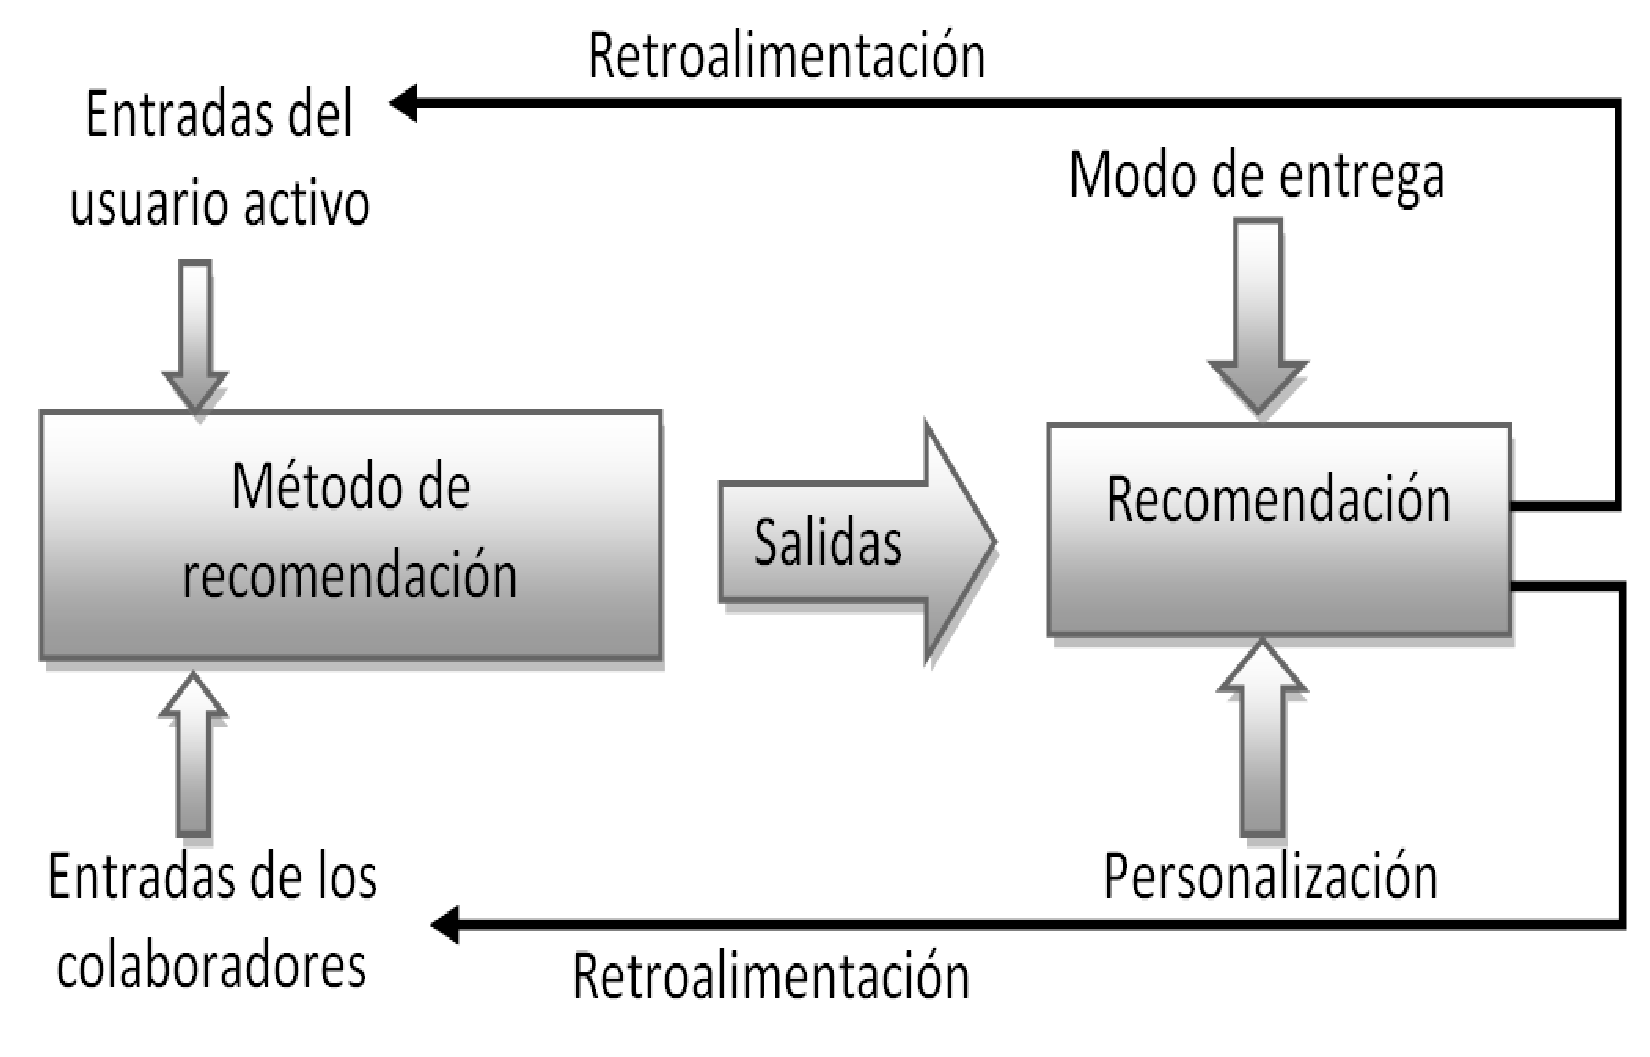
\includegraphics[width=0.6\textwidth]{./images/procesoRecomendacion2.pdf} 
} \caption{Esquema de proceso de generación de una recomendación.} 
 \label{fig:procesoRecomendacion} 
\end{figure}

\paragraph{}
La información sobre los usuarios puede venir dada de dos formas que no tienen porqué ser mutuamente exclusivas \citep{Yager2003}: por \textbf{extensión} o \textbf{intencionalmente.} Por extensión se refiere a información que se tenga sobre las experiencias pasadas del usuario con respecto a los ítems encontrados. Es lo que también conocemos como \textbf{navegación implícita} pues el usuario no es consciente de estos seguimientos. Por información expresada intencionalmente se entiende alguna especificación de los ítems deseados por los usuarios. También se le llama \textbf{navegación explícita} y consiste en que el usuario expresa intencionalmente al sistema de recomendación información sobre sus preferencias.
Estas formas de obtener información ya se han mencionado en el punto 2.2 así como algunos ejemplos.
\paragraph{}
La salida del sistema está constituida por las recomendaciones generadas por el sistema, que variarán dependiendo del tipo, cantidad y formato de la información proporcionada al usuario. Algunas de las formas más comunes de representar la salida son las siguientes:

\begin{itemize}
\item Sugerencia o lista de sugerencias al usuario de una serie de ítems.
\item Presentar al usuario predicciones del grado de satisfacción que se asignará al ítem concreto. Estas estimaciones pueden ser presentadas como personalizadas al usuario o como estimaciones generales del conjunto de colaboradores.
\item Cuando la comunidad de usuarios es pequeña o se conocen bien los miembros de dicha comunidad, podría ser útil visualizar las valoraciones individuales de los miembros que permitiría al usuario activo obtener sus propias conclusiones sobre la efectividad de una recomendación.
\end{itemize}

Independientemente de estos formatos de salida, puede resultar muy interesante incluir una breve descripción o explicación sobre el ítem recomendado a modo de justificación del porqué de dicha recomendación.

\subsection{Método de generación de recomendaciones}

En esta sección se describe una serie de métodos de recomendación que se usan habitualmente en los sistemas de recomendación, pero se debe considerar que no son mutuamente exclusivos entre sí, sino complementarios, es decir, que en un mismo sistema de recomendación  se puede usar uno o varios de estos métodos. \\
Enseguida se enuncian  los tres métodos más simples:

\begin{enumerate}
\item \textbf{Recuperación pura o recomendación nula}, en la que el sistema ofrece a los usuarios una interfaz de búsqueda a través de la cual pueden realizar consultas a una base de datos de ítems. Se trata, pues, de un sistema de búsqueda por lo que técnicamente no es un método de recomendación, aunque ante los usuarios aparece como tal.
\item Otros sistemas usan \textbf{recomendaciones seleccionadas manualmente por expertos}, como por ejemplo editores, artistas o críticos en el caso de recomendaciones de películas o cd's de música. Los expertos identifican ítems basándose en sus propias preferencias, intereses u objetivos y crean una lista de ítems que esté disponible para todos los usuarios del sistema. A menudo acompañan estas recomendaciones de comentarios de texto que puedan ayudar a los usuarios a evaluar y entender la recomendación.
\item En otros casos, los sistemas ofrecen \textbf{resúmenes estadísticos} calculados en función de las opiniones del conjunto de usuarios, por lo que tampoco son personalizados. Por ejemplo, se podrían tener en cuenta el porcentaje de usuarios a los que ha satisfecho o han comprado un artículo, número de usuarios que recomiendan un ítem, o una evaluación media de todos los usuarios con respecto al ítem.
\end{enumerate}

Estos métodos de generación de recomendaciones, por su simplicidad no son considerados propiamente métodos de generar recomendaciones en la literatura. Para generar las recomendaciones hay dos posibilidades comúnmente aceptadas que dan lugar a dos grandes grupos de sistemas de recomendación \citep{Yager2003, Porcel2004}: los sistemas de recomendación colaborativos y los no colaborativos o basados en contenidos (también conocidos como reclusivos).

\subsection{Grado de personalización}
Según su grado de personalización, también podremos clasificar los sistemas de recomendación:
\begin{itemize}
\item Cuando los sistemas de recomendación proporcionan las mismas recomendaciones a todos los usuarios, son clasificados en este ámbito como \textbf{no personalizados.} Dichas recomendaciones estarán basadas en selecciones manuales, resúmenes estadísticos u otras técnicas similares.
\item Los sistemas de recomendación que tienen en cuenta la información actual del usuario objeto de las recomendaciones, proporcionan \textbf{personalización efímera}, puesto que las recomendaciones son respuesta al comportamiento y acciones del usuario en su sesión actual de navegación.
\item Los sistemas de recomendación que ofrecen el mayor grado de personalización son los que usan \textbf{personalización persistente} ofreciendo recomendaciones distintas para distintos usuarios, incluso cuando estén buscando el mismo ítem. Estos sistemas están basados en el perfil de los usuarios, por lo que hacen uso de métodos de filtrado colaborativo, filtrado basado en contenidos o correlaciones entre ítems.
\end{itemize}

\section{Algoritmos de recomendación}
El objetivo es sugerir nuevos elementos a un usuario basándose en sus elecciones anteriores y en elecciones de gente con similar historial de valoraciones. Las formas de recoger estas valoraciones es \textbf{explícita} o \textbf{implícita.} Por ejemplo el tiempo que pasa leyendo una determinada pagina web, los enlaces que sigue, el número de veces que se escucha una canción, esta sería una aproximación más clásica de minería de datos. Una vez que se tiene suficiente información del usuario se pasa a la fase de predicción y recomendación. \\
La predicción hace referencia a estimar qué valoración daría el usuario a cada elemento mientras que recomendación se refiere a extraer los \textbf{N} elementos más recomendables (Top-N) \citep{GalanNieto1994}.

\subsection{Filtrado colaborativo basado en memoria}

Los sistemas de recomendación colaborativos recogen valoraciones expresadas como votaciones, sobre una serie de ítems en un dominio dado y tratan de emparejar personas que comparten las mismas necesidades o gustos \citep{Adomavicius2005, Herlocker1991, Ramezani0000}. Utilizan toda la base de datos de elementos y usuarios (valoraciones y opiniones) para generar predicciones y obtener recomendaciones personalizadas.\\
Este algoritmo emplea \textbf{técnicas estadísticas} para encontrar a vecinos, es decir usuarios con un historial de valoraciones sobre los elementos similar al usuario actual.  

\subsubsection*{Coeficiente de Correlación de Pearson}

Se deriva de las fórmulas de regresión lineal, y asume que la relación entre elementos es lineal, los errores independientes y la distribución tiene varianza constante y media 0. Estas suposiciones normalmente no se producen realmente con lo que hay que valorar cómo afectan a la bondad de los resultados, pero en un gran número de casos el el rendimiento utilizando \textbf{correlación de Pearson} es apropiado. El peso que se asigna al usuario \textit{u} para predecir al usuario activo a viene dado por (\textit{$r_{a,i}$} es la votación del usuario \textit{a} al elemento \textit{i}):

\begin{equation}
\displaystyle w_{a,u} = {\sum_{i=1}^{m}( r_{a,i} - \bar{r_a} )(r_{u,i}- \bar{r_u}) \over \sigma_a \sigma_u }
\end{equation}
\paragraph{}
Otras formas son las basadas en vectores (similaridad de coseno), las medidas de correlación basadas en entropía (correlación de Ringo o correlación de Spearman.)\\
Una vez se tienen los pesos de correlación de cada algoritmo hay que saber como de confiables son estos pesos. Es posible tener un alto grado de correlación con vecinos con los que se comparten pocos elementos valorados por el usuario actual, pero con igual valoración. 
\paragraph{}
El uso de estos pesos proporciona una estimaciones malas puesto que para tener una idea real de la correlación, entre más votos compartidos mejor. En los casos de pocas muestras es recomendable disminuir el factor de correlación en función del numero de votos compartidos. Para intentar mejorar más los pesos de la correlación entre usuarios se puede entrar a trabajar con la varianza de los elementos que cada usuario ha votado. \\
Si un elemento es votado positivamente por un gran porcentaje de la población, el que dos usuarios compartan esa votación dice poca información acerca de la correlación entre usuarios. Lo contrario pasa en el caso de elementos que sean votados positiva o negativamente por pocos usuarios. \\
Para tomar en cuenta este hecho se añade a la fórmula de la \textbf{correlación de Pearson} un término con la varianza del elemento.

\subsubsection*{Selección de Vecinos}

En sistemas con pocos usuarios podría ser factible trabajar con todos los usuarios como vecinos tan sólo multiplicando cada uno por el peso de su correlación. Sin embargo en los sistemas actuales que poseen miles de usuarios esta vía no es posible, por ello hay que tomar un subconjunto de los usuarios, lo que no sólo mejora la eficiencia sino también la efectividad. Para elegir el número de vecinos se puede:
\begin{enumerate}
\item Establecer un \textbf{umbral de correlación} y tomar todos los que superen dicho umbral. El problema es que puede haber usuarios que no tengan muchos vecinos con correlación alta. Por tanto el número de vecinos sería bajo y esto provocará que el número de elementos sobre el que la vecindad de un usuario puede opinar es también bajo.
\item Tomar \textbf{N vecinos} siempre, teniendo en cuenta que un número demasiado alto puede diluir la influencia de los vecinos con más peso y un número demasiado bajo provoca los mismos problemas que el método anterior.
\end{enumerate}

\subsubsection*{Recomendación}

La forma básica consiste en tomar las notas dadas por cada vecino y proporcionarlas a su correlación con el usuario actual:

\begin{equation}
\displaystyle p_{a,i} = r_a + { \sum_{u=1}^{n}(r_{u,i}-\bar{r_u}) w_{a,u} \over  \sum_{u=1}^{n} w_{a,u}}
\end{equation}

\paragraph{}
Una vez que se ha construido una \textbf{lista de vecinos} se combinan sus preferencias para generar una lista con los \textbf{N} elementos más recomendables para el usuario actual. Entre sus inconvenientes se encuentra la necesidad de disponer de un número mínimo de usuarios con un número mínimo de predicciones cada uno, incluído el usuario para el que se pretende realizar la recomendación.

\subsection{Filtrado colaborativo basado en modelo}

Desarrollan primero un modelo de las valoraciones del usuario. Tratan el problema como un problema de predicción estadística y calculan el valor esperado para cada ítem en función de las valoraciones anteriores. Para ello se utilizan distintos algoritmos de aprendizaje clustering o redes neuronales como las \textbf{Redes de Funciones de Base Radial} (RBFN).
Por ejemplo utilizando clustering se trata de clasificar un usuario en particular dentro de una clase de usuarios y a partir de ahí se estiman las probabilidades condicionadas de esa clase hacia los elementos a evaluar.\\
En general, ante las consultas responden más rápido que los basados en memoria, pero por contra necesitan de un proceso de aprendizaje intensivo. 
\paragraph{}
El consumo de memoria y de CPU de cualquier sistema de filtrado e información es muy elevado al tratar con muchos datos. La optimización de los algoritmos para mejorar su rendimiento es uno de los principales campos de investigación dentro del filtrado colaborativo.
\paragraph{}
Algunas características deseables en estos sistemas suponen una modificación constante de los datos, lo que hace necesarios algoritmos que tengan una coste de actualización bajo.
Por ejemplo los nuevos elementos han de aparecer en el sistema lo antes posible. También se requiere una mejora continua del perfil del usuario. Es decir que el usuario perciba que el \textit{esfuerzo} de evaluar nuevos elementos se vea compensado con unas mejoras en las recomendaciones que se obtienen. 
\paragraph{}
Además de los aspectos técnicos la implantación de sistemas de recomendación puede plantear problemas sociales como la privacidad de los usuarios. Es un asunto delicado ya que para tener un buen funcionamiento es necesario conocer la máxima información posible del usuario.
\paragraph{}
Una primera solución es mantener tan solo la información relacionada con las votaciones y conocer del usuario solo un seudónimo, pero esto choca con el modelo de negocio basado en publicidad que se utiliza abundantemente en la actualidad \citep{GalanNieto1994}.

\subsection{Algoritmo basado en contenido}

En este caso, en lugar de buscar similitudes entre usuarios se buscan cercanías entre ítems. El procedimiento consiste en seleccionar los elementos  que un usuario determinado ha votado y después comprobar que tan similar es cada uno  del resto de los ítems en el sistema para terminar recomendando los más parecidos \citep{Ramezani0000}. 
\paragraph{}
Existen distintas formas de evaluar la similitud entre elementos pero el procedimiento genérico consiste en tomar dos elementos \textbf{x1, x2} y después calcular su similitud a partir de todos los usuarios que han votado ambos elementos. En teoría es la misma aproximación que la que se tenía con algoritmos basados en vecinos cercanos. La ventaja es que en el caso de los elementos la similitud entre ellos es menos variable que la similitud entre usuarios, lo que permite hacer el proceso mucho más rápido \citep{Sarwar2001, Deshpande2004}.

\paragraph{}
En un sistema basado en contenido, los objetos de interés se definen por sus características asociadas. Por ejemplo, los sistemas de texto de la recomendación como el sistema de filtrado de grupo de noticias \textbf{NewsWeeder} utiliza las palabras de sus textos como rasgos. Una recomendación basada en contenido construye de un perfil de intereses de usuarios en base a las características presentes en los objetos que el usuario ha calificado. Schafer, Konstan y Riedl llaman a esto \textbf{correlación ítem-a-ítem}. \\
Al igual que en el caso del algoritmo colaborativo, el perfil de usuario en un algoritmo basado en contenido es el modelo a largo plazo y se actualiza en la medida que se tenga más información sobre las preferencias del usuario.
\paragraph{}
El funcionamiento de estos sistemas dependerá en gran medida del tipo de información de descripción que se utilice en la construcción del perfil de usuario. Esta información se puede dividir en:
\begin{description}
\item [Conjunto de características:] asociado a cada producto puede aparecer un conjunto de características que lo describe, como por ejemplo el autor de un libro, serie a la que pertenece, actores de una película, consumo medio si estamos hablando de vehículos. 
\item [Información textual sobre el producto:] es un documento que describe dicho producto (un resumen de un libro, el argumento de una película, etcétera.). La principal diferencia con respecto al conjunto de características, es que la información no está estructurada.
\end{description}

\paragraph{}
Existen sistemas basados en contenido que solo trabajan con los conjuntos de características asociados a cada ítem.  Estos tienen un esquema de  funcionamiento similar al que podemos ver en la figura \ref{fig:esquemaFC} \citep{PerezCordon2008}, se analizan las características de los productos comprados o valorados positivamente por el usuario, construyen un perfil de usuario y por último, usan este perfil de usuario para buscar nuevos productos que puedan satisfacer al usuario y los recomienda.\\

\begin{figure}[H]
 \centering 
\framebox{
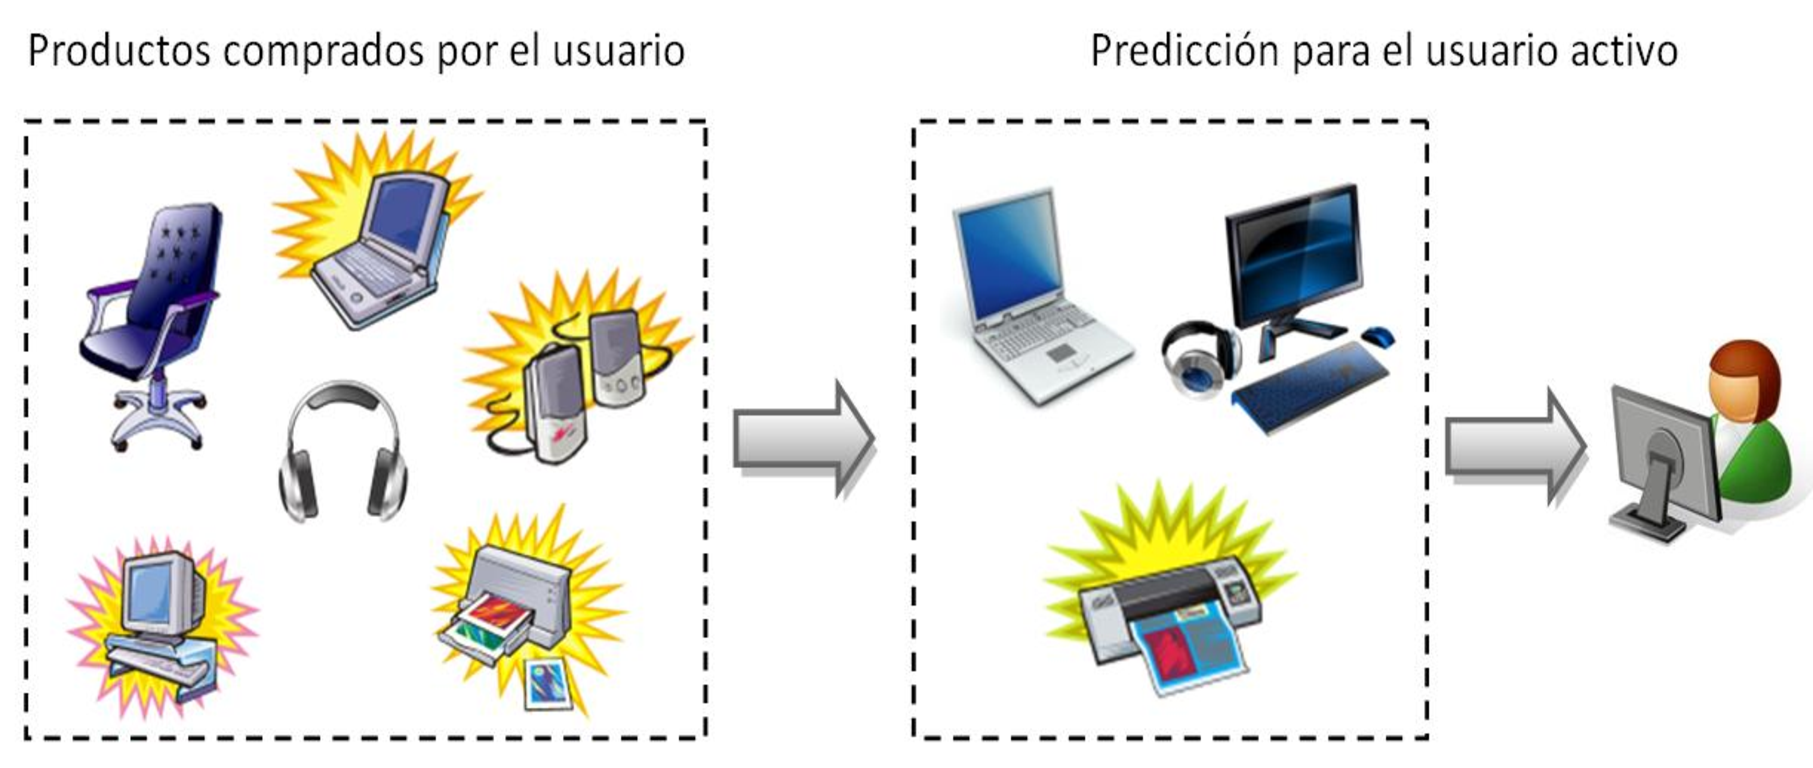
\includegraphics[width=0.9\textwidth]{./images/esquemaBC2.pdf} 
} \caption{Esquema de funcionamiento algoritmo basado en contenido.} 
 \label{fig:esquemaFC} 
\end{figure}

\subsubsection{Similaridad Basada en Coseno}

Se considera cada elemento como un vector dentro de un espacio vectorial de \textbf{M} dimensiones y se calcula la similitud como el coseno del ángulo que forman. Es decir, si tenemos dos vectores \textbf{$x_1$, $x_2$} que consisten en un array cuyos elementos son las votaciones recibidas de cada usuario. Su similitud será:

\begin{equation}
%\displaystyle Cos(x_1,x_2)={\vec{x_1} \cdot  \vec{x_2} \over \parallel \vec{x_2} \parallel \Delta \parallel \vec{x_1} \parallel} 
\displaystyle Cos(x_1,x_2)={\vec{x_1} \cdot  \vec{x_2} \over \parallel \vec{x_2} \parallel  \parallel \vec{x_1} \parallel} 
\end{equation}

\subsubsection{Cálculo de la predicción}

Una vez que se elige un método para computar la relación entre elementos quedan por calcular los elementos que son más parecidos a los del usuario. De nuevo existen varias aproximaciones.

\begin{description}
\item [Suma ponderada.] Se toman todos los elementos que el usuario ha votado. Se toma un elemento \textbf{x1} y para ese elemento se suman todos los coeficientes de similitud entre ese elemento y los elementos votados por el usuario, proporcionados al valor del voto. Siendo \textbf{N} cada elemento votado por el usuario \textbf{$S_{i,N}$} La similitud entre los elementos \textbf{i} y \textbf{N} y \textbf{$R_{u,N}$} la valoración del usuario del elemento \textbf{N}:
\begin{equation}
\displaystyle P_{u,i}={ \sum_N (S_{i,N})(R_{u,N}) \over \sum_N (S_{i,N})} 
\end{equation}
\item [Regresión.] Similar al modelo anterior, pero en lugar de sumar directamente las notas de los elementos similares se utiliza una aproximación basada en la recta de regresión. Con este método se intenta compensar un problema que se da al evaluar las similitudes mediante medidas del coseno o la correlación, y es que vectores con alta similitud pueden encontrarse distantes en sentido euclídeo. Se utiliza la misma fórmula que en el caso de la suma proporcionada pero sustituyendo:
\begin{equation}
\displaystyle  R_{u,N} \mbox{ por la ecuación }  \alpha \bar{R} i + \beta + \epsilon
\end{equation}
\end{description}

\section{Ejemplos}
Algunos ejemplos de sistemas de recomendación que actualmente funcionan en Internet y se mencionan en \citep{PerezCordon2008}, son los siguientes:
\begin{description}

\item[Fab.] El sistema de recomendación  Fab \citep{Balabanovic1997}, plantea que si únicamente recomienda a un usuario ítems similares a los que el mismo usuario ha preferido en el pasado, va limitándose a una sobre-especialización. Por otro lado,  si únicamente identifica usuarios cuyas preferencias son similares a los del usuario activo y recomienda los ítems que ellos han preferido, tiene el problema de que cuando aparecen nuevos ítems, no hay como recomendarlos hasta que alguien los use o se especifiquen  otros ítems similares; además, si hay usuarios con preferencias singulares no tendrán recomendaciones útiles. Entonces, Fab combina estas dos formas de recomendación, para lo cual, mantiene un perfil del usuario basado en el análisis del contenido, o sea de los ítems, y compara el perfil para determinar usuarios similares.

\item[Referral Web.] Es un sistema interactivo para reconstruir, visualizar y buscar redes sociales en la web. Kautz observa que, como resultado de las actividades humanas, se forman redes alrededor de temas de trabajo pero también se forman redes sociales. Referral Web asocia temas con personas expertas en tales temas, entonces, buscar información se convierte en buscar, en la red social, un experto en el área, y la cadena de referencias personales, desde el buscador hasta el experto. Los sistemas de recomendación  proporcionan recomendaciones anónimas, en cambio Referral Web proporciona referencias mediante una cadena de individuos con nombre propio.

\item [PHOAKS.]  People Helping One Another Know Stuff es un sistema de recomendación que reconoce y redistribuye recomendaciones de recursos de Web buscando en mensajes electrónicos \citep{Terveen1997}. Este sistema está basado en filtrado colaborativo, lo que hace posible que un grupo de personas hagan y reciban recomendaciones entre sí. Se distingue de otros sistemas por dos características principales: el rol de especialización y reuso. PHOAKS recomienda páginas de Web, búsca en los mensajes las opiniones que los participantes dejen acerca de estas páginas, y las selecciona si pasan ciertos requerimientos. La arquitectura de PHOAKS consiste en tres procesos principales: buscar mensajes con un patrón específico, clasificación de las instancias de los patrones y disposición de la información encontrada.

\item [Siteseer.] Es un sistema que utiliza los registros de páginas favoritas (bookmarks) de un usuario y la organización de éstos registros para la recomendación de páginas de Web relevantes \citep{Rucker1997}, puesto que los registros representan interés en el contenido y su organización indica relevancia entre los elementos. Siteseer utiliza en método de filtrado colaborativo y recomienda al usuario las páginas de electrónicas de sus \textit{vecinos cercanos}.  

\item[Amazon.] Es una compañía de comercio electrónico con sede en Seattle, estado de Washington, y fue una de las primeras grandes compañías en vender bienes a través de Internet. En la actualidad vende una gran variedad de productos, desde libros hasta ropa, pasando por artículos electrónicos, cds de música, software, muebles, comida, etc. Amazon se ha establecido en varios países como Canada, Reino Unido, Alemania, Austria, Francia, China y Japón para poder ofrecer los productos en estos países.  Amazon fue fundada como cadabra.com por Jeff Bezos en 1994 y lanzada en 1995. Cadabra.com comenzó como una librería en línea que tenía mas de 200.000 títulos que se podían comprar por correo electrónico. Tiempo después, su nombre fue cambiado a Amazon, por el río sudamericano del mismo nombre. Amazon implementa una gran variedad de sistemas de recomendación, tanto clásicos, como híbridos. Por ejemplo, parte de las recomendaciones que generan parecen estar hechas por un sistema de recomendación basado en contenido, que utiliza las descripciones de los productos valorados positivamente por el usuario para encontrar otros nuevos. Para valorar estos productos usa una escala de 1 al 5 de estrellas donde el uno es la valoración más baja y significa que no le ha gustado y el 5 la más alta.

\item[Zagat.] Es una empresa americana fundada en 1979 por Tim y Nina Zagat que se dedica a la edición de todo tipo de guías de restaurantes, hoteles, clubes o tiendas de distintas ciudades de los Estados Unidos y Canadá \citep{Resnick1997}. En \textit{www.zagat.com} los usuarios registrados pueden votar distintos aspectos del local preferido y, además, introducir pequeños comentarios con su experiencia. En base a estas votaciones los responsables de la empresa asignan su puntuación en sus guías anuales y hacen recomendaciones individuales a sus usuarios a través de su web. Estas recomendaciones son hechas por un sistema de recomendación  colaborativo. Zagat es la página Web comercial que utiliza un sistema de recomendación colaborativo, donde las valoraciones de los restaurantes son actualizadas constantemente por los usuarios. Incluye muchas opciones de búsquedas avanzadas donde el usuario puede especificar sus criterios de búsqueda en categorías tales como comida, decoración, costos, etcétera, o restringir la búsqueda a cierta área o un tipo de cocina concreta.
\end{description}

Enseguida se muestra un cuadro comparativo \citep{Resnick1997} de los sistemas de recomendación mencionados.

\begin{table}[H]
\begin{small}
\caption{Cuadro comparativo de sistemas de recomendación.} \begin{center}
\linespread{0.9}\selectfont
\begin{tabular}{>{\footnotesize}p{0.8in}>{\footnotesize}p{0.8in}>{\footnotesize}p{0.8in}>{\footnotesize}p{0.8in}>{\footnotesize}p{0.8in}>{\footnotesize}p{0.8in}}
\hline                  
         & El contenido de la recomendación & ¿La entrada es explícita? &  ¿Es anónimo? & Modo de agregación  & Uso de las recomendaciones \\
\hline             
Fab  & Numérica: 1-7. & Explícita. & Pseudónimo. & Ponderación personalizada; combinada con análisis de contenido.  & Selección/filtrado. \\

ReferralWeb & Mención de una persona o un documento. & Extraídas de fuentes públicas de datos. & Atribuído.  & Montar cadena de referencias a la persona deseada.  & Pantalla. \\

PHOAKS & Mención de una URL. & Extraídos de publicaciones Usenet.  & Atribuído.  & Una persona, un voto (por URL). & Ordenados en pantalla. \\

Siteseer  & Mención de una URL. & Extraídos de las carpetas de marcadores existentes. & Anónimo. & Frecuencia de mención en la superposición de las carpetas. & Pantalla.\\

Amazon & Numérica:1-5. & Explícita. & Pseudónimo.  & Por cliente, valora todos los productos comprados. &  Pantalla.  \\

Zagat  & Numérica: 0-3. & Explícita. & Pseudónimo. & Por usuario, valora todos los aspectos de un establecimiento. & Pantalla, sugerencias de los demás usuarios.  \\

\hline
\end{tabular}
\label{tab:cuadro}
\end{center}
\end{small}
\end{table}

\section{Lógica difusa}

La lógica difusa o lógica heurística\footnote{No necesariamente es heurística en todos los problemas donde se aplica este concepto. La lógica difusa se basa en la experiencia humana para definir un problema de forma imprecisa, pero si el problema es complejo para llegar a una solución requiere de otros métodos (usualmente matemáticos) que no se basan en heurística.} se basa en lo relativo de lo observado \citep{wikipedia2}. Este tipo de lógica toma dos valores aleatorios, pero contextualizados y referidos entre sí. Así, por ejemplo, una persona que mida 2 metros es claramente una persona alta, si previamente se ha tomado el valor de persona baja y se ha establecido en 1 metro. Ambos valores están contextualizados a personas y referidos a una medida métrica lineal.
\paragraph{}
La lógica difusa se adapta mejor al mundo real en el que vivimos e incluso puede comprender y funcionar con nuestras expresiones, del tipo \textit{hace mucho calor}, \textit{no es muy alto}, el ritmo del corazón está \textit{un poco acelerado}, etcétera. La clave de esta adaptación al lenguaje, se basa en comprender los cuantificadores de nuestro lenguaje (\textit{mucho}, \textit{muy} y  \textit{un poco}).
\paragraph{}
En la teoría de conjuntos difusos se definen también las operaciones de unión, intersección, diferencia, negación o complemento, y otras operaciones sobre conjuntos en los que se basa esta lógica.
Para cada conjunto difuso, existe asociada una función de pertenencia para sus elementos, que indican en qué medida el elemento forma parte de ese conjunto difuso. Las formas de las funciones de pertenencia más típicas son trapezoidal, lineal y curva (gaussiana).

\subsection{Sistemas de Inferencia Difuso}

El \textbf{Sistema de Inferencia Difuso} (FIS por sus siglas en inglés) es un framework de computación popular basado en los conceptos de Teoría de conjuntos difusos, reglas difusas \textbf{si-entonces} y razonamiento difuso \citep{Jang1997}.
\paragraph{}
Se han desarrollado aplicaciones exitosas en una amplia  variedad de campos, tal como el control automático, clasificación de datos, análisis de decisión, sistemas expertos, predicción de series de tiempo, robótica y patrones de reconocimiento. 
Debido a su carácter multidisciplinario, el  sistema de inferencia difuso es reconocido también como sistema basado en reglas difusas, sistema experto difuso, modelo difuso, memoria asociativa difusa, controlador lógico difuso, y simplemente (sin ambigüedades) sistema difuso.
\paragraph{}
La \textbf{estructura básica} de un sistema de inferencia difuso consiste de tres componentes conceptuales: 
\begin{enumerate}
\item Una regla base que contiene una selección de reglas difusas.
\item Una base de datos (o diccionario) que define las funciones de membresía usadas en las reglas difusas.
\item Un mecanismo de razonamiento que realiza el procedimiento de inferencia y hechos dados para obtener una salida razonable o conclusión.
\end{enumerate}
\paragraph*{}

El sistema de inferencia difuso básico puede tomar entradas difusas o entradas numéricas (vistas como singletons), pero las salidas que produce son casi siempre conjuntos difusos.\\
Algunas veces es necesario  que tenga una valor numérico, especialmente en una situación donde un sistema de inferencia difuso es usado como controlador. Por lo tanto,  necesitamos un método de defuzificacion para extraer un valor que mejor represente al conjunto difuso. 
\paragraph{}
Un sistema de inferencia difuso  con una salida de un valor numérico se muestra en la figura \ref{fig:fuzzy11} \citep{Jang1997} donde la línea discontinua indica un sistema de inferencia difuso básico con salida difusa y el bloque de defuzificación  responde al propósito de transformar un conjunto difuso de salida en un sólo valor. \\

\begin{figure}[H] 
 \centering 
\framebox{
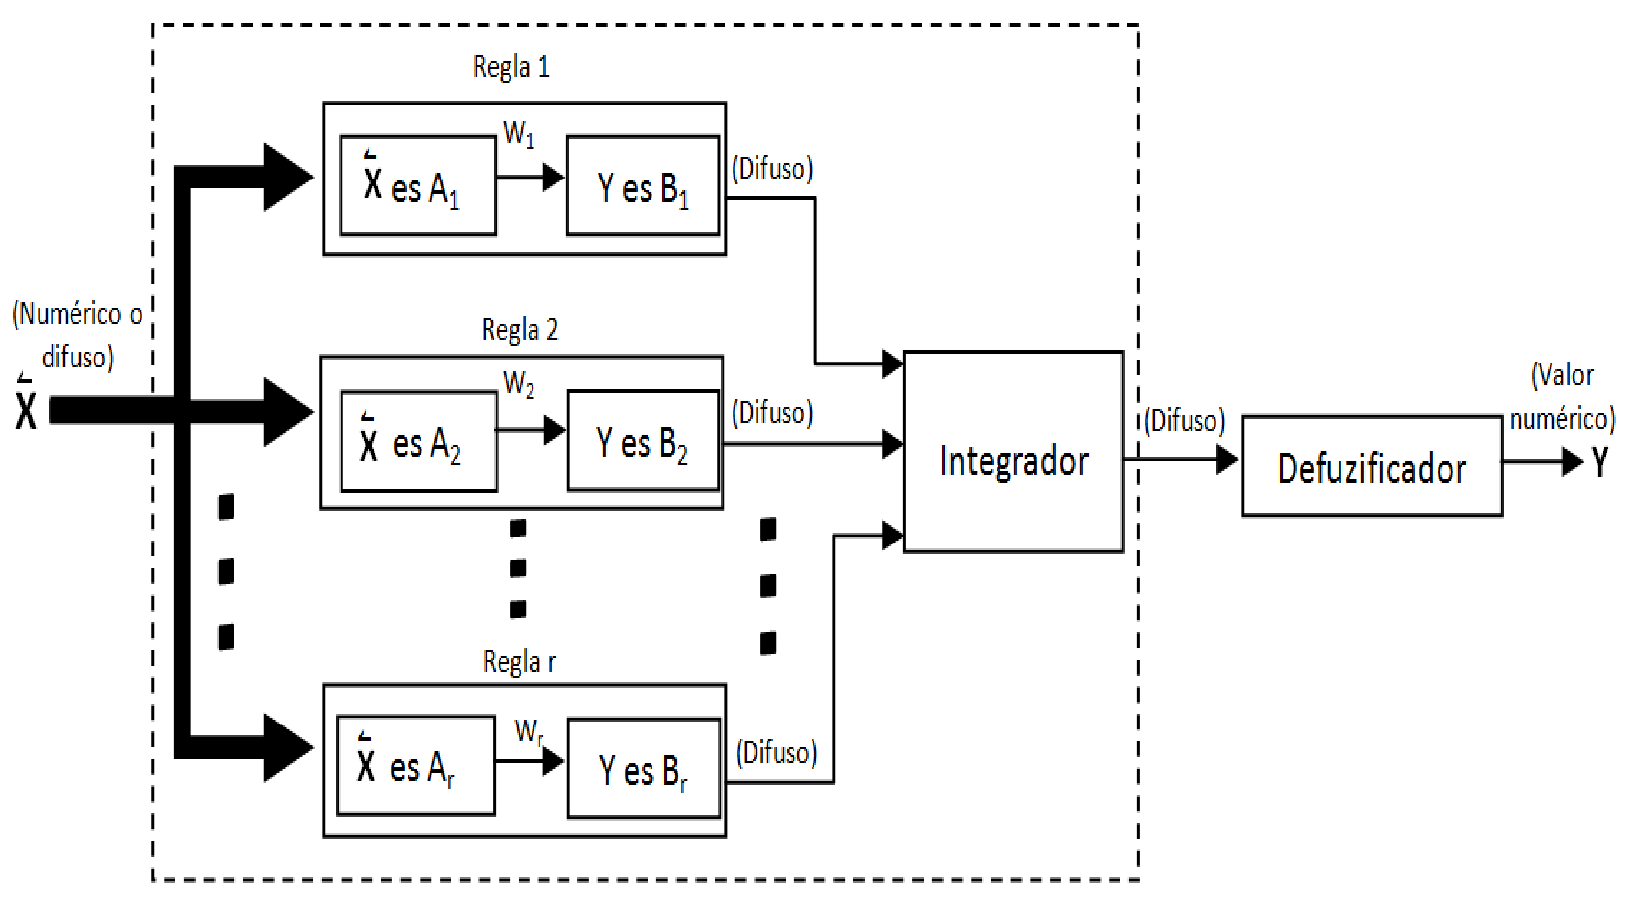
\includegraphics[width=0.6\textwidth]{./images/fuzzy11.pdf} 
} \caption{Diagrama de bloques para un Sistema de Inferencia Difuso.} 
 \label{fig:fuzzy11} 
\end{figure}

\paragraph{}
Con entradas y salidas numéricas, un sistema de inferencia difuso implementa un mapeo no lineal de su espacio de entrada a su espacio de salida. Este mapeo es realizado por un número de reglas difusas \textbf{si-entonces}, cada una de ellas describe el comportamiento local del  mapeo. En particular, el antecedente de  una regla define  una región difusa en el espacio de entrada, mientras el consecuente especifica la salida en la región difusa.

\subsubsection{Sistema difuso tipo Mamdani}

Si adoptamos máximos y productos algebraicos como de elección para los operadores \textbf{T-norm} y \textbf{T-conorm}, respectivamente, y usamos la composición \textbf{máximo-producto} en lugar  de la composición original \textbf{máximo-mínimo}, entonces el resultado del razonamiento difuso se muestra en la figura \ref{fig:fuzzy22} \citep{Jang1997}, donde la salida inferida de cada regla es un conjunto difuso  reducido por su fuerza de disparo a través del producto algebráico.  Otras variantes son posibles si se usan diferentes operadores \textbf{T-norm} y \textbf{T-conorms}. \\

\begin{figure}[H] 
 \centering 
\framebox{
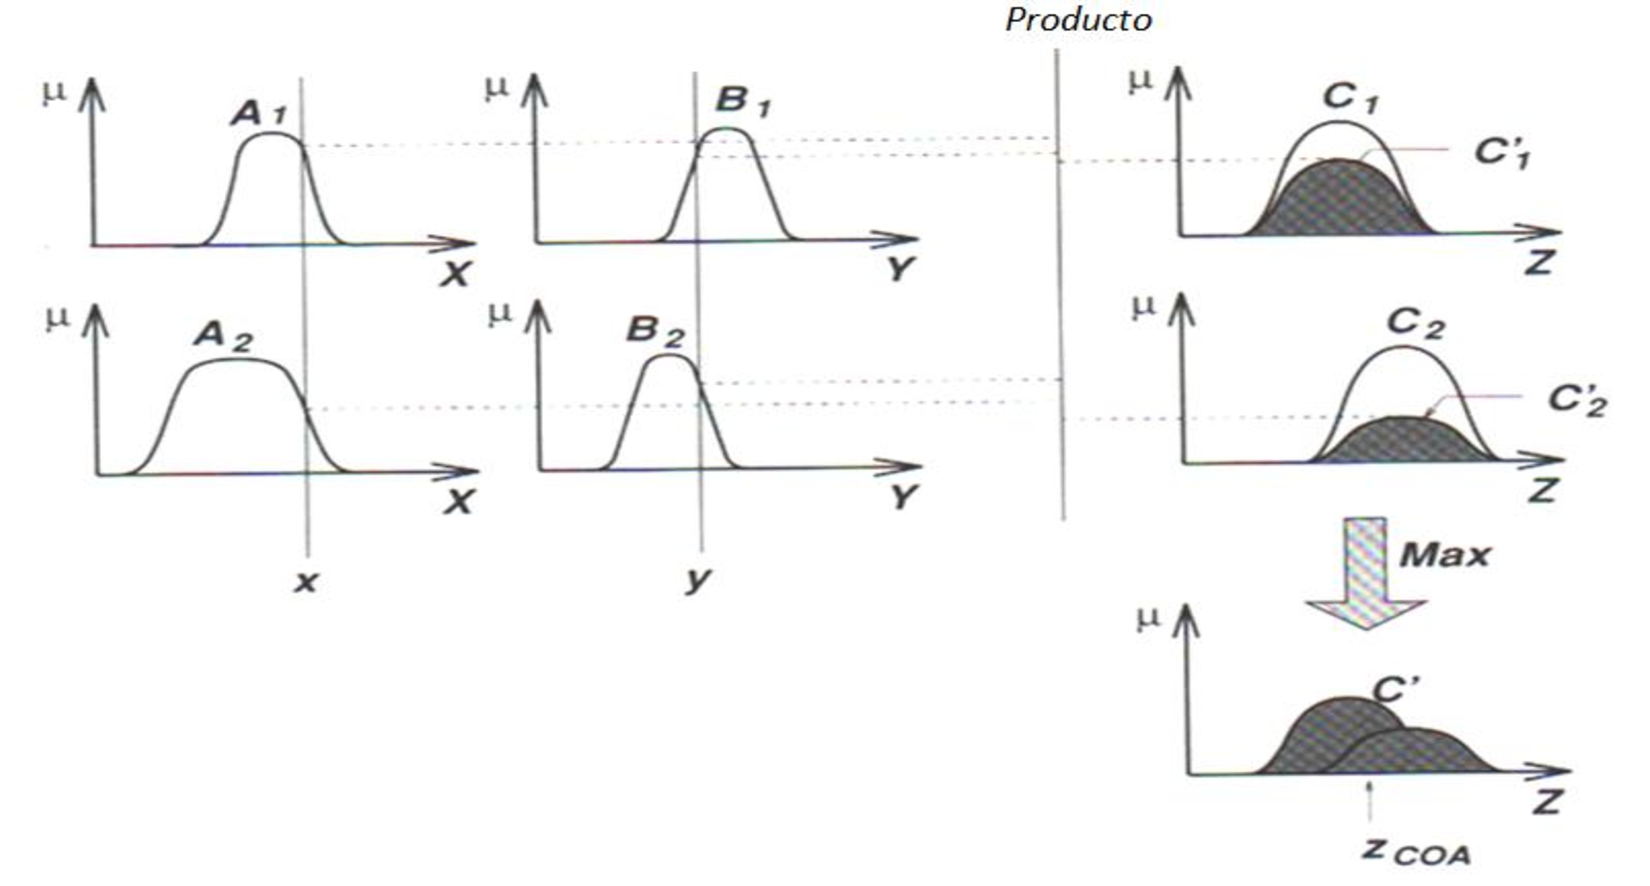
\includegraphics[width=0.6\textwidth]{./images/fuzzy22.pdf} 
} \caption{Sistema de inferencia difuso tipo Mamdani usando producto y máximo.} 
 \label{fig:fuzzy22} 
\end{figure}

\subsubsection{Sistema difuso tipo Sugeno}

El modelo difuso Sugeno fue propuesto por \textit{Takagi Sugeno y Kang} en un esfuerzo por desarrollar un enfoque sistemático para la generación de reglas difusas a partir de \textit{entradas-salidas} de un conjunto de datos. Una típica regla difusa en un modelo difuso Sugeno tiene la forma:
\begin{verbatim}
Si x  es  A  y  y  es  B  entonces  z=f(x, y),
\end{verbatim}
\paragraph{}
Donde \textbf{A} y \textbf{B} son conjuntos difusos en el antecedente,  mientras \textbf{z = f (x, y)} es una función en el consecuente como se muestra en la figura \ref{fig:fuzzy33} \citep{Jang1997}. Usualmente \textbf{f (x, y)} es un polinomio en las variables de entrada \textbf{x} y \textbf{y}, pero puede ser alguna función siempre y cuando apropiadamente pueda  describir  la salida del modelo dentro de la región difusa especificada por el antecedente de la regla. Cuando \textbf{f (x, y)} es polinomio de primer orden,  el resultado del sistema de inferencia difuso es llamado modelo difuso Sugeno de primer orden.
\paragraph{}
Cuando la función es constante tenemos un modelo difuso Sugeno de orden cero, el cual puede ser visto como un caso especial del sistema de inferencia difuso Mamdani, en el cual cada consecuente de la regla es especificado por un \textbf{singleton difuso.}\\
Las salidas de un modelo Sugeno de orden cero es una función numérica de sus variables de entrada siempre que las funciones de membresía vecinas en el antecedente tengan suficiente traslape.\\

\begin{figure}[H] 
 \centering 
\framebox{
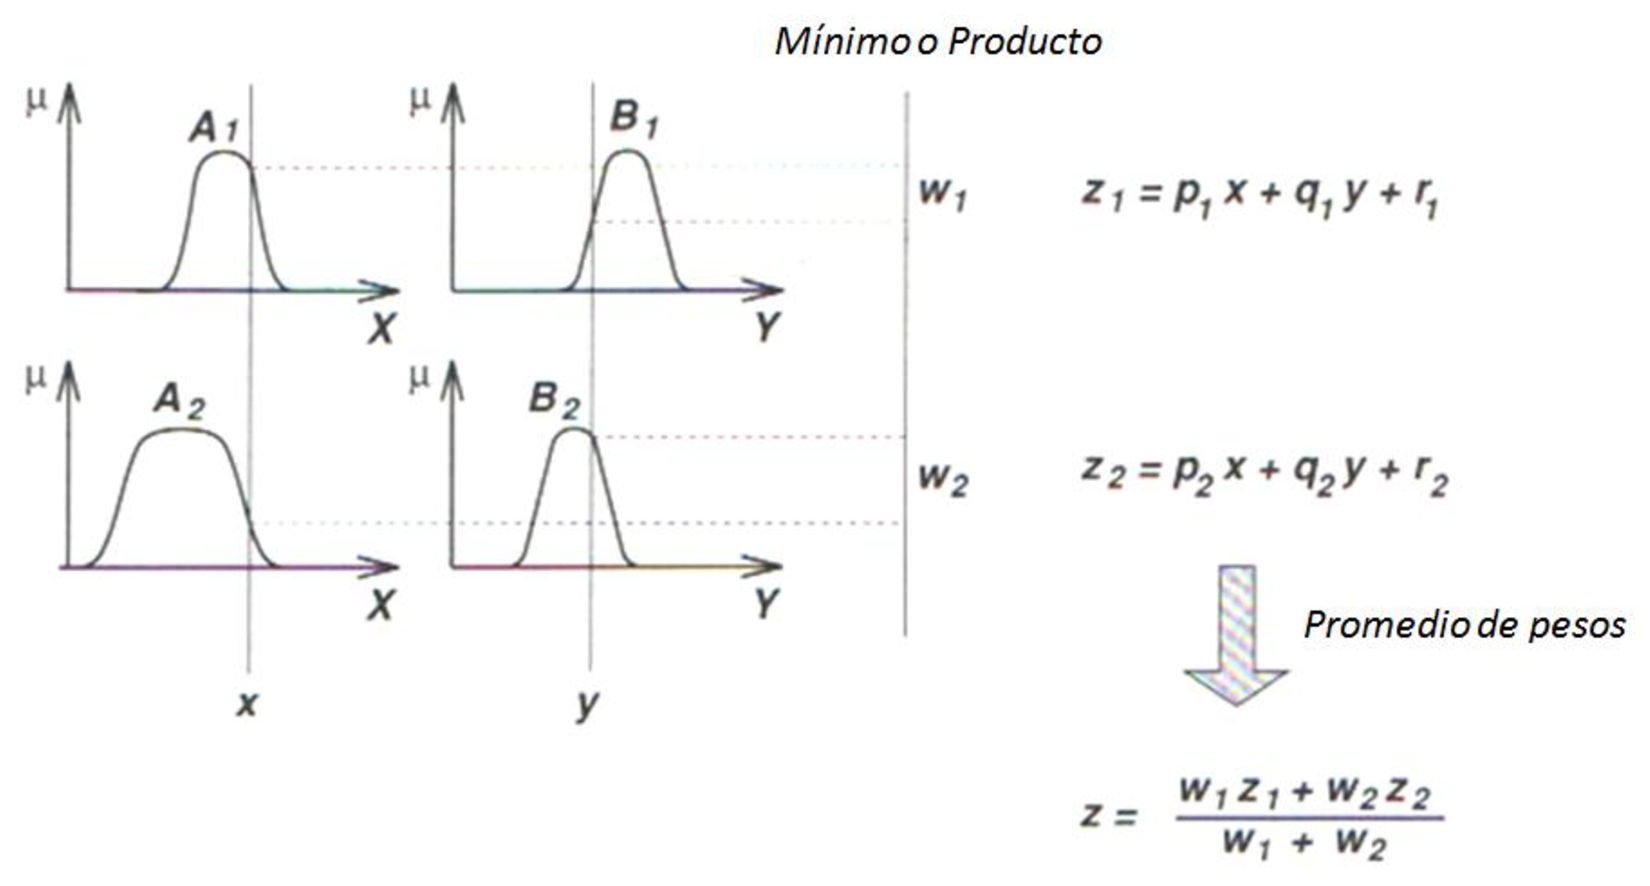
\includegraphics[width=0.6\textwidth]{./images/fuzzy33.pdf} 
} \caption{Sistema de Inferencia Difuso tipo Sugeno.} 
 \label{fig:fuzzy33} 
\end{figure}


\chapter[Arquitectura]{Arquitectura}

\section{Modelo de datos}

Cada  restaurante tiene sus propias características que lo hacen diferente a los demás, este modelo permite la manipulación de estas características. Dentro de los \textbf{atributos} encontramos ocho agrupaciones, de las cuales se derivan todos los servicios que puede tener un restaurante (salones, ambiente, calidad, etcétera). La variedad de tipos de cocina es adaptable a los usuarios ya que es bastante amplia.  
\paragraph{}
Para el usuario, permite la definición de sus gustos a través de un \textbf{perfil}, encontramos contenedores  para manipular los restaurantes que son de su agrado, que le disgustan o que le interesaría conocer.
Así también el modelo permite almacenar \textbf{reseñas} (opiniones) de restaurantes que cada usuario puede compartir con los demás usuarios registrados.
\paragraph{}
El modelo de datos representado en la figura \ref{fig:bd} \citep{Garciavaldez2009} es fácilmente adaptable a la adición de nuevos grupos de servicios y tipos de cocina para ampliar la variedad en ambos casos y ofrecer mejores recomendaciones. \\

\begin{figure}[H] 
 \centering 
\framebox{
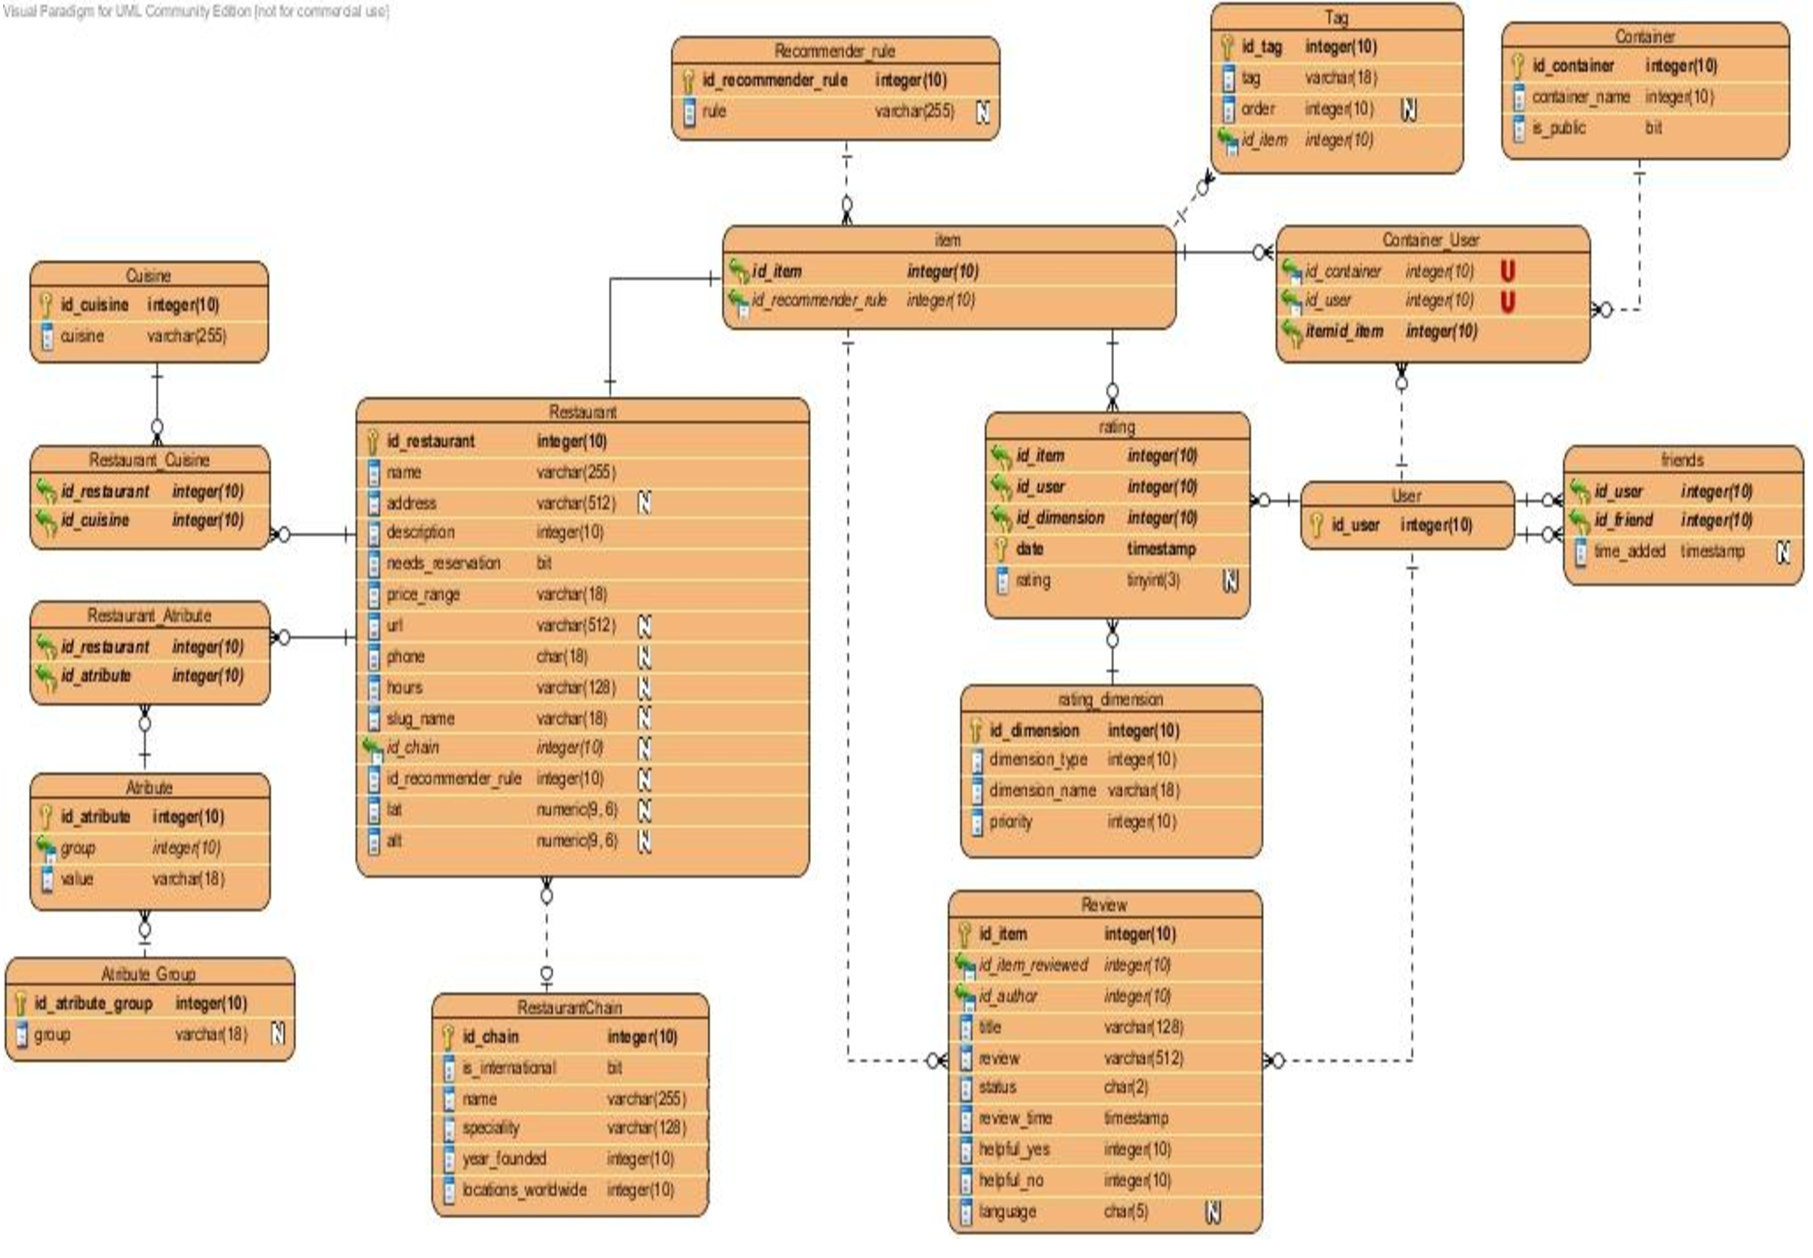
\includegraphics[width=0.9\textwidth]{./images/bd.pdf} 
}\caption{Modelo de datos del sistema.} 
 \label{fig:bd} 
\end{figure}

\section{Sistema de recomendación híbrido}

En este sistema de recomendación se ha implementado un \textbf{modelo de hibridación mediante pesos} \citep{Burke2002}, este mecanismo hace que los algoritmos de recomendación generen recomendaciones simultáneamente las cuales son  evaluadas para asignarle un peso a cada recomendación. La predicción final se calcula a partir del promedio de los pesos de las recomendaciones generadas  por los algoritmos.
\paragraph{}
Los algoritmos de recomendación utilizados son el \textbf{colaborativo} y el \textbf{basado en contenido}. El filtrado colaborativo toma la información de la \textbf{matriz de valoraciones} y en base al algoritmo de \textbf{k} vecinos más cercanos recomienda restaurantes al usuario.  El basado en contenido utiliza las \textbf{características} de los restaurantes  para buscar en la base de datos los restaurantes más parecidos a los que ha valorado positivamente el usuario activo.  A continuación se describen más detalladamente estos algoritmos.

\subsection{Módulo de filtrado colaborativo}

El filtrado colaborativo agrega valoraciones o recomendaciones de los objetos, identifica los gustos comunes de los usuarios basándose en sus valoraciones y genera una nueva recomendación tomando en cuenta las comparaciones entre los usuarios. El perfil del usuario consiste en un vector de objetos \textbf{$\displaystyle I = [ i_{1}, i_{2},...i_{n}] $} y las valoraciones de los usuarios  \textbf{$\displaystyle U = [ u_{1}, u_{2},...u_{m}]$} entonces el perfil del usuario activo lo representa como:

\begin{equation}
\displaystyle U_{j} = [u^{j}_{1}, u^{j}_{2},...u^{j}_{n}]
\end{equation}

\paragraph{}
Se utiliza el algoritmo de \textbf{K} vecinos más cercanos para identificar los usuarios con preferencias similares al usuario activo y así generar una lista de recomendaciones conocida como \textbf{Top-N}.
El sistema obtiene la similaridad entre el usuario activo y los demás usuarios utilizando la \textbf{correlación de Pearson} especificada abajo.  Esta refleja los restaurantes que son preferidos por el usuario. 

\begin{equation}
\displaystyle
P(I_{x}, I_{y}) = {\sum_{i=1}^{n}(I_{xi} - \overline{I})^2 (I_{yi}- \overline{I})^2 \over  
\sqrt{\sum_{i=1}^{n}(I_{xi}- \overline{I})^2 \sum_{i=1}^{n}(I_{yi}- \overline{I})^2}}
\end{equation}

\paragraph{}
Esquemáticamente  podemos ver el funcionamiento del filtrado colaborativo en la figura \ref{fig:filtradoColaborativo} que se muestra abajo. El algoritmo obtiene la lista \textbf{Top-N} para el usuario activo, el cual es utilizado como parámetro en el sistema de inferencia difuso que obtiene una recomendación final  mediante el promedio de pesos como en \citep{Garciavaldez2009}.

\begin{figure}[H] 
\centering 
\framebox{
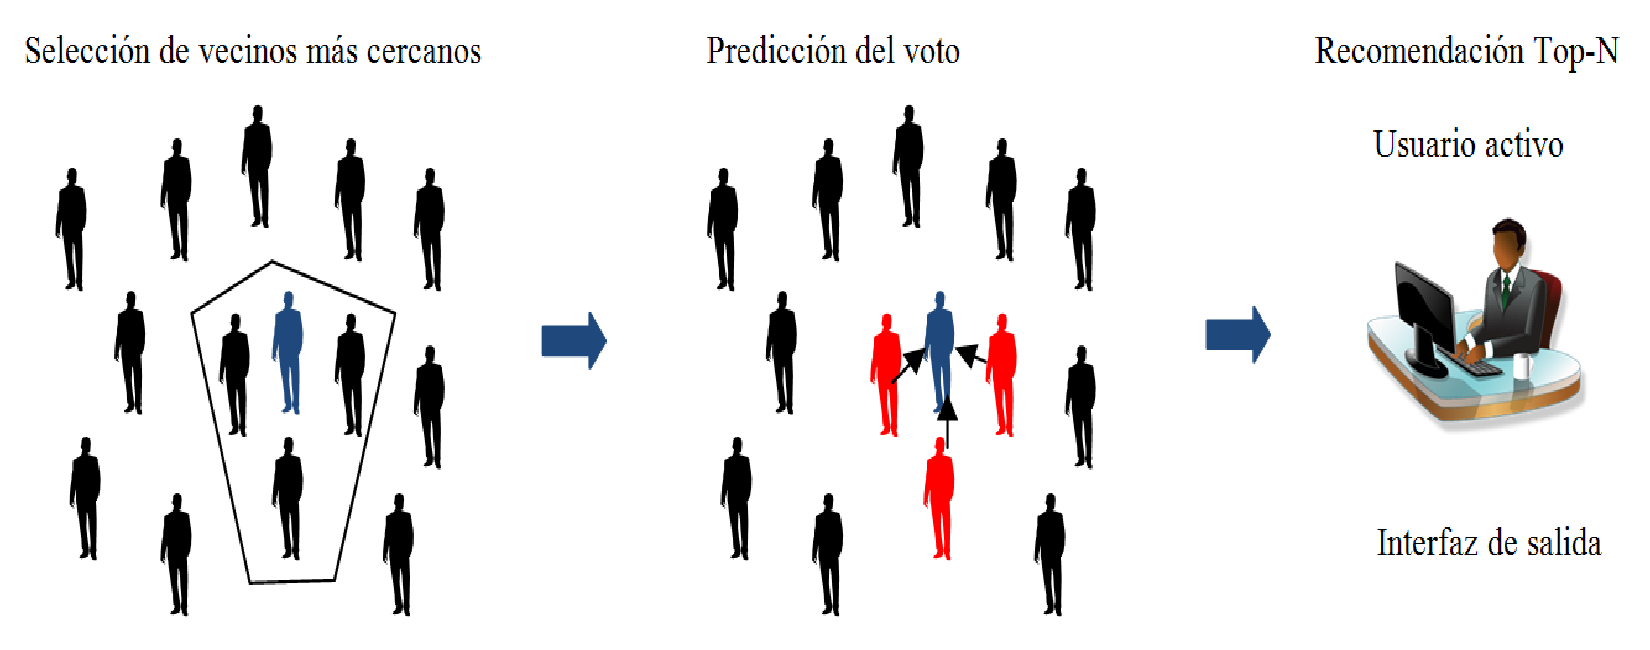
\includegraphics[width=0.6\textwidth]{./images/filtradoColaborativo.pdf} 
} \caption{Esquema de funcionamiento del algoritmo de filtrado colaborativo.} 
\label{fig:filtradoColaborativo} 
\end{figure}

\subsection{Módulo basado en contenido}

El algoritmo basado en contenido analiza las descripciones de los restaurantes que han sido valorados positivamente por el usuario. Utiliza \textbf{vectores binarios} para representar el perfil de cada restaurante. Las características que se definen en el perfil son el \textbf{rango de precios, el tipo de cocina} y los \textbf{servicios} que ofrece un  restaurante en particular. El proceso del algoritmo se muestra en la figura \ref{fig:basadoContenido} mostrada abajo.\\

\begin{figure}[H] 
\centering 
\framebox{
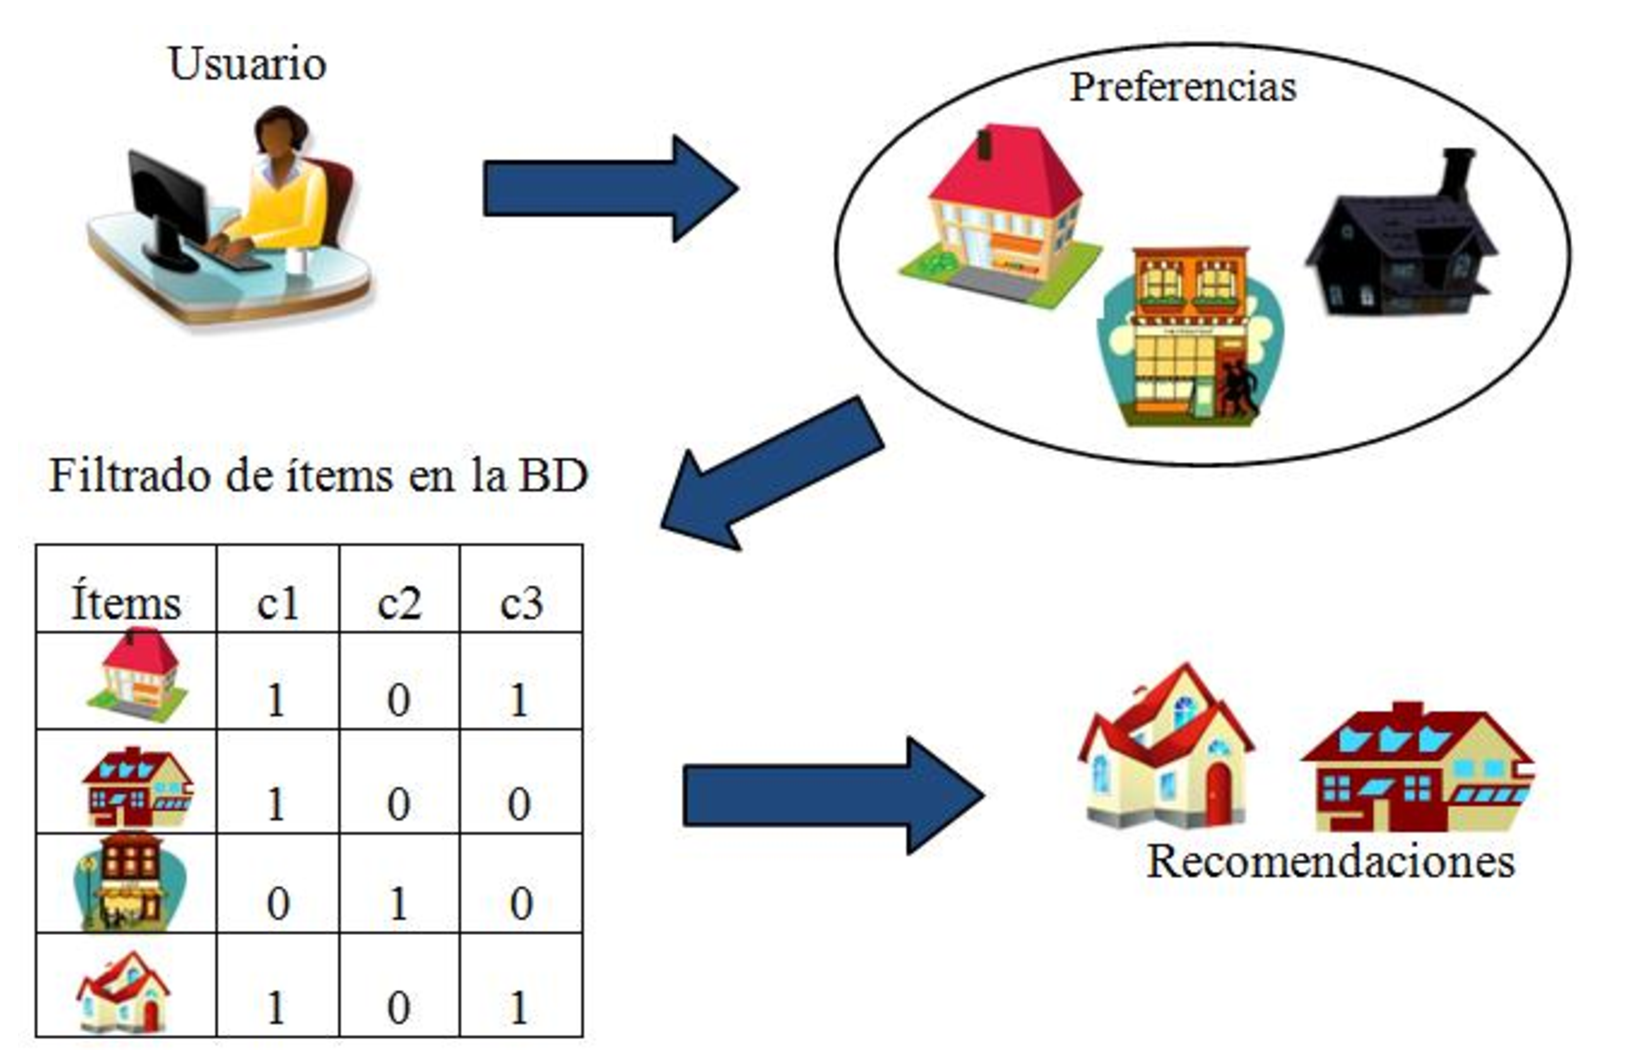
\includegraphics[width=0.6\textwidth]{./images/basadoContenido.pdf} 
} \caption{Esquema de funcionamiento del algoritmo basado en contenido.} 
\label{fig:basadoContenido} 
\end{figure}

\paragraph{}
El proceso es repetitivo para cada una de las preferencias del usuario, es decir, los restaurantes que el usuario activo ha votado con una valoración alta, y así hasta obtener la lista de recomendaciones \textbf{(Top-N)}, también será utilizada como un parámetro dentro del sistema de inferencia difuso para la recomendación final. La distancia entre los restaurantes es calculada con la \textbf{similaridad de cosenos}:

\begin{equation}
\displaystyle
 S(I_{x},I_{y})= Cos (\vec{I_{x}}, \vec{I_{y}}) ={\vec{I_{x}} \cdot  \vec{I_{y}} \over \parallel \vec{I_{x}} \parallel_{2} \cdot \parallel \vec{I_{y}} \parallel_{2}} = {\sum_{i=1}^{n} I_{i,x} I_{i,y} \over \sqrt{\sum_{i=1}^{n} I_{i,x}^{2}} \sqrt{\sum_{i=1}^{n} I_{i,y}^{2}}} 
\end{equation}
\paragraph{}
Esta fórmula obtiene la correlación entre vectores de perfil y permite identificar cuáles son los restaurantes más parecidos que serán listados para la recomendación.

\section{Sistema difuso para la selección de recomendación}

En la arquitectura se define un \textbf{sistema difuso experto} en el sistema de recomendación (módulo de recomendaciones de inferencia difuso) se muestra en la figura \ref{fig:fisExperto}. \\

\begin{figure}[H] 
\centering 
\framebox{
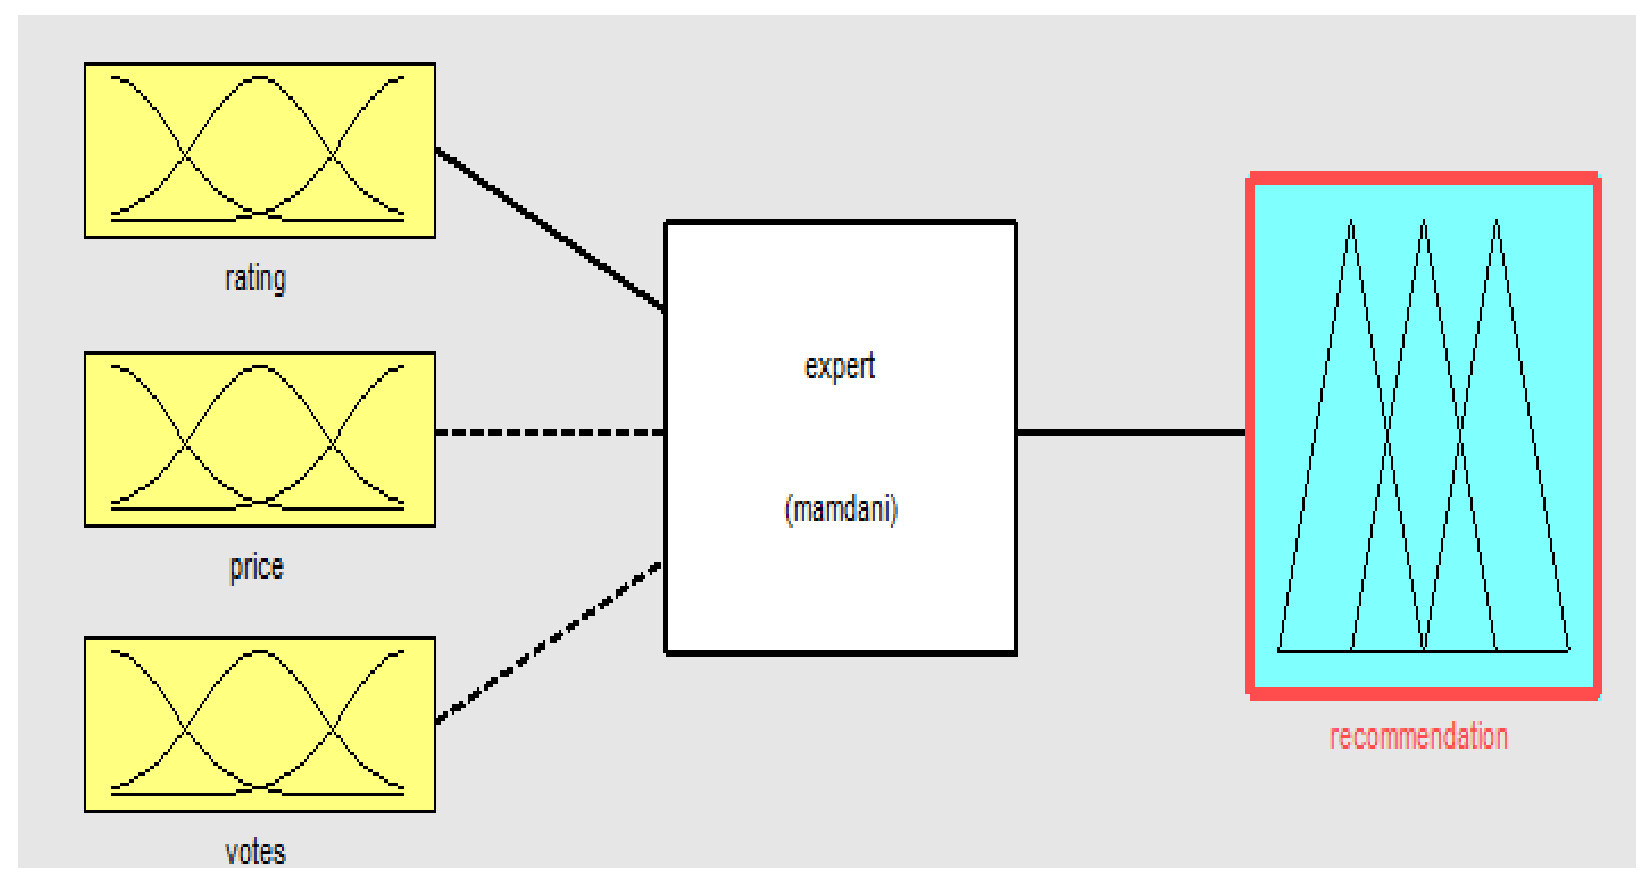
\includegraphics[width=0.7\textwidth]{./images/fisExperto.pdf} 
} \caption{Sistema de inferencia difuso del experto.} 
\label{fig:fisExperto} 
\end{figure}

\paragraph{}
Este sistema difuso basa sus recomendaciones en tres parámetros de entrada que son el \textbf{promedio de valoraciones} (rating), el \textbf{rango de precios} (price) y el \textbf{total de votos} (votes) estas características son obtenidas de cada restaurante de la base de datos y el sistema las utiliza para obtener una recomendación.
Este sistema difuso funciona como un \textbf{experto en restaurantes}, identifica la calidad de la comida, el buen servicio en un restaurant, los precios adecuados y demás aspectos que son importantes para los clientes que visitan un establecimiento.
\paragraph*{}
Considerando los parámetros de entrada mencionados anteriormente, este sistema difuso se basa en  5 reglas:

\begin{enumerate}
\item \textit{if rating is high and price is low then recommendation is high.}
\item \textit{if rating is high and votes is sufficient then recommendation is high.}    
\item \textit{if rating is high and votes is insufficient then recommendation is medium.}    
\item \textit{if rating is low and price is high then recommendation is low.}   
\item \textit{if rating is low and votes is insufficient then recommendation is low.}
\end{enumerate}

Estas reglas están basadas en la experiencia de un experto en el área, en lenguaje natural expresan lo siguiente:

\begin{enumerate}
\item \textit{Si la valoración es alta y el rango de precios es bajo entonces la recomendación es alta.}
\item \textit{Si la valoración es alta y la cantidad de votos es suficiente entonces la recomendación es alta.}
\item \textit{Si la valoración es alta y el rango de precios es bajo entonces la recomendación es alta.}
\item \textit{Si la valoración es alta y el rango de precios es alto entonces la recomendación es baja.}
\item \textit{Si la valoración es baja y la cantidad de votos es insuficiente entonces la recomendación es baja.}
\end{enumerate}
\paragraph{}
Como se observa en las reglas,  el experto asigna más peso al promedio de las valoraciones de los usuarios que han votado un restaurante en particular. La recomendación del experto tendrá un alto valor solamente cuando se dispare alguna de las dos primeras reglas.
\paragraph{}
En la figura \ref{fig:fisIntegrador} se define segundo sistema de inferencia difuso que, en base a la información de usuarios y restaurantes, asignará un peso a cada recomendación generada por los algoritmos, estos pesos son necesarios para obtener un promedio y generar una recomendación.  \\

\begin{figure}[H] 
\centering 
\framebox{
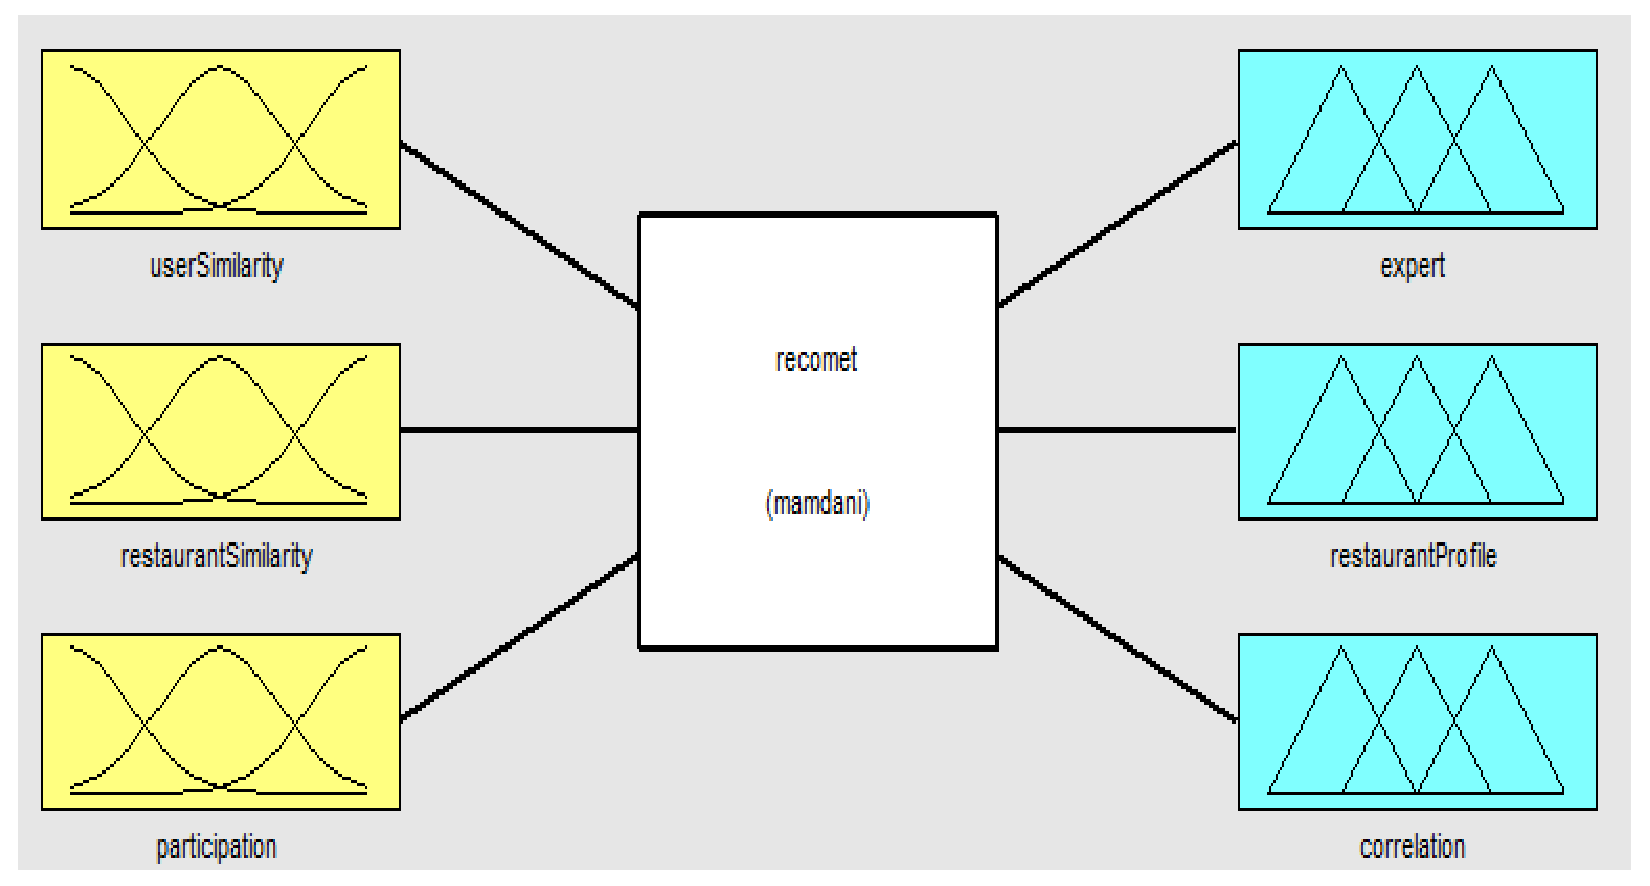
\includegraphics[width=0.7\textwidth]{./images/fisIntegrador.pdf} 
} \caption{Sistema de inferencia difuso para asignar pesos a los algoritmos.} 
\label{fig:fisIntegrador} 
\end{figure}

Este sistema difuso esta basado en 12 reglas expresadas de la siguiente manera:

\begin{enumerate}
\item \textit{if userSimilarity is low and restSimilarity is low 
 and participation is insufficient then expert is high 
 and restProfile is low and correlation is low.}
 
\item \textit{if userSimilarity is low and restSimilarity is low 
 and participation is sufficient then expert is low 
 and restProfile is low and correlation is high.}
 
\item \textit{if userSimilarity is low and restSimilarity is low 
 and participation is minimum then expert is low 
 and restProfile is low and correlation is high.}
 
\item \textit{if userSimilarity is low and restSimilarity is high 
 and participation is insufficient then expert is low 
 and restProfile is high and correlation is low.}
 
\item \textit{if userSimilarity is low and restSimilarity is high 
 and participation is minimum then expert is low
 and restProfile is high and correlation is low.}
   
\item \textit{if userSimilarity is low and restSimilarity is high
 and participation is sufficient then expert is low 
 and restProfile is high and correlation is low.}   
 
\item \textit{if userSimilarity is high and restSimilarity is low 
 and participation is insufficient then expert is low 
 and restProfile is low and correlation is high.}     
   
\item \textit{if userSimilarity is high and restSimilarity is low 
 and participation is minimum then expert is low 
 and restProfile is low and correlation is high.}  
 
\item \textit{if userSimilarity is high and restSimilarity is low 
 and participation is sufficient then expert is low 
 and restProfile is low and correlation is high.}
    
\item \textit{if userSimilarity is high and restSimilarity is high 
 and participation is insufficient then expert is low 
 and restProfile is low and correlation is high.}
 
\item \textit{if userSimilarity is high and restSimilarity is high 
 and participation is minimum then expert is low 
 and restProfile is low and correlation is high.}
 
\item \textit{if userSimilarity is high and restSimilarity is high 
 and participation is sufficient then expert is low 
 and restProfile is low and correlation is high.}

\end{enumerate}
\paragraph*{}
Estas reglas en lenguaje natural expresan lo siguiente:

\begin{enumerate}
\item \textit{Si la similaridad del usuario es baja y la similaridad de restaurantes es baja y la participación es insuficiente, entonces el experto es alto y el perfil del restaurante es bajo y la correlación es baja. }  
\item \textit{Si la similaridad del usuario es baja y la similaridad de restaurantes es baja y la participación es suficiente, entonces el experto es bajo y el perfil del restaurante es bajo y la correlación es alta.}   
\item \textit{Si la similaridad del usuario es baja y la similaridad de restaurantes es baja y la participación es mínima, entonces el experto es bajo y el perfil del restaurante es bajo y la correlación es alta.}
\item \textit{Si la similaridad del usuario es baja y la similaridad de restaurantes es alta y la participación es insuficiente, entonces el experto es bajo y el perfil del restaurante es alto y la correlación es baja.}   
\item \textit{Si la similaridad del usuario es baja y la similaridad de restaurantes es alta y la participación es mínima, entonces el experto es bajo y el perfil del restaurante es alto y la correlación es baja.}   
\item  \textit{Si la similaridad del usuario es baja y la similaridad de restaurantes es alta y la participación es suficiente, entonces el experto es bajo y el perfil del restaurante es alto y la correlación es baja.}  
\item \textit{Si la similaridad del usuario es alta y la similaridad de restaurantes es baja y la participación es insuficiente, entonces el experto es bajo y el perfil del restaurante es bajo y la correlación es alta.}
\item \textit{Si la similaridad del usuario es alta y la similaridad de restaurantes es baja y la participación es mínima, entonces el experto es bajo y el perfil del restaurante es bajo y la correlación es alta.}
\item \textit{Si la similaridad del usuario es alta y la similaridad de restaurantes es baja y la participación es suficiente, entonces el experto es bajo y el perfil del restaurante es bajo y la correlación es alta.} 
\item \textit{Si la similaridad del usuario es alta y la similaridad de restaurantes es alta y la participación es insuficiente, entonces el experto es bajo y el perfil del restaurante es bajo y la correlación es alta.}
\item  \textit{Si la similaridad del usuario es alta y la similaridad de restaurantes es alta y la participación es mínima, entonces el experto es bajo y el perfil del restaurante es bajo y la correlación es alta.}
\item \textit{Si la similaridad del usuario es alta y la similaridad de restaurantes es alta y la participación es suficiente, entonces el experto es bajo y el perfil del restaurante es bajo y la correlación es alta.}  
\end{enumerate}

De acuerdo a las reglas  definidas en el sistema difuso se da un mayor peso a la correlación obtenida del \textbf{algoritmo de filtrado colaborativo} (userSimilarity) ésta las obtiene comparando el perfil del usuario activo con todos los demás, para así obtener las más altas que implica la selección de vecinos más cercanos.\\
Para obtener la similaridad entre los restaurantes (restSimilarity) el sistema utiliza el \textbf{algorimo basado en contenido}, este se encarga de obtener la correlación de los vectores binarios que representan el perfil de cada restaurante.
\paragraph{}
Finalmente la participación es el total de votos, mediante una función obtenemos el conteo de los votos del usuario activo y esto nos servirá para  determinar el peso de cada recomendación generada con los diferentes algoritmos.

La figura \ref{fig:arquitectura} muestra la arquitectura del sistema que representa el proceso de recomendación.

\begin{figure}[H] 
\centering 
\framebox{
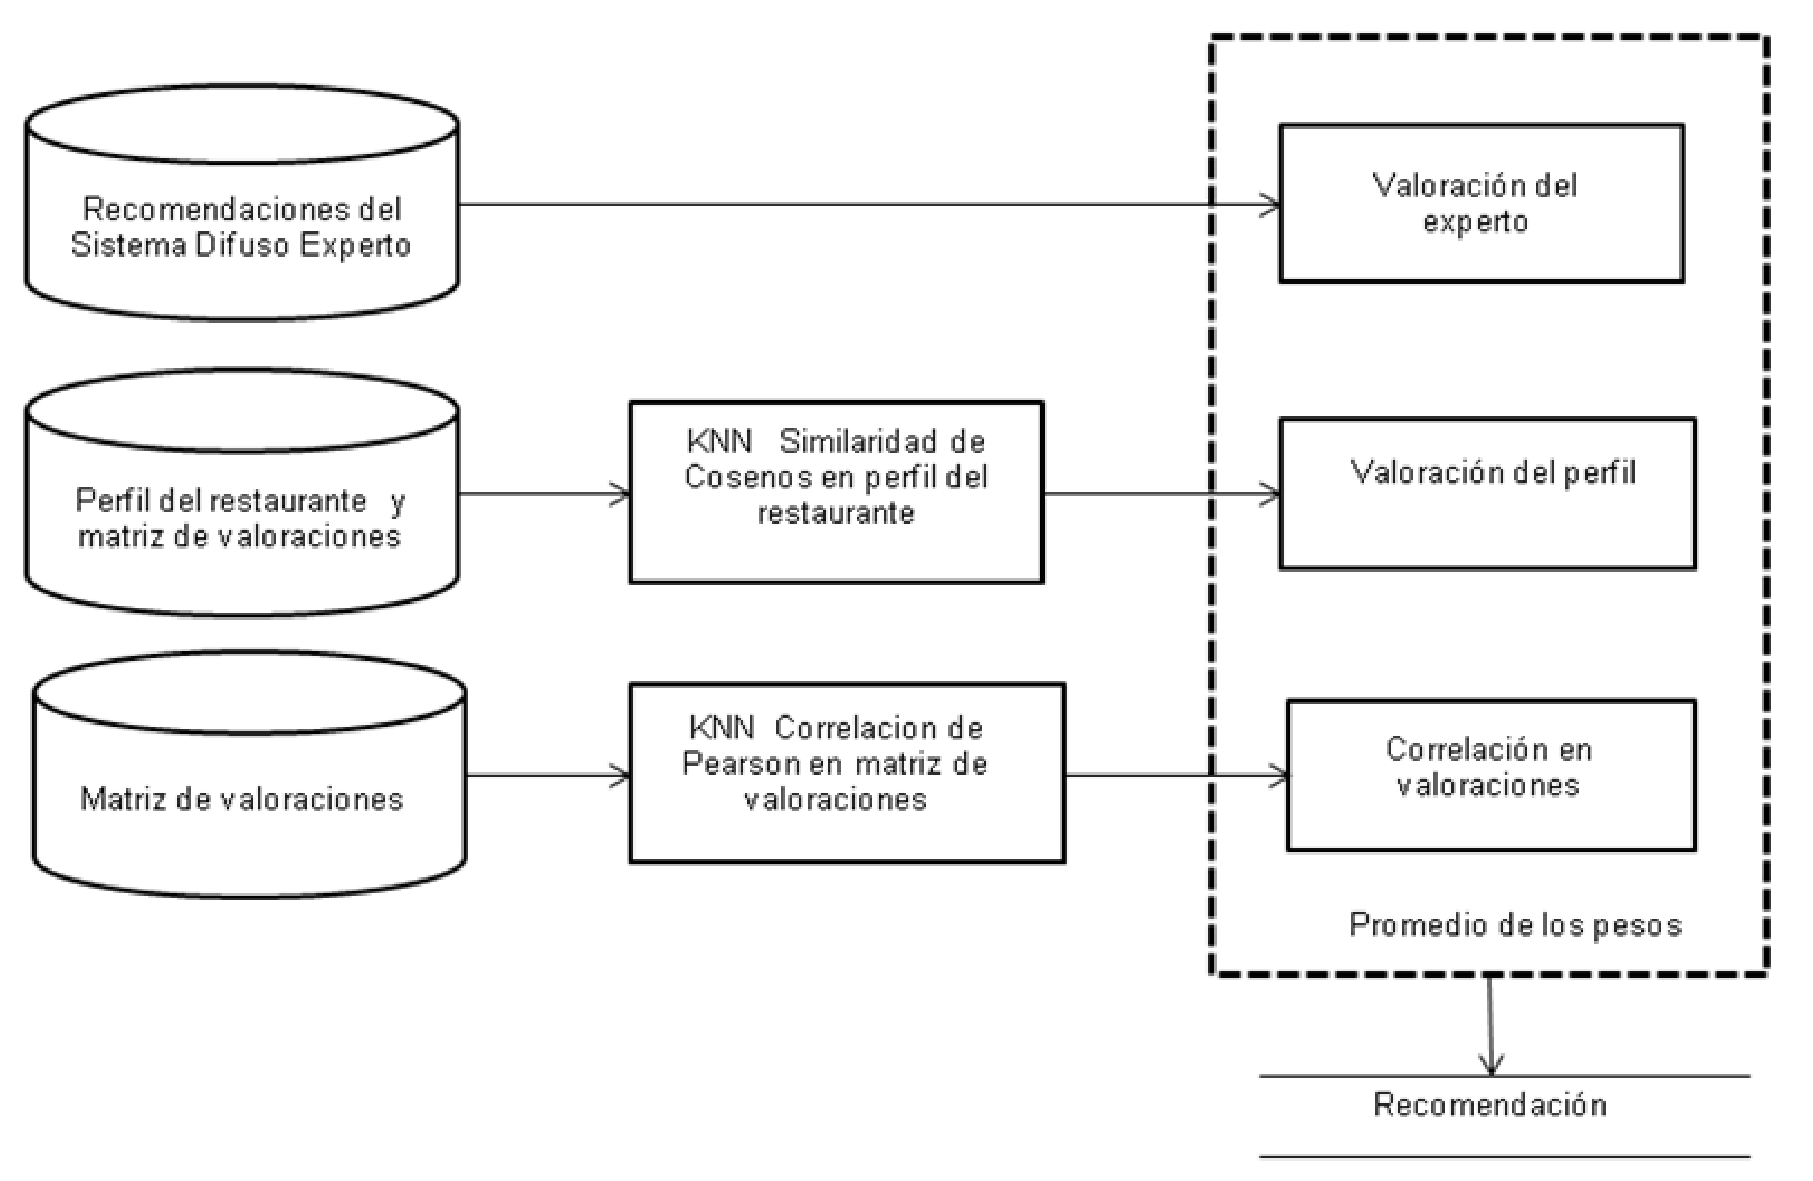
\includegraphics[width=0.9\textwidth]{./images/arquitectura2.pdf} 
} \caption{Arquitectura del sistema de recomendación.} 
\label{fig:arquitectura} 
\end{figure}


\chapter[Recomet: Recomendaciones de Tijuana]{Recomet}

En este capítulo se presenta un prototipo de sistema de recomendación de restaurantes para la ciudad de \textbf{Tijuana}, está basado en técnicas de lógica difusa y trabaja con un mecanismo de hibridación por pesos para generar recomendaciones.
 \paragraph*{}   
El sistema  recomendación híbrido está  compuesto de dos sistemas de  recomendación, uno colaborativo y uno basado en contenido.  En este sistema de recomendación, se ha empleado  un  mecanismo de \textbf{hibridación por pesos} \citep{Burke2002}. En este tipo de sistemas híbridos las técnicas de recomendación trabajan simultáneamente y para este caso, es un sistema difuso el que asigna los pesos a cada recomendación generada en el sistema para mostrar al usuario un promedio ponderado.
\paragraph{}
El  objetivo fue crear un sistema de recomendación que se pudiera aplicar en situaciones en donde a los usuarios les gustaría recibir recomendaciones sobre algún restaurante para comer. Implementar sistemas de recomendación de restaurantes, lugares turísticos o sitios de ocio resulta un poco complicado ya que presentan problemas que son considerables a la hora de generar recomendaciones \citep{PerezCordon2008}, enseguida se mencionan:

\begin{enumerate}
\item Muchos de los usuarios que interaccionan con el sistema, son \textbf{usuarios casuales} que nunca han usado el sistema de recomendación o que lo han usado de forma esporádica y no piensan utilizarlo de forma habitual. En el capítulo 2  se explicó que las técnicas clásicas de recomendación sufren del problema del nuevo usuario y por lo tanto no son capaces de generar recomendaciones cuando se encontraban en estas situaciones.
\item Un número importante de usuarios tendrá un \textbf{conocimiento basado en expectativas} sobre el servicio o producto que quieren recibir y es muy probable que no sepan expresar de forma clara y precisa las características del tipo de restaurante que desean visitar.
\item Es habitual que en este tipo de situaciones, existan usuarios que quieran recibir \textbf{recomendaciones puntuales} que no tengan nada que ver con lo que han hecho en el pasado. Por lo tanto, en estos casos, la información histórica no será relevante y no debería ser utilizada en la generación de recomendaciones. Por ejemplo, si un cliente desea celebrar un cumpleaños en un restaurante, es muy probable que sea un hecho puntual y que no quiera que se use la información de los restaurantes que le han gustado en el pasado para generar estas recomendaciones.
\end{enumerate}
Sin embargo, pese a este tipo de situaciones las recomendaciones generadas han demostrado ser aceptables.
\paragraph*{}
El prototipo en general fue desarrollado en Lenguaje \textbf{Python} \citep{Drake2000}, utilizando el framework \textbf{Django v1.2.} \citep{Django2008} para el desarrollo Web,  este framework permitió la implementación  sencilla de los algoritmos de recomendación integrados en el sistema (ver figura \ref{fig:arquitectura}), Django proporciona diversas funcionalidades que minimizan el esfuerzo de desarrollo. \textbf{Django} se complementa con el lenguaje de etiquetas \textbf{HTML} para el diseño de las páginas Web. 
La base de datos fue diseñada en \textbf{Visual Paradigm for UML v4.2} y creada en \textbf{PostgreSQL v9.0.} y un servidor Web para instalar la aplicación (Apache). 
En la  figura \ref{fig:p2} se muestra el prototipo final elaborado para pruebas y algoritmos, el principal objetivo de esta investigación.

\section{Aplicación}

En esta sección se describe cada función especificada en el prototipo, que inicia desde la parte administrativa hasta llegar a la recomendación para el usuario.

\subsubsection{Administración}
La parte inicial del sistema fue elaborar el sistema de administración basado en el modelo que ofrece el framework \textbf{Django},  fue sencillo de implementar por su funcionalidad, así, la administración del sistema se realiza desde la interfaz integrada en el framework, y se muestra en la figura  \ref{fig:p1}.

\begin{figure}[H]
\centering 
\framebox{
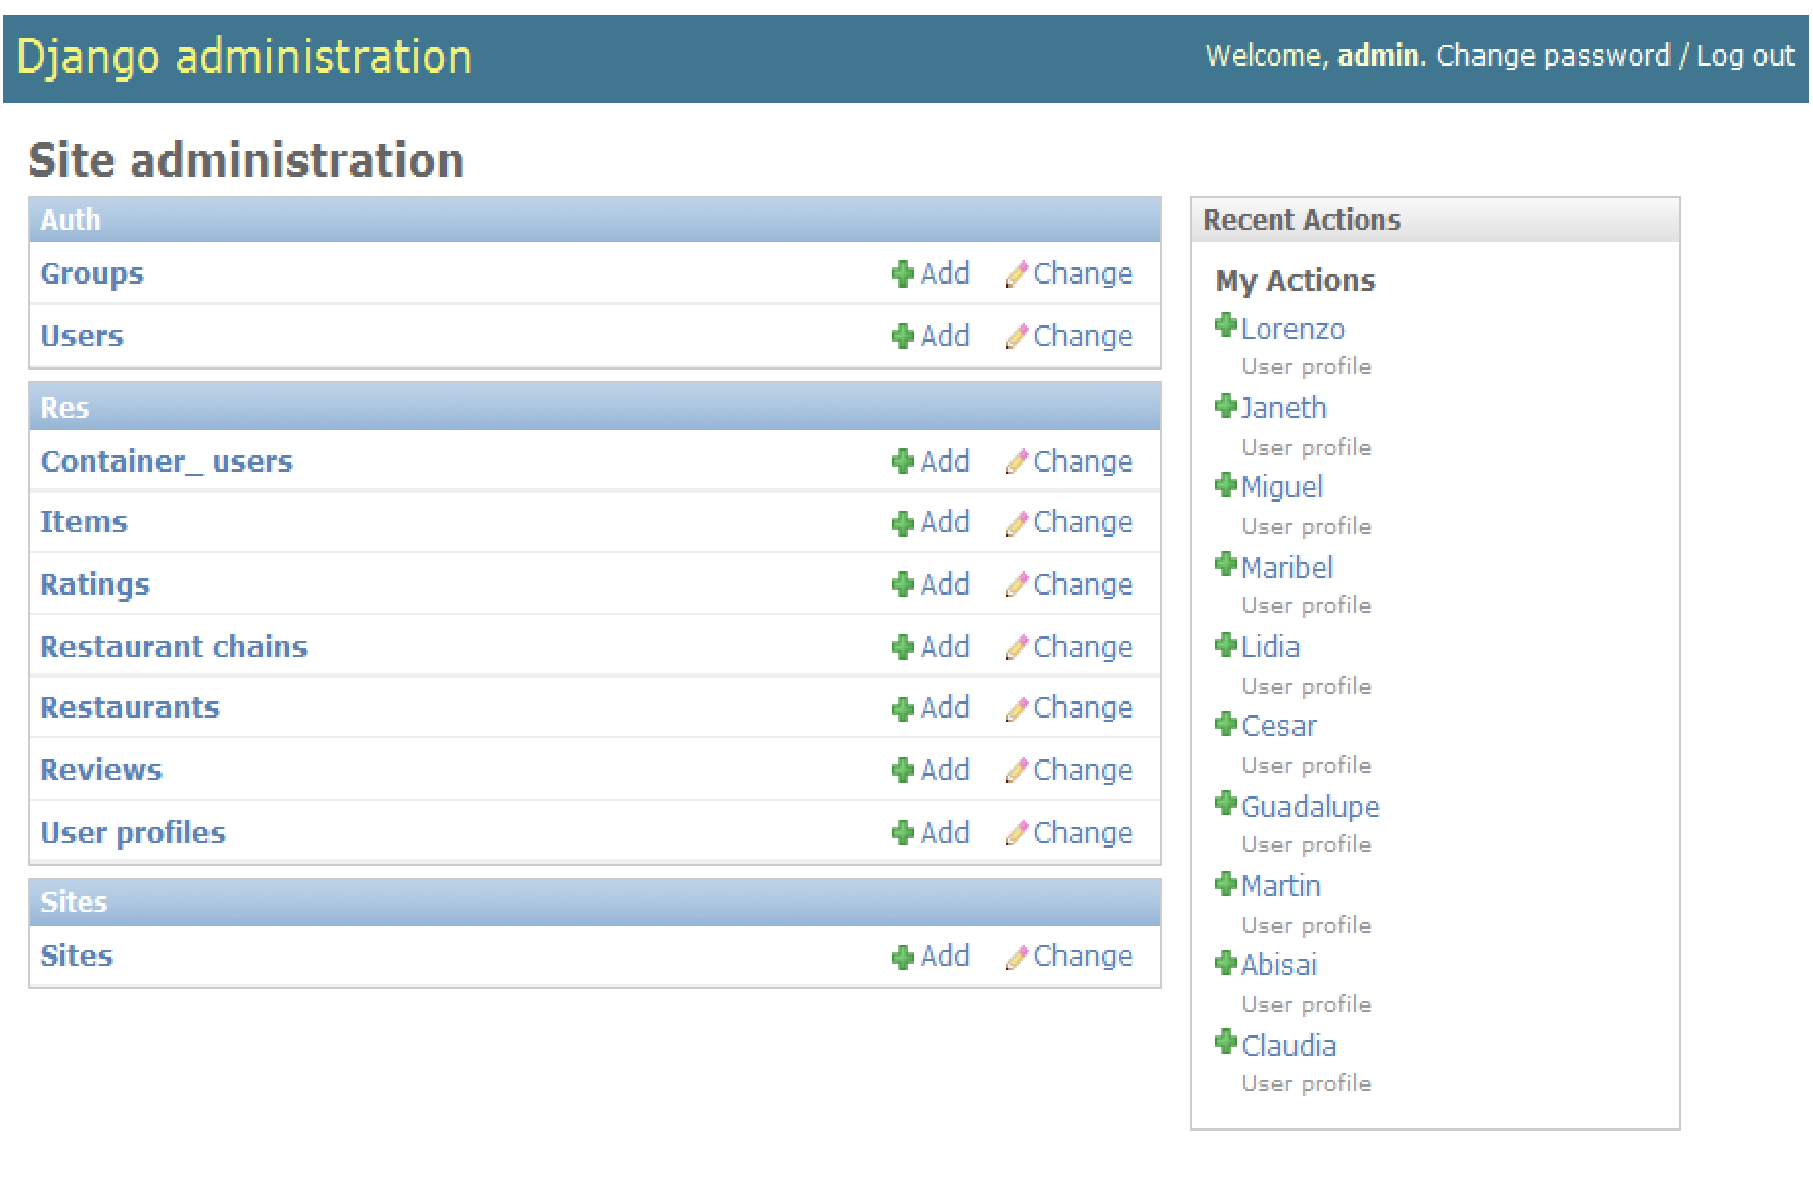
\includegraphics[width=0.7\textwidth]{./images/p1.pdf} 
} \caption{Administración del sitio.} 
\label{fig:p1} 
\end{figure}

Desde aquí la tarea de administrar el sitio se hace sencilla, en la figura \ref{fig:p1} se encuentran los \textbf{usuarios} (Users), los \textbf{grupos de usuarios} (Groups), los \textbf{contenedores}, los \textbf{restaurantes} (Items) de la base de datos, las \textbf{valoraciones} (Ratings) y todos los demás elementos que el usuario administrador debe controlar.  Desde aquí se manipula toda la información contenida en la base de datos, todos los detalles como fechas, horas, acciones de los usuarios, etcétera, ya que el administrador cuenta con todos los permisos para realizar cualquier transacción.

\subsubsection{Funcionalidad}

Para obtener recomendaciones, en primera instancia es importante recalcar que solamente los usuarios registrados obtendrán recomendaciones de este sistema como se observa en la figura \ref{fig:p2}, existe el \textbf{usuario invitado} (Guess) que solo podrá visualizar la información de los demás usuarios, las reseñas, perfiles de restaurantes y demás pero en ningún caso podrá agregar algún tipo de información.\\

\begin{figure}[H]
\centering 
\framebox{
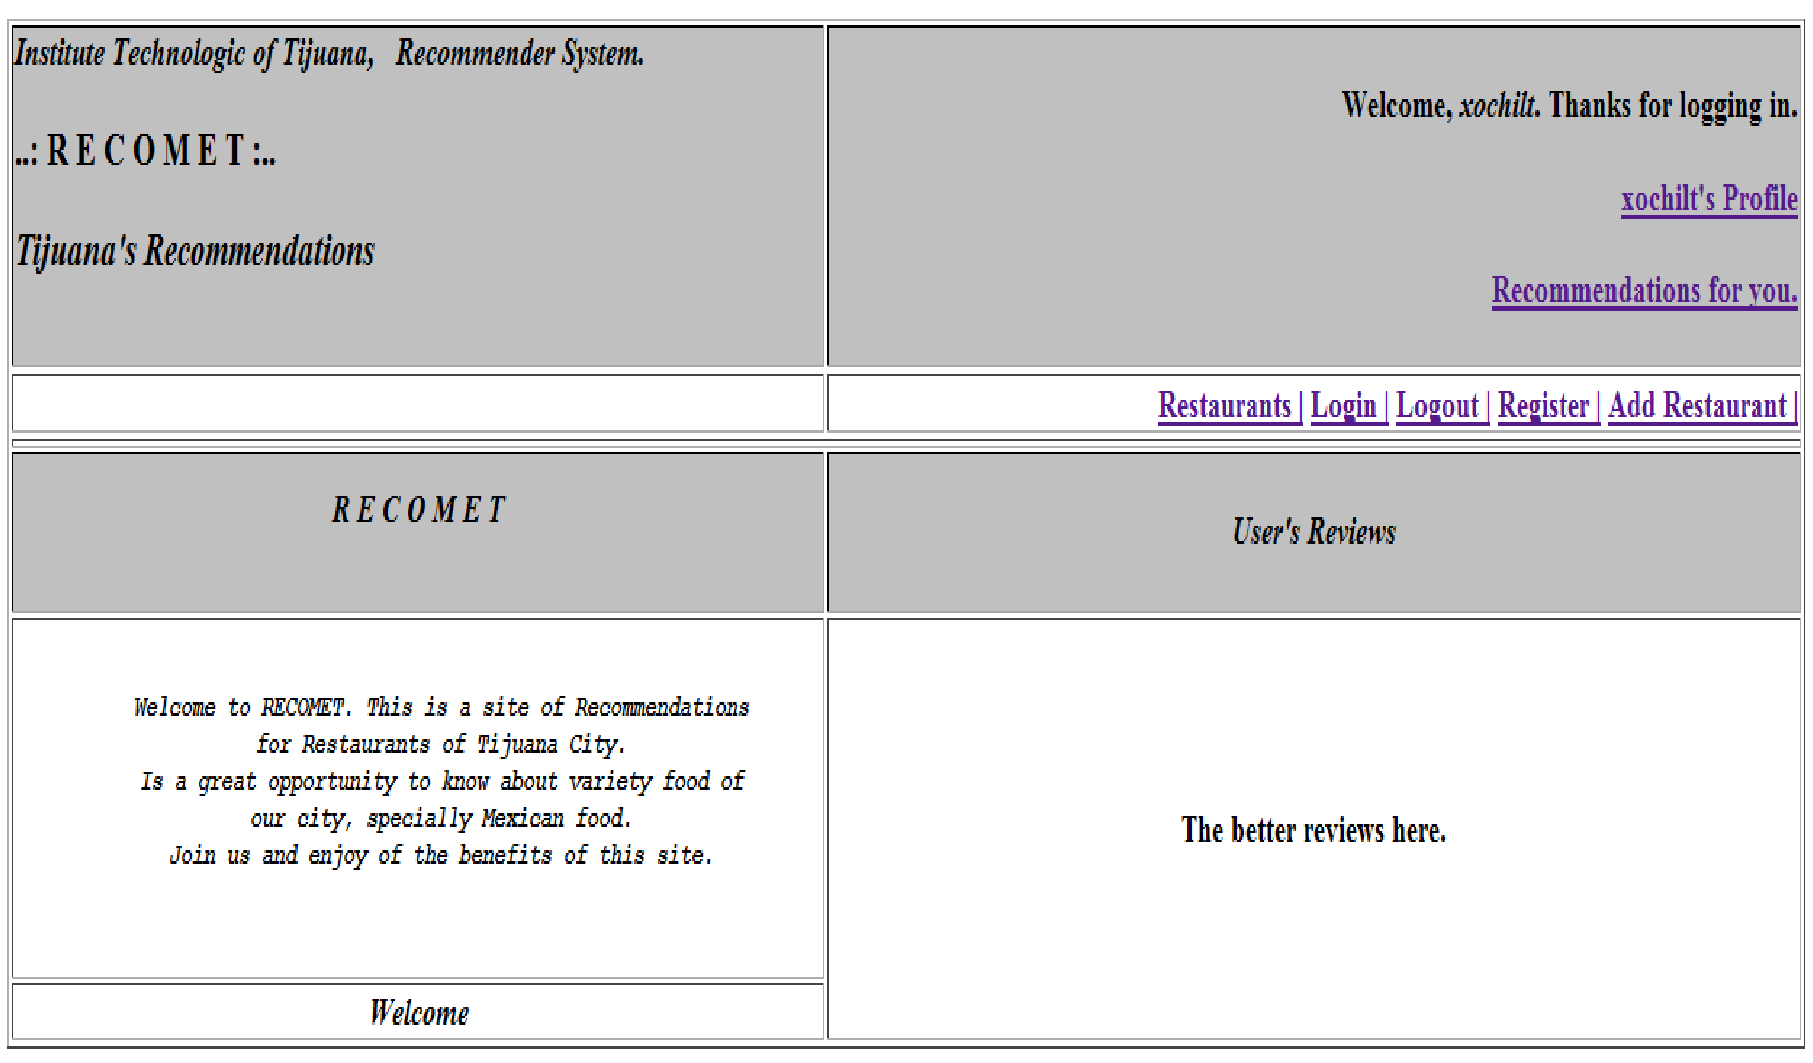
\includegraphics[width=0.8\textwidth]{./images/p2.pdf} 
} \caption{Pantalla principal del prototipo.} 
\label{fig:p2} 
\end{figure}

Para obtener los datos sobre un restaurante el usuario invitado debe pulsar sobre la opción \textbf{Restaurants} que aparece en la parte superior derecha de la pantalla principal. Una vez pulsada aparecerá la pantalla que se muestra en la figura \ref{fig:p3} donde se muestra información detallada en el perfil de cada restaurante.\\

\begin{figure}[H]
\centering 
\framebox{
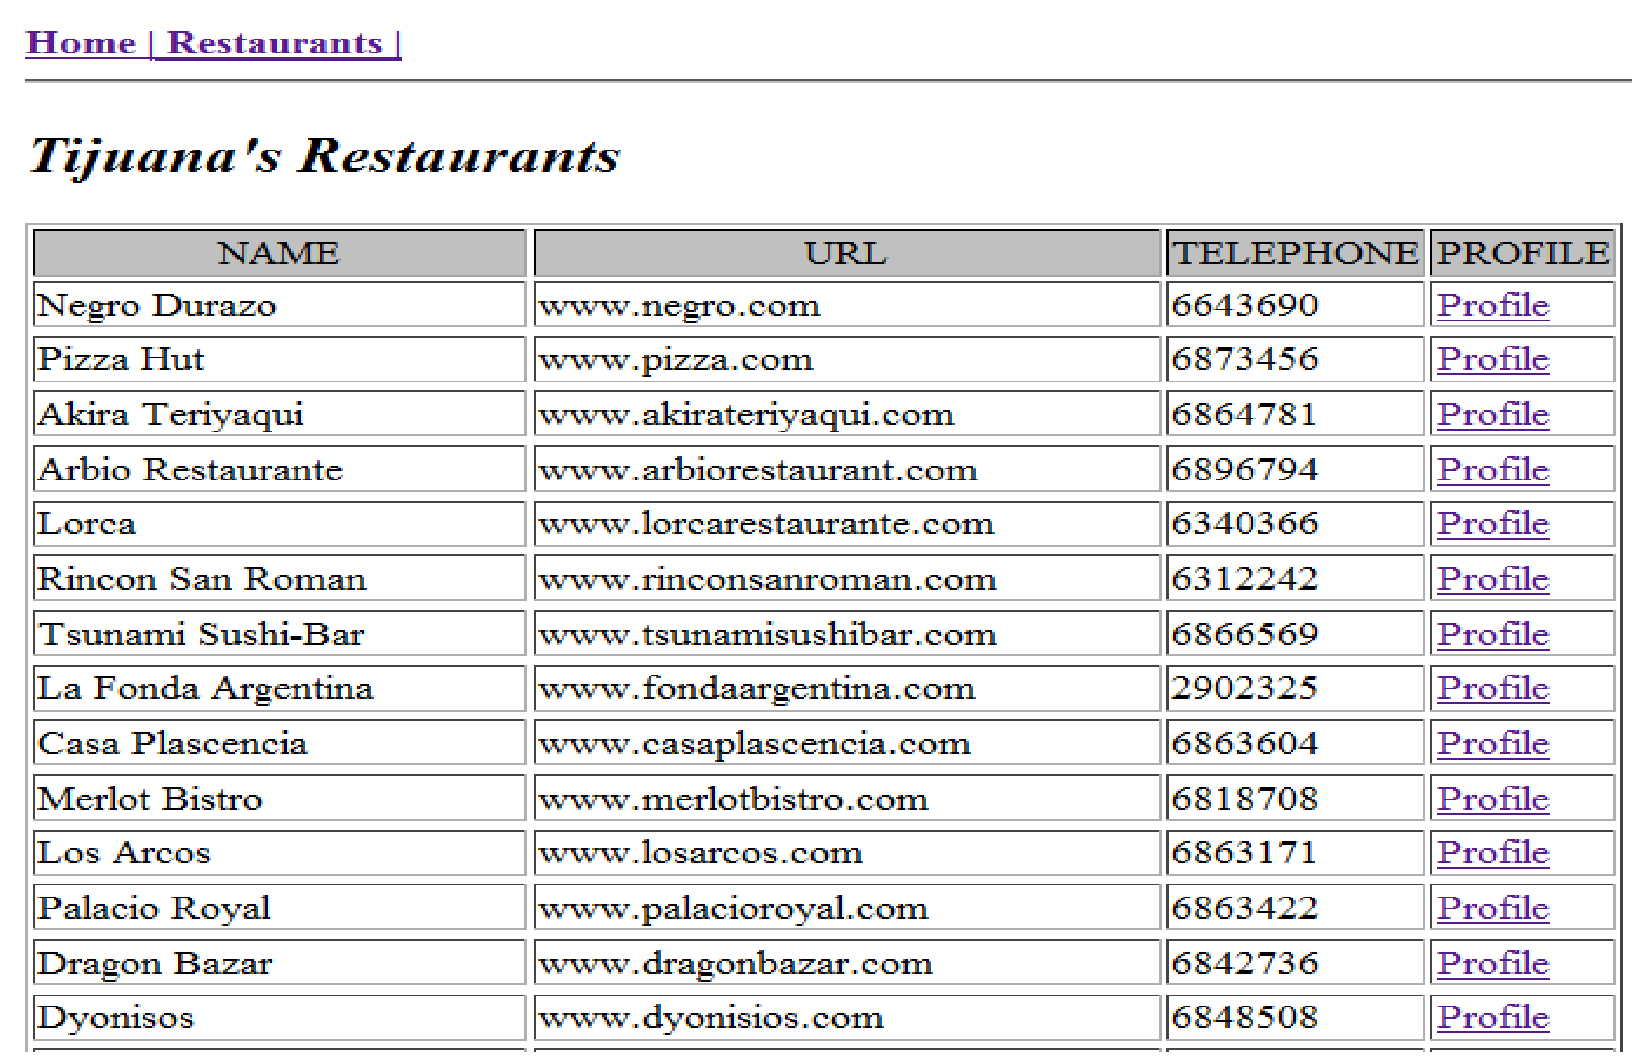
\includegraphics[width=0.8\textwidth]{./images/p3.pdf} 
} \caption{Listado de restaurantes para el usuario invitado.} 
\label{fig:p3} 
\end{figure}

Por otra parte, cuando el usuario esta registrado y es autentificado en el sistema aparecerá una sección de recomendaciones \textbf{(Recommendations for you)} que surgen en base a los algoritmos implementados en el sistema, esta es la respuesta a las preferencias que el usuario activo dio al sistema al realizar las valoraciones de los restaurantes, \textbf{las sugerencias} son mostradas como resultado del algoritmo colaborativo y el basado en contenido, así como la \textbf{recomendación del experto} basado en los parámetros explicados en el capítulo 3.
\paragraph{}
Se agregó la liga para acceder a la lista de restaurantes de la base de datos del sistema, en la figura \ref{fig:p4} se muestran los perfiles de cada restaurante, a su vez cada perfil tiene las opciones para  ver:
\begin{itemize}
\item Las valoraciones de otros usuarios que han votado ese restaurante.
\item Las reseñas que han agregado de su experiencia en ese restaurante.
\item Una ventana donde aparecerá la opción para votar ese restaurante.
\item Un botón para agregar el restaurante a una \textbf{lista de interés} (wishlist) si aún no lo ha visitado.
\end{itemize}

\begin{figure}[H]
\centering 
\framebox{
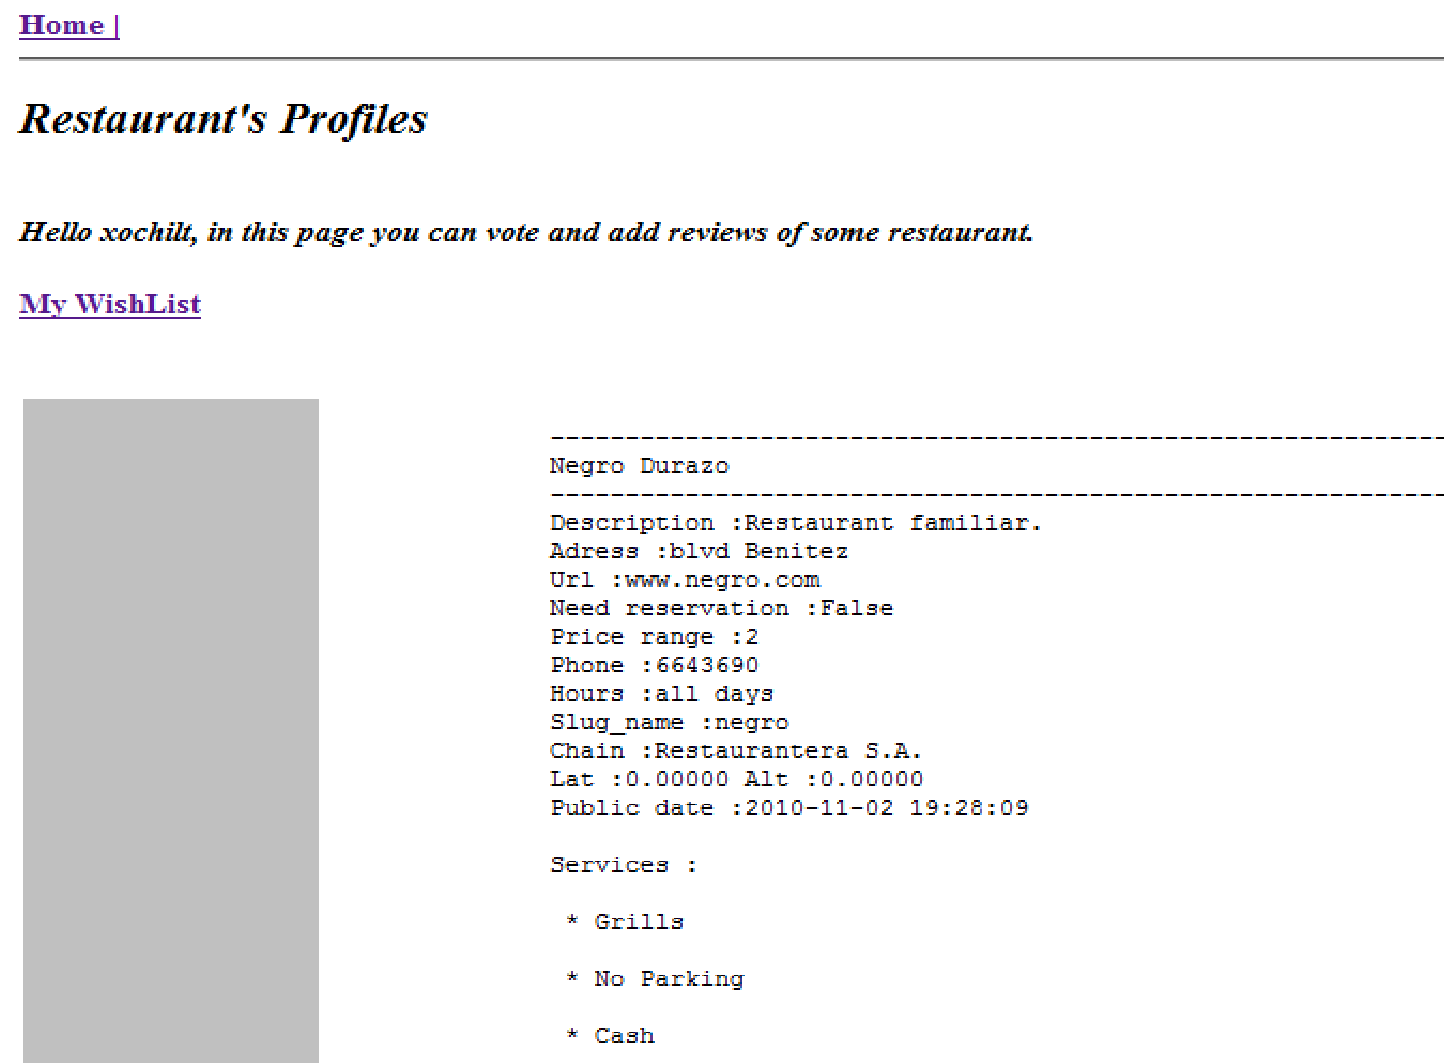
\includegraphics[width=0.8\textwidth]{./images/p4.pdf} 
} \caption{Información de perfiles de restaurantes para el usuario registrado.} 
\label{fig:p4} 
\end{figure}

Ciertamente, en la liga para \textbf{My Wishlist} mostrada en la parte superior izquierda de la página, se encuentran todos los restaurantes que el usuario activo ha seleccionado como restaurantes de su interés. La figura \ref{fig:p5} muestra la pantalla que aparece una vez que se ha pulsado en la liga.\\

\begin{figure}[H]
\centering 
\framebox{
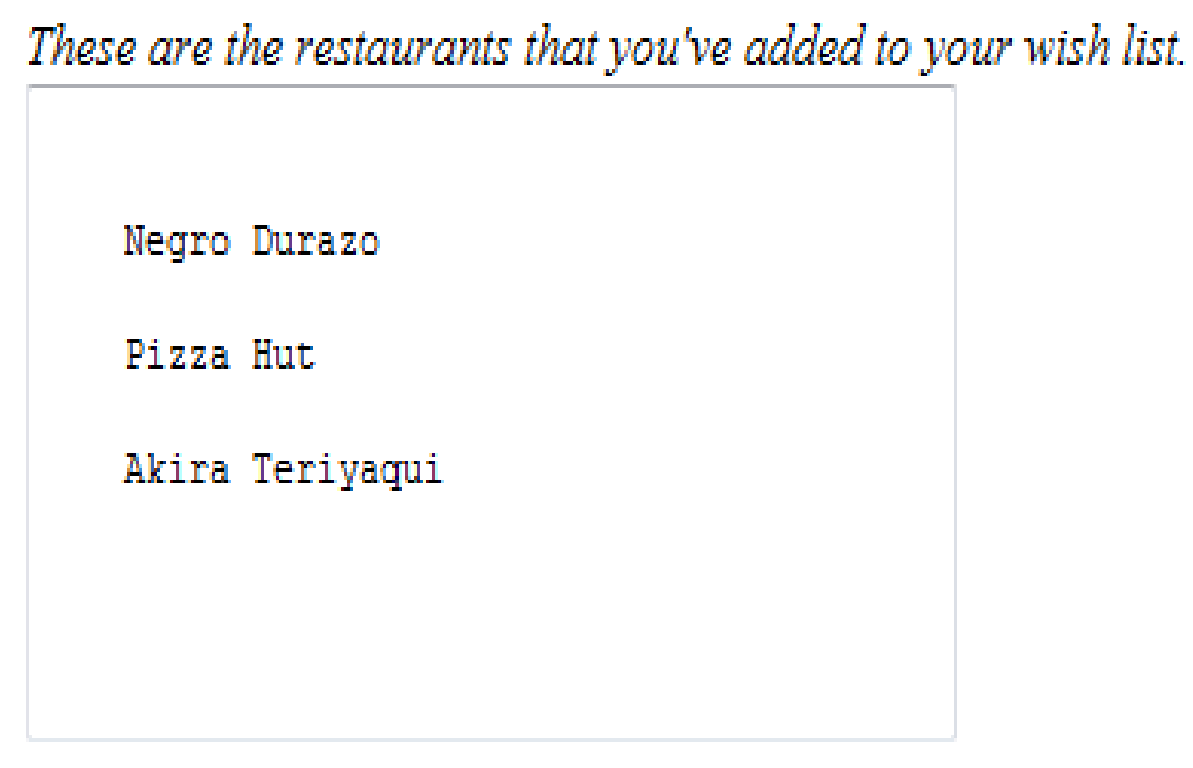
\includegraphics[width=0.8\textwidth]{./images/p5.pdf} 
} \caption{Lista de interés del usuario activo.} 
\label{fig:p5} 
\end{figure}

Desde la página principal también se observa la sección del perfil del usuario activo (\textbf{xochilt’s profile} para este caso), en esta sección se encuentra la descripción del perfil del usuario, se define en base a los datos proporcionados por él mismo, cabe mencionar que desde ahí el usuario tiene el control de los restaurantes que le interesan visitar, los que le gustan y los que le desagradan, también puede visualizar desde las ligas las valoraciones que ha asignado a los restaurantes que evaluó \textbf{(ratings)} y visualizar las reseñas que ha descrito sobre los restaurantes que ha visitado \textbf{(reviews)} ofreciendo también la posibilidad de agregar una nueva reseña \textbf{(add review)}, como se observa en la figura \ref{fig:p6}.

\begin{figure}[H]
\centering 
\framebox{
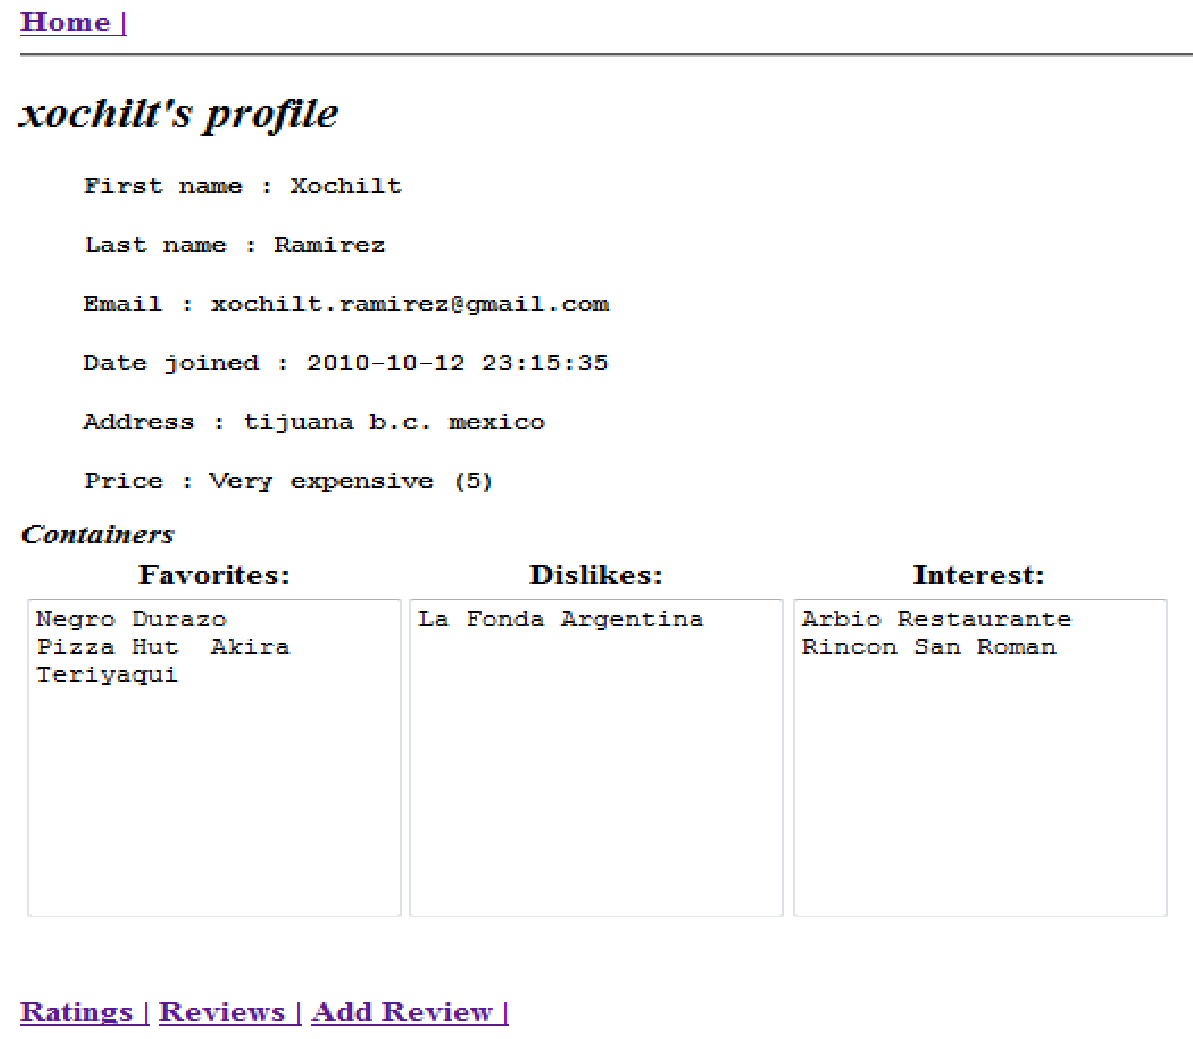
\includegraphics[width=0.8\textwidth]{./images/p6.pdf} 
} \caption{Perfil del usuario activo.} 
\label{fig:p6} 
\end{figure}

Otra opción que ofrece a los usuarios el sistema, es que pueden agregar restaurantes a la base de datos desde la liga \textbf{Add restaurant}  que se muestra en el menú principal (ver la figura \ref{fig:p2}).
\paragraph{}
Esta opción también es manejada desde el administrador, se pueden agregar restaurantes y sólo el administrador tiene permisos para aceptar los restaurantes agregados y eliminarlos si los datos están incorrectos, \textbf{Django administration} ofrece esta funcionalidad y se muestra en la figura \ref{fig:p7}.

\begin{figure}[H]
\centering 
\framebox{
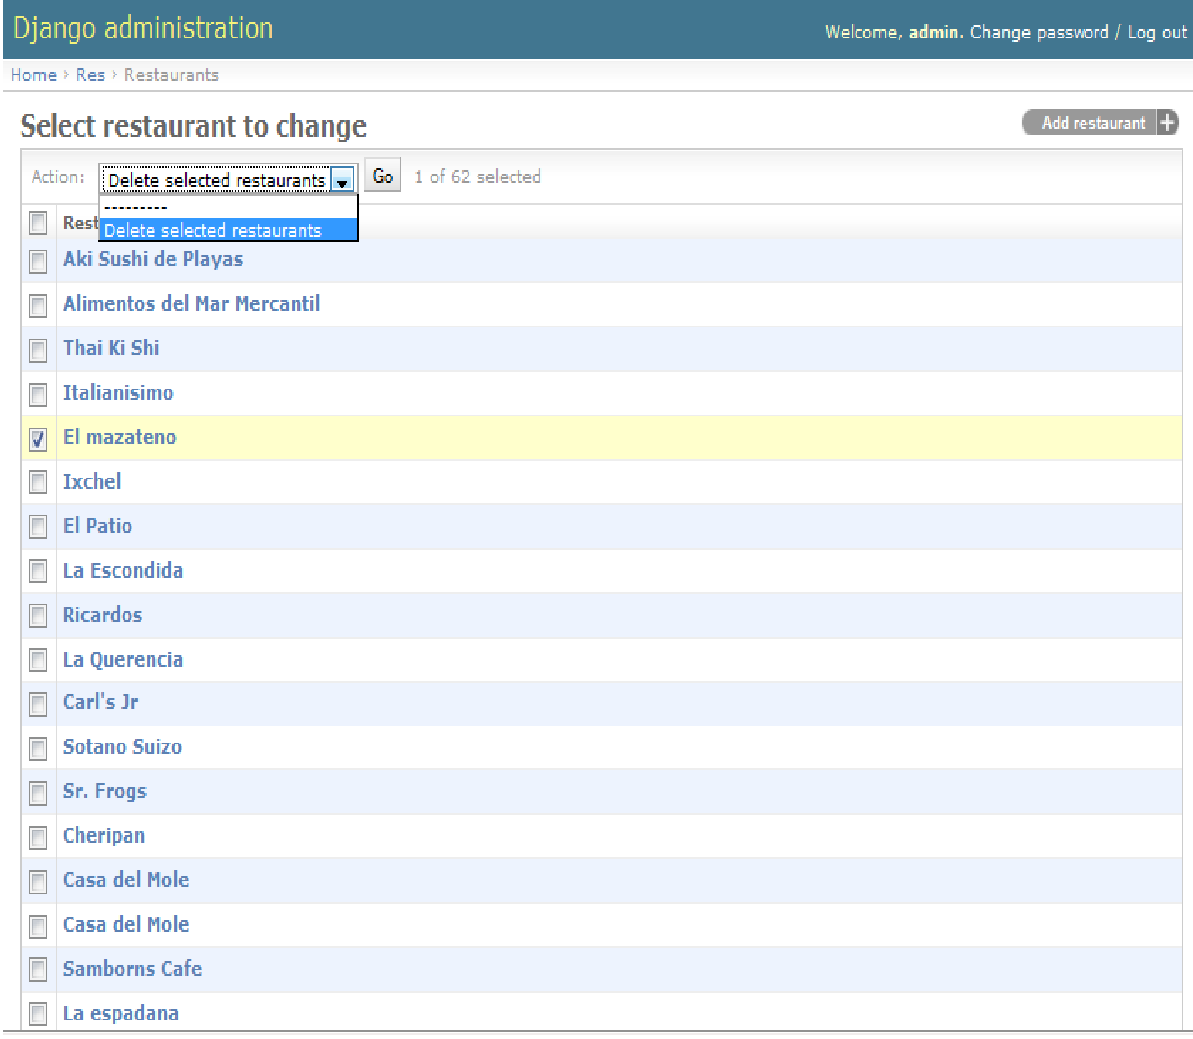
\includegraphics[width=0.8\textwidth]{./images/p7.pdf} 
} \caption{Manipulación de información de restaurantes desde el administrador.} 
\label{fig:p7} 
\end{figure}


\subsubsection{Módulo de filtrado colaborativo}

El módulo de filtrado colaborativo aplicado en el sistema \citep{PerezCordon2008} se resume en tres pasos:
\begin{enumerate}
\item El sistema \textbf{guarda un perfil} de cada usuario con sus evaluaciones sobre los restaurantes.
\item Se mide el \textbf{grado de similitud} entre los distintos usuarios del sistema en base a sus perfiles y se crean grupos de usuarios con características afines.
\item El sistema usará toda la información obtenida en las fases anteriores para \textbf{realizar las recomendaciones}. A cada usuario, le recomendará restaurantes que no haya evaluado y que hayan sido evaluados de manera positiva por el resto de miembros de su grupo.
\end{enumerate}

Gráficamente el sistema no muestra una sección para ver las recomendaciones basadas en filtrado colaborativo. Este proceso es interno y transparente al usuario así como los resultados obtenidos de esta técnica. Sin embargo, cabe mencionar que la operación de recomendación completa y de acuerdo a la arquitectura descrita en el capítulo 3,  se encuentra con la combinación de los tres métodos utilizados para generar recomendaciones al usuario activo. 
\paragraph{}
Esta sección se encuentra desde el menú principal (ver figura \ref{fig:p2}) en la liga \textbf{Recommendations for you}, donde se muestran las sugerencias.

\subsubsection{Módulo basado en contenido}

De igual manera que el módulo de filtrado colaborativo, el módulo basado en contenido está integrado en esta recomendación final. El proceso de este algoritmo se ha explicado en el capítulo 3, por lo tanto se reserva la explicación completa del proceso, sólo se explicará los detalles relevantes sobre este algoritmo en la aplicación.
\paragraph{}
Es importante mencionar que en este caso particular, el algoritmo ha trabajado con vectores binarios para la representación de las características de los restaurantes, el proceso es simple a la hora de comparar con la \textbf{similaridad de cosenos} para obtener  los restaurantes \textbf{más parecidos}, esta técnica también implementada en \citep{Burke2002}, mostró buenos resultados.  
\paragraph{}
Existen otras maneras como en \citep{Cristian2010} donde se muestra que la similaridad es basada en la repetición de palabras en un documento, utilizando principalmente la técnica de \textbf{Frecuencia de Términos y Frecuencia del Documento Inversa} (TF/IDF por sus siglas en inglés) \citep{Adomavicius2005} para obtener valores de aparición de cada palabra.  
Se puede comparar un documento Web con un perfil de restaurante tratándolos como documentos ambos,  pero en este sistema no se aplicó esta técnica porque los perfiles de los restaurantes son documentos pequeños y basarlos en las palabras que tienen mayor aparición sería inadecuado. En la figura \ref{fig:p8} se muestra el documento del perfil de restaurante que surge como una recomendación para el usuario activo, basada en los dos algoritmos.\\

\begin{figure}[H]
\centering 
\framebox{
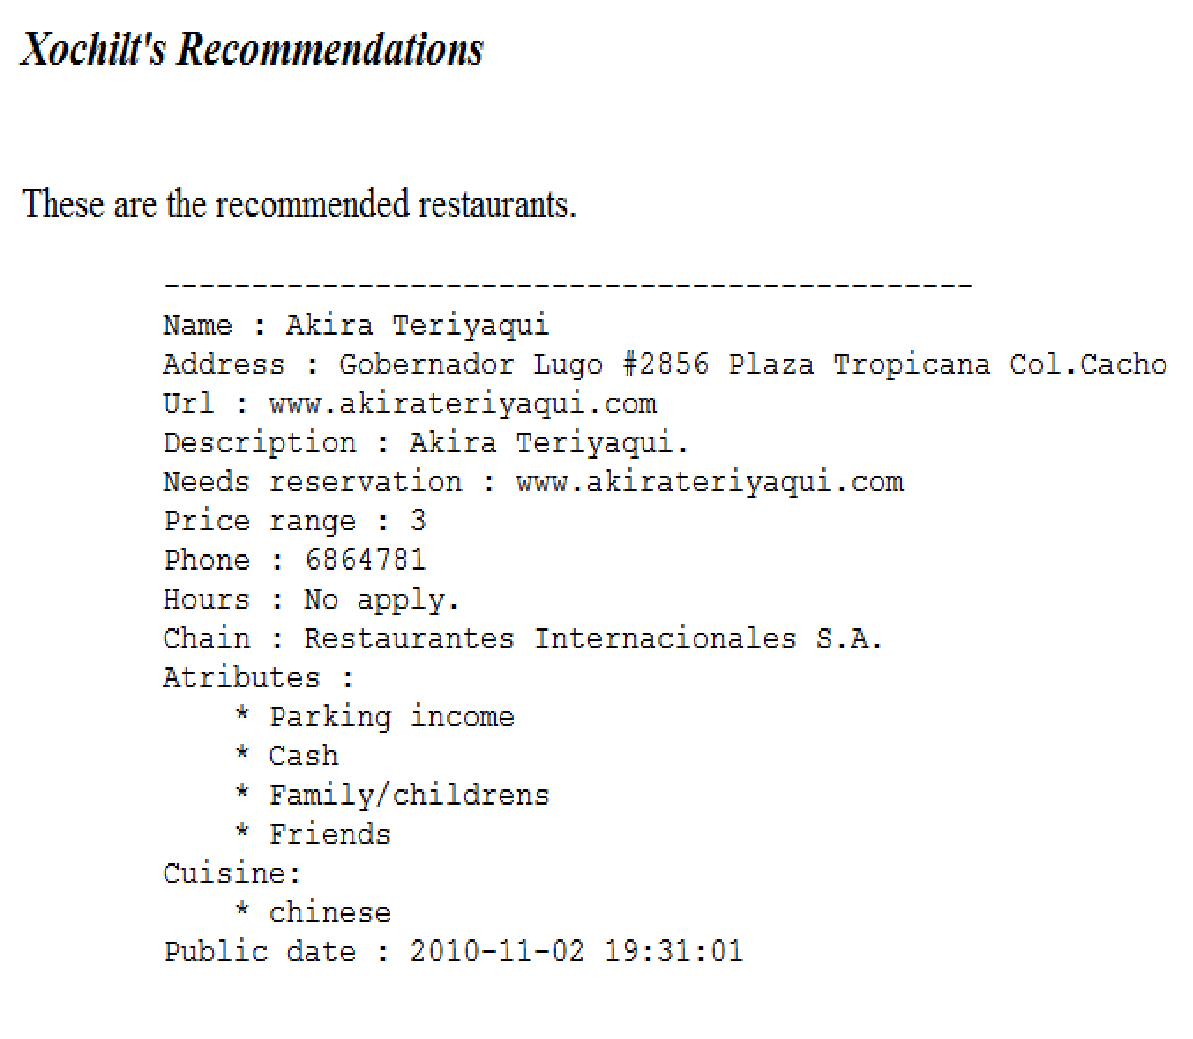
\includegraphics[width=0.8\textwidth]{./images/p8.pdf} 
} \caption{Recomendación final para el usuario activo.} 
\label{fig:p8} 
\end{figure}


\chapter[Métodos de evaluación]{Métodos de evaluación}

\section{Métricas}

Evaluar un sistema de recomendación debería ir mas allá de la \textbf{precisión} \citep{Adomavicius2005, Herlocker1991}, es lo más adecuado si se requiere que el sistema logre recomendaciones que realmente sean útiles al usuario. Por ejemplo, en informática una recomendación podría obtener un alto valor, pero en realidad ser una recomendación solo basada en la popularidad de los ítems, llegando a ser una sugerencia inútil.
\paragraph{}
Una de las métricas más convenientes para evaluar las recomendaciones es la idoneidad \citep{Herlocker2004} que incluye:
\begin{itemize}
\item \textbf{La cobertura} que mide el porcentaje de un conjunto de datos donde un sistema de recomendación es capaz de generar prediciones, 
\item \textbf{Indicadores de confianza} que pueden ayudar a los usuarios a tomar mejores decisiones.
\item \textbf{La tasa de aprendizaje} que mide la rapidez con que un algoritmo puede generar buenas recomendaciones.
\item \textbf{La novedad} que mide si una recomendación es una nueva posibilidad para un usuario.
 \end{itemize}
 
\paragraph{}
Por otra parte hay otros métodos estadísticos que sólo miden \textbf{la precisión} de los algoritmos en la recomendación, es evidente que una evaluación eficaz del rendimiento de los algoritmos de recomendación no es tarea sencilla. Primero porque diferentes algoritmos pueden ser mejores o peores dependiendo del conjunto de datos elegido. La mayoría de estos algoritmos están diseñados para el conjunto de datos de películas de \textbf{GroupLens} donde existe un número de elementos mucho menor al número de usuarios y votos. 
\paragraph{}
En una situación inversa el comportamiento puede diferir totalmente. El principio de este problema es que realmente no existe un método estandarizado que permita el logro de evaluaciones realmente significativas para estos algoritmos.
\paragraph{}
También si se consideran los objetivos del sistema de recomendación éstos pueden diversos. Un sistema puede diseñarse para estimar con exactitud la valoración que daría un usuario a un elemento, mientras otro puede tener como principal objetivo el no proporcionar recomendaciones erróneas. Es decir puede haber múltiples tipos de medidas: que las recomendaciones cubran todo el espectro de elementos del conjunto (cobertura), que no se repitan, que sean explicables. \\
Sin embargo el principal objetivo de un sistema de recomendación no es directamente cuantificable: \textbf{la satisfacción del usuario.} En muchos casos conseguir un error cuadrático menor al elegir un algoritmo u otro no es apreciado por el usuario.
\paragraph{}
Sin embargo hay muchos otros parámetros que pueden influir en esa satisfacción: la sensación de credibilidad que ofrezca el sistema, la interfaz de usuario, la mejora del perfil al incluir nuevos votos.  En cualquier caso las medidas de precisión pueden dar una primera idea de qué tan bueno es el algoritmo principal del sistema de recomendación. Existen dos tipos de métodos de evaluación \citep{GalanNieto1994}: \textbf{métodos estadísticos} y \textbf{métricas de decisión.}

\subsection{Métodos estadísticos}
El parámetro de evaluación más utilizado es el \textbf{Error Medio Absoluto} (MAE, por sus siglas en inglés), que mide la desviación de las recomendaciones predichas y los valores reales. A menor MAE mejor predice el sistema las evaluaciones de los usuarios. \\
El MAE sin embargo puede dar una idea distorsionada del algoritmo para el caso de sistemas que tienen como objetivo encontrar una lista de buenos elementos recomendables. El usuario tan solo está interesado en los \textbf{N} primeros elementos de la lista. El error que se cometa al estimar el resto es indiferente. 
\paragraph*{}
Tampoco es recomendable en sistemas en los que la salida deba de ser una decisión binaria de si/no. Por ejemplo, con una escala de 1 a 10 si el umbral esta situado en 5, utilizando MAE se obtendrá un mayor error al errar de 9 a 5 que al errar de 5 a 4, lo cual no es cierto a la hora de medir el error de salida. Sin embargo es un tipo de error estadísticamente muy sencillo de comprender. 
\paragraph{}
MAE Posee muchas variaciones, como el \textbf{Error Cuadrático Medio} que persigue penalizar los mayores errores o el \textbf{Error Absoluto Normalizado} que facilita la tarea de establecer comparaciones entre pruebas con diferentes conjuntos de datos.

\subsection{Métricas de decisión}

Evalúan la efectividad en las predicciones que realiza un sistema ayudando al usuario a seleccionar los elementos de mayor calidad, es decir, con qué frecuencia el sistema realiza recomendaciones correctas. Para ello asumen que el proceso de predicción es binario: o el elemento recomendado agrada al usuario o no lo agrada. Sin embargo en la práctica se plantea el problema de evaluar esto. 
\paragraph{}
Una posible solución es la de dividir el conjunto de datos en dos conjuntos, entrenamiento y test. Se trabaja con el conjunto de entrenamiento y posteriormente se evalúa el resultado comparando las recomendaciones proporcionadas con las del conjunto de test. Aun siendo a veces útil esta técnica, hay que tener en cuenta que los resultados dependen fuertemente del porcentaje de elementos relevantes que el usuario haya votado. 

\subsubsection{Precisión y Recuperación}

Es la más conocida de las métricas decisión, se utiliza en muchos tipos de sistemas de recuperación de información \citep{Herlocker2004, Sarwar2001, Basu1998, Billsus1998}. \textbf{Precisión} es la probabilidad de que un elemento seleccionado sea relevante y \textbf{Recuperación} es la probabilidad de que sea seleccionado un elemento relevante, aunque en los sistemas de recomendación la \textbf{relevancia} es algo totalmente subjetivo. Esta métrica es mas intuitiva, puesto que establecer que un sistema tiene una precisión del 90 por ciento significa que de cada 10 elementos recomendados 9 serán buenas recomendaciones, algo que no queda claro proporcionando valores de error cuadrático medio.

\subsubsection{Característica de Funcionamiento del Receptor (ROC por sus siglas en inglés)}

 Es otra medida muy utilizada que proporciona una idea de la potencia de diagnóstico de un sistema de filtrado \citep{Hanley1982, Herlocker2004}. Las curvas ROC dibujan la  \textbf{especifidad} (Probabilidad de que un elemento malo del conjunto sea rechazado por el filtro) y la  \textbf{sensitividad} (probabilidad de que un elemento bueno al azar sea aceptado). Si un elemento es bueno o malo viene dado por las valoraciones de los usuarios. Las curvas se dibujan variando el umbral de predicción a partir del cual se acepta un elemento. El área bajo la curva se va incrementando cuando el filtro es capaz de retener más elementos buenos y menos malos.

\section{Evaluación del sistema}
Para evaluar el sistema de recomendación de restaurantes se calculó el error en las recomendaciones con el método de \textbf{Raíz del Error Cuadrático Medio} (RMSE por sus siglas en inglés).  En el sistema se definió una matriz de valoraciones reales (ratings), \textbf{RMSE} permite calcular el error entre un vector de predicciones \textit{$\displaystyle v_{1}= [x_{1,1},x_{1,2},...x_{1,n}]$} y un vector de valoraciones reales \textit{$\displaystyle v_{2}= [x_{2,1},x_{2,2},...x_{2,m}]$} tomando estos vectores se calculó el error:

\begin{equation}
\displaystyle RMSE(v_{1},v_{2}) = \sqrt{\sum_{i=1}^{n}(x_{1,i}-x_{2,i})^{2}\over n}
\end{equation}

\paragraph{}
Para el primer experimento se utilizó una base de datos de 50 usuarios y 12 restaurantes.  La matriz utilizada se muestra en el apéndice A.
\paragraph*{}
Se probó el algoritmo de filtrado colaborativo y generó recomendaciones con error bajo. Es importante mencionar que constantemente se estuvieron comparando las pruebas usando dos distancias diferentes, la \textbf{distancia euclidiana} y la \textbf{correlación de Pearson}, la diferencia en los resultados fue en la mayoría de los casos, de decimales.\\


En la tabla \ref{tab:TableRecom} se muestran los resultados de la recomendación utilizando ambas distancias. Cabe mencionar que las mejores predicciones fueron calculadas con la \textbf{correlación de Pearson} y esto se refleja en los datos de la tabla.
\paragraph*{}
\begin{table}[H]
	\caption{Recomendaciones con filtrado colaborativo.} \begin{center}
\linespread{0.9}\selectfont
\begin{tabular}{>{\footnotesize}p{2.0in}>{\footnotesize}p{2.0in}}
\hline
Correlación de Pearson &  \\
\hline                    
Predicción  & Restaurante    \\
\hline             
4.99  & La vuelta del rodeo  \\
3.73  & Yogurt Place         \\
3.56  & La Querencia         \\
2.65  & Akira Teriyaqui      \\
\hline
Distancia euclidiana       & \\
\hline                    
Predicción  & Restaurante    \\
\hline
5.0   & La vuelta del rodeo  \\
4.0   & Sótano Suizo         \\
3.56  & Yogurt Place         \\
2.66  & La Querencia         \\
2.59  & Akira Teriyaqui      \\
\hline
\end{tabular}
\label{tab:TableRecom}
\end{center}
\end{table}

En un segundo experimento, se utilizó \textbf{RMSE} para calcular el error, con los mismos datos utilizados para generar las recomendaciones de las tablas anteriores. La tabla \ref{tab:RmsdPearson} muestra los resultados utilizando la \textbf{correlación de Pearson} y la \ref{tab:RmsdEuclidiana} los resultados utilizando la \textbf{distancia euclidiana}.
\paragraph*{}
\begin{table}[H]
	\caption{Raíz del Error Cuadrático Medio con correlación de Pearson.} \begin{center}
\linespread{0.9}\selectfont
\begin{tabular}{>{\footnotesize}p{1.0in}>{\footnotesize}p{1.0in}>{\footnotesize}p{1.0in}>{\footnotesize}p{1.0in}>{\footnotesize}p{1.0in}}
\hline                    
Usuarios & Num. de votos & Calificación & Predicción & RMSE\\
\hline             
10 & 6.2 & 3.794871795 & 3.179487179 & 0.877058019\\
20 & 6.35 & 3.746987952 & 3.156626506 & 0.911770421\\
30 & 6.3 & 3.873015873 & 3.380952381 & 0.776643163\\
40 & 6.225 & 3.714285714 & 3.291666667 & 0.827359541\\
50 & 6.18 & 3.609756098 & 3.141463415 & 0.838116355\\
\hline
\end{tabular}
\label{tab:RmsdPearson}
\end{center}
\end{table}


\begin{table}[H]
	\caption{Raíz del Error Cuadrático Medio con distancia euclidiana.} \begin{center}
\linespread{0.9}\selectfont
\begin{tabular}{>{\footnotesize}p{1.0in}>{\footnotesize}p{1.0in}>{\footnotesize}p{1.03in}>{\footnotesize}p{1.0in}>{\footnotesize}p{1.0in}}
\hline                    
Usuarios & Num. de votos & Calificación & Predicción & RMSE\\
\hline             
10 & 6.2 & 3.794871795 & 3.179487179 & 0.877058019\\
20 & 6.35 & 3.746987952 & 3.168674699 & 0.87811408\\
30 & 6.3 & 3.873015873 & 3.404761905 & 0.77151675\\
40 & 6.225 & 3.714285714 & 3.30952381 & 0.83094897\\
50 & 6.18 & 3.609756098 & 3.2 & 0.832275752\\
\hline
\end{tabular}
\label{tab:RmsdEuclidiana}
\end{center}
\end{table}

Los resultados obtenidos comprueban que en este caso la diferencia entre una distancia y otra es pequeña.
El error más grande lo refleja la \textbf{correlación de Pearson} con 20 usuarios, pero si se analizan las predicciones se observa que  las predicciones de las distancias tienen una diferencia mínima de 0.012048193, entonces puede decirse que las predicciones son aceptables en ambos casos.\\
Esta observación también se refleja en la gráfica de representación de los datos mostrada en la figura \ref{fig:graficarmsd}:
\paragraph*{}
\begin{figure}[H]
\centering 
\framebox{
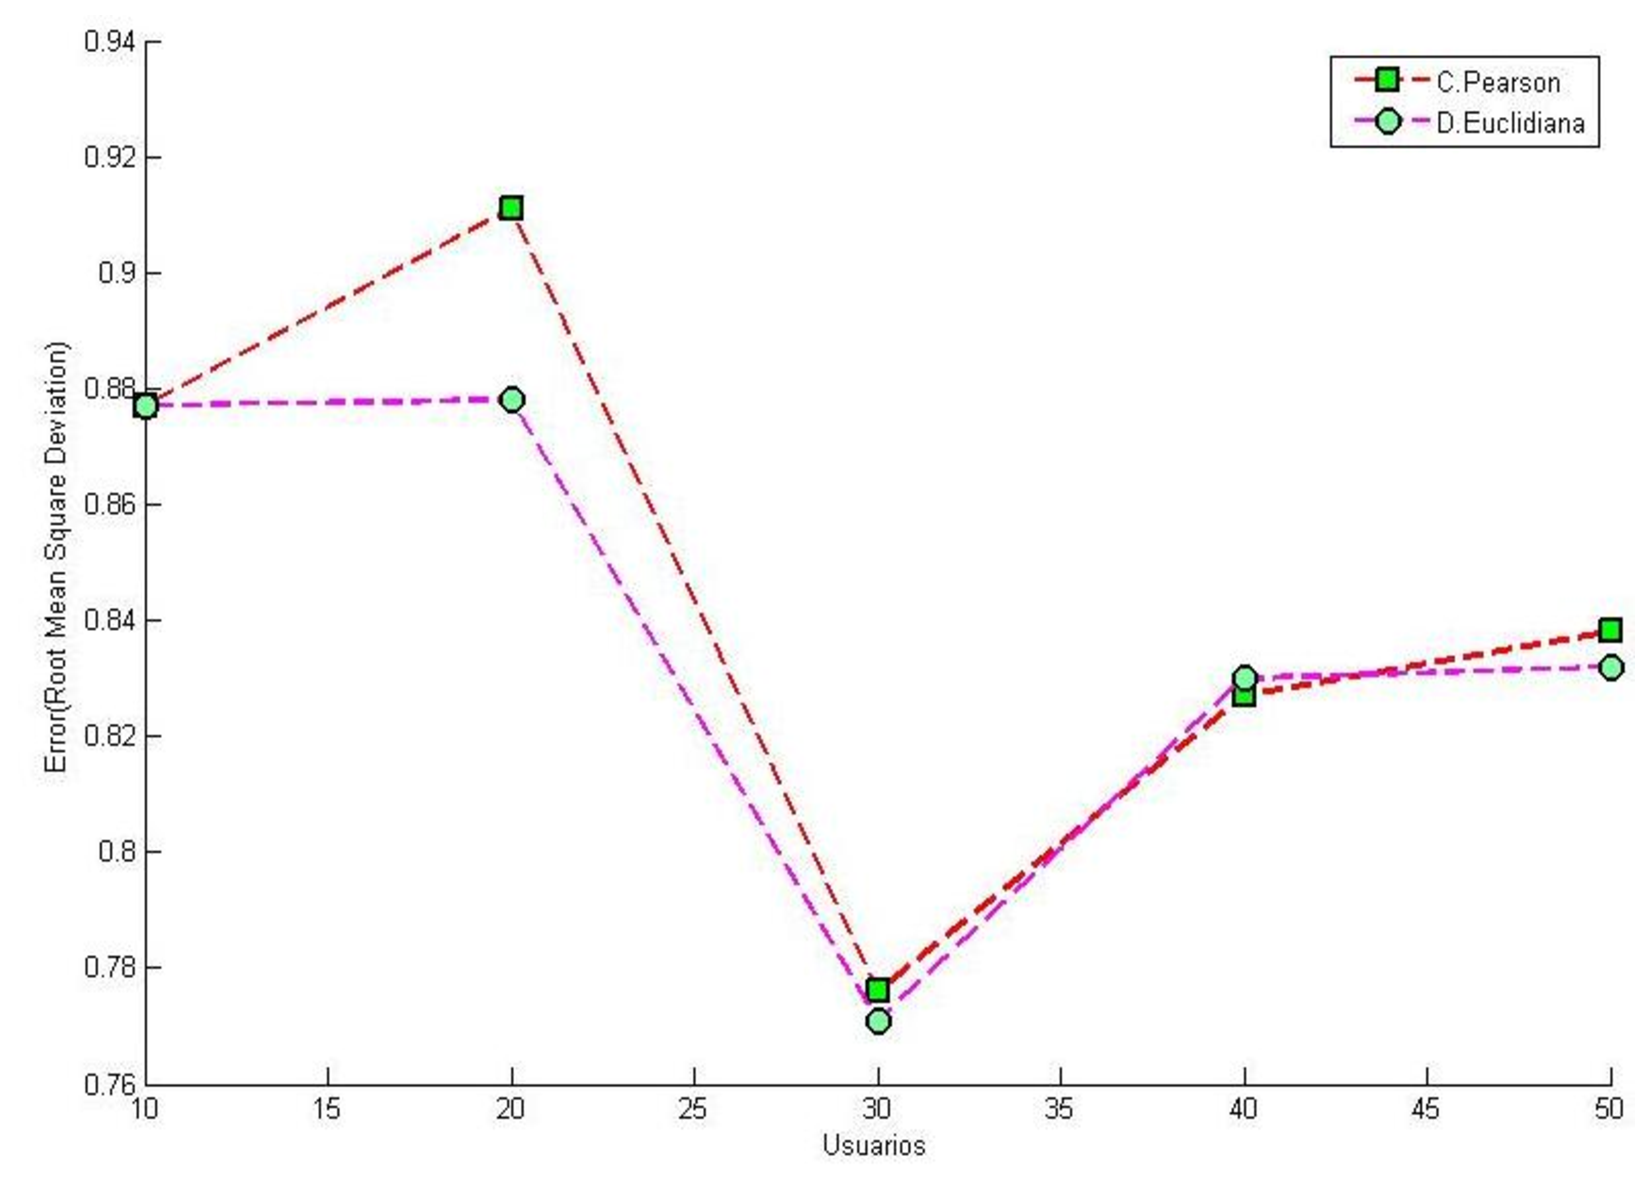
\includegraphics[width=0.8\textwidth]{./images/graficarmsd.pdf} 
} \caption{Gráfica de Raíz del Error Cuadrático Medio(RMSE).} 
\label{fig:graficarmsd} 
\end{figure}

La gráfica muestra que las variaciones entre una y otra no son significativas, sin embargo, la \textbf{correlación de Pearson} es más recomendada \citep{GalanNieto1994, Burke2002, Garciavaldez2009, Adomavicius2005}, es por esto que las recomendaciones están basadas en esta distancia. Partiendo del comportamiento de los datos, se puede decir que a partir de 30 usuarios el error en las predicciones empieza a disminuir. 
\paragraph{}
Posteriormente, se buscó obtener la \textbf{mejor} recomendación para el usuario utilizando los mismos datos que en los experimentos enteriores. Se hizo una prueba con los 30 usuarios, el promedio de votos por usuario fue 6. 
El objetivo fué comprobar si las recomendaciones obtenidas con dos operaciones de promedios resultaban diferentes, esto para identificar cuál podría mostrar un mejor resultado y optar por utilizar ese promedio en el sistema. 
\paragraph{}
Se experimentó con ambos promedios evaluando cada uno de los usuarios contenidos en la base de datos de pruebas y los resultados no variaron significativamente.
La prueba de evaluación nos dió los resultados mostrados en la tabla \ref{tab:promedios}, donde se observa una diferencia mínima y en algunos casos nula. Por lo tanto, se puede afirmar que ambos promedios son igualmente eficientes  para la recomendación en el sistema. 
\paragraph{}
Sin embargo, en la arquitectura del Sistema de Recomendación de Objetos de Aprendizaje \citep{Garciavaldez2009}, está definido el promedio ponderado, entonces el promedio que utilizó el sistema 
fue el mismo.
\paragraph*{}
Uno de los objetivos logrados en esta investigación fueron las recomendaciones con \textbf{mayor exactitud}, para este caso, basándonos en métodos estadísticos cuantificables. \\
Ciertamente, la precisión de una buena recomendación no da a los usuarios una experiencia \textbf{efectiva} y \textbf{satisfactoria}. Los sistemas de recomendación deben proporcionar no sólo precisión, sino también utilidad. Un sistema puede recomendar elementos muy populares  a usuarios tomando como métrica la popularidad pero esto no siempre resulta útil.
\paragraph*{}
Se podría en un futuro evaluar aspectos cualitativos del sistema, mediante métricas de decisión para obtener recomendaciones aceptables no sólo basadas en exactitud, sino también en aspectos cualitativos como la \textbf{satisfacción del usuario} que no puede ser minorizada si se considera que los sistemas de recomendación buscan sugerir al usuario como un \textit{amigo} lo haría.

\begin{table}[H]
	\caption{Comparación de las recomendaciones.} \begin{center}
\linespread{0.9}\selectfont
\begin{tabular}{>{\footnotesize}p{0.7in}>{\footnotesize}p{0.8in}>{\footnotesize}p{0.8in}>{\footnotesize}p{0.7in}>{\footnotesize}p{0.8in}>{\footnotesize}p{0.8in}}
\hline                    
Usuario & P.Ponderado & Promedio & Usuario & P.Ponderado & Promedio \\
\hline             
1    &    4.92    &    4.86  &  16  &    4.82    &    4.71 \\
2    &    4.89    &    4.86  & 17  &    4.66    &    4.58 \\
3    &    4.51    &    4.50  & 18  &    4.88    &    4.85 \\
4    &    4.90    &    4.86 &  19  &    4.86    &    4.85 \\
5    &    4.92    &    4.86  &  20  &    4.87    &    4.85 \\
6    &    4.89    &    4.84  &  21  &    4.89    &    4.85  \\
7    &    4.87    &    4.87  &  22  &    4.50    &    4.38 \\
8    &    4.91    &    4.86 &  23  &    4.86    &    4.86 \\
9    &    4.84    &    4.80 &  24  &    4.85    &    4.85 \\
10  &    4.87    &    4.84  &  25  &    4.54    &    4.61 \\
11  &    4.88    &    4.86  &  26  &    4.77    &    4.61 \\
12  &    4.57    &    4.35 &   27  &    4.83    &    4.71 \\
13  &    4.85    &    4.85 &   28  &    4.89    &    4.85 \\
14  &    4.86    &    4.86 &   29  &    4.85    &    4.85 \\
15  &    4.87    &    4.80 &   30  &    4.85    &    4.85 \\
\hline
\end{tabular}
\label{tab:promedios}
\end{center}
\end{table}




\chapter{Conclusiones y Trabajo Futuro}

\section{Conclusiones}

Las principales características del prototipo presentado son:
\begin{itemize}
\item Ofrece una mayor flexibilidad que los sistemas clásicos, ya que, permite a los usuarios que expresan sus preferencias mediante valoraciones lingüísticas.
\item Es capaz de realizar recomendaciones sólo si existe la información histórica o esta no se tiene que utilizar como es el caso del módulo basado en contenido. El uso de los algoritmos es necesario para recibir recomendaciones.
\item En el sistema se ha incluído un módulo basado en contenido para generar recomendaciones cuando no se requiera utilizar esta información histórica.
\item Es un prototipo que genera recomendaciones y su uso puede aprovecharse en  el sector turístico para facilitar la propagación de este tipo de herramientas en el mismo. 
\end{itemize}

\paragraph{}
Los sistemas de recomendación ofrecen recomendaciones personalizadas a sus usuarios, haciendo que el proceso de compra en tiendas virtuales  sea más rápido y personalizado. El objetivo es ofrecer a usuarios los productos que más les interesen o sean de su  \textbf{preferencia}. Para aprender estas preferencias los sistemas utilizan la información histórica del usuario, es decir, qué productos ha comprado o  evaluado. 
\paragraph{}
En este trabajo de investigación se explicó la arquitectura e implementación de un \textbf{sistema de recomendación de restaurantes híbrido.} Se utilizan algoritmos de filtrado colaborativo \citep{Segaran2007} y  basado en contenido para generar dos recomendaciones \citep{Burke2002}, una tercera recomendación es generada por un sistema difuso experto que toma parámetros identificados en cada restaurante para generar recomendaciones al usuario actual.
\paragraph{}
Para determinar las recomendaciones se involucran parámetros importantes a considerar para lograr una recomendación eficiente. Por un lado , el \textbf{ algoritmo de filtrado colaborativo} utiliza el mismo procedimiento que en otras investigaciones, aquí la diferencia la marca el conjunto de datos que se utilizan para obtener resultados. En este sistema se utilizó \textbf{información lingüística}, datos que de alguna manera son subjetivos y el sistema no está totalmente preparado para recibir este tipo de información, es posible que se necesite mayor granularidad en las funciones de membresía y agregar otros parámetros que también pueden ser importantes para un usuario al generar una recomendación.  
\paragraph{}
Por otro lado, las recomendaciones del \textbf{algoritmo basado en contenido} solamente estan basadas en la similaridad entre los restaurantes de base de datos,  aquí el algoritmo solo se basa en esta similaridad y no considera  la popularidad de cada restaurante entre los usuarios. Resultaría mucho mejor agregar este factor para mejorar el algoritmo, sin embargo, se obtienen recomendaciones aceptables.\\
\paragraph{}
Las técnicas de \textbf{lógica difusa} permiten implementar información imprecisa que maneja en la base de datos, de igual manera, esta información es recuperada por un sistema de inferencia que utiliza reglas difusas para asignar pesos a los algoritmos y generar una recomendación final mediante el promedio de pesos.
\paragraph*{}
Estos algoritmos están implementados en un prototipo que será utilizado para pruebas. Cada uno está generando recomendaciones de manera independiente, es decir, no influyen las recomendaciones de uno sobre el otro,  a su vez,  estas recomendaciones son mostradas al usuario a través de la interfaz diseñada en el prototipo.
\paragraph*{}
El método para evaluar el sistema fué la \textbf{Raíz del Error Cuadrático Medio (RMSE)} el cual permitió obtener las diferencias entre las predicciones de los algoritmos y las reales. Esto dió como resultado un error bajo considerando que el rango de valores es de 0 a 5 (ver tablas \ref{tab:RmsdPearson} y \ref{tab:RmsdEuclidiana}).
\paragraph{}
Los sistemas de recomendación han hecho progresos significativos en la década pasada, cuando numerosos sistemas  basados en el contenido, colaborativos y  métodos híbridos fueron propuestos y  han sido desarrollados. Sin embargo, a pesar de todos estos avances, la generación actual de sistemas de recomendación aún requiere nuevas mejoras para los métodos de recomendación más eficaz en una amplia gama de aplicaciones. 

\section{Trabajo Futuro}

Concluído el trabajo de investigación, se plantea en un futuro mejorarlo en los siguientes aspectos:
\begin{itemize} 
\item En la arquitectura considera tres módulos para generar recomendaciones al usuario activo. El \textbf{filtrado colaborativo} fue un buen algoritmo de recomendación, hizo predicciones con error bajo utilizando la \textbf{distancia euclidiana} y \textbf{correlación de Pearson}, estas distancias han sido muy utilizadas por otros investigadores por ser las que mejores resultados obtienen, sería una buena opción explorar otras y hacer más experimentos utilizando otras distancias.
\item En el caso del \textbf{algoritmo basado en contenido} se utilizó la \textbf{similaridad de cosenos}, fué sugerida como más efectiva para este tipo de algoritmos pero experimentar con otra opción para obtener una similaridad podría mostrar resultados inesperados.
\item El módulo de recomendaciones mediante el perfil de usuario podría agregarse en la arquitectura para generar recomendaciones basadas en el contenido del perfil de usuario, este caso podría utilizar \textbf{TF/IDF} (Frecuencia de Términos/Frecuencia del Documento Inversa) para analizar detalladamente el contenido de reseñas que el usuario hace sobre cada  restaurante que ha visitado.
\item Es conveniente agregar dentro del prototipo un \textbf{Sistema Geográfico Referenciado} como \citep{Espinilla2009} que permita la localización de cada restaurante de la ciudad y hacer recomendaciones basadas en la ubicación física del usuario activo, esto para tener más información sobre el usuario para generar recomendaciones que satisfagan sus expectativas.
\item La implementación de \textbf{RECOMET}, para obtener a partir del prototipo actual, un sistema de recomendación completamente funcional y de uso comercial en la ciudad.
\item Aplicar otras formas de obtención de información basándo las recomendaciones en una mayor cantidad de información de cada usuario.
\item Estudiar los \textbf{modelos de hibridación} más utilizados en otros sistemas con características similares a \textbf{RECOMET} con el objetivo de facilitar las recomendaciones y comparar con las obtenidas en el modelo actual del sistema.
\item Mayor flexibilidad en la definición de los \textbf{gustos} y \textbf{preferencias} del usuario, refinando el sistema para trabajar con mas datos lingüísticos.
\item Optimización de los sistemas difusos implementados para generar recomendaciones.
\item Evaluar el sistema utilizando \textbf{métricas de decisión} (Precisión y Recuperación, Idoneidad, ROC, etcétera) con el objetivo de mejorar la satisfacción del usuario en el sistema.
\item Crear una base de datos de restaurantes con información real ya que sólo se obtuvo información basada en Internet pero no fué comprobada su autenticidad.
\end{itemize}
Son muchas las mejoras que se pueden hacer al sistema, sin embargo, habría que analizar cuáles son las más convenientes y viables para su implementación, podría darse el caso que alguna empeore los resultados en las recomendaciones como el uso de otras distancias para obtener similaridad entre usuarios y restaurantes.

%\bibliographystyle{plain}
%\bibliography{biblio}
\begin{thebibliography}{99}

\bibitem{Acilar2009}  Acilar, A., Merve A.; Ahmed (2009). \textit{A collaborative filtering method based on artificial immune networks. Expert Sistems with applications,} 161.
\bibitem{Willey 2000}  Wiley, D. A. (2000). \textit{Connecting learning objects to instructional design theory: A definition, a metaphor, and a taxonomy. The Instructional Use of Learning Objects}, Bloomington: Association for Educational Communications and Technology, (pp. 3(23).



\end{thebibliography}

\appendix

\chapter{Programación del sistema}

\lstset{language=python}
\begin{lstlisting} [basicstyle=\scriptsize]	

#MODELO DE BASE DE DATOS EN DJANGO V1.2

from django.db import models
from models import *
import datetime
from django.utils.translation import get_date_formats
from django.utils import formats
from django.forms import ModelForm, TextInput, widgets
from django import forms
from django.contrib.auth.models import User

PRICE=(
    (1, 'very cheap'),
    (2, 'cheap'),
    (3, 'more and less'),
    (4, 'expensive'),
    (5, 'very expensive')
    )

LANG = (
    ('es', 'Espanol'),
    ('en', 'English'),
    ('fr', 'French'),
    ('jp', 'Japanese'),
   )
   
RATING=(
    (1, 'Awful'),
    (2, 'Bad'),
    (3, 'So so'),
    (4, 'Good'),
    (5, 'Excelent')
    )

class Cuisine(models.Model):
    cuisine = models.CharField(max_length=28)
    def __unicode__(self):
        return self.cuisine

class Atribute_Group(models.Model):
    group = models.CharField(max_length=32, null=True)
    def __unicode__(self):
        return self.group

class Atribute(models.Model):
    group = models.ForeignKey(Atribute_Group) 
    value = models.CharField(max_length=32)
    def __unicode__(self):
        return self.group.group
    
class RestaurantChain(models.Model):
    is_international = models.BooleanField()
    name = models.CharField(max_length=128)
    speciality = models.CharField(max_length=128)
    year_founded = models.PositiveSmallIntegerField(null=True)
    locations_worldwide = models.PositiveSmallIntegerField(null=True)
    
    def __unicode__(self):
        return self.name
    
class Recommender_rule(models.Model):
    rule = models.TextField()
    def __unicode__(self):
        return self.rule
    
class Item(models.Model): 
    rule = models.ForeignKey(Recommender_rule, null=True)
    def __unicode__(self):
        return self.rule.rule

class Restaurant(models.Model):
    item = models.OneToOneField(Item, unique=True) #Llave primaria
    name = models.CharField(max_length=255)
    address = models.TextField(max_length=512, null=True)
    description = models.TextField()
    needs_reservation = models.BooleanField()
    price_range = models.IntegerField(max_length=2,choices=PRICE, null=True)
    url = models.CharField(max_length=512, null=True)
    phone = models.CharField(max_length=18, null=True)
    hours = models.CharField(max_length=50, null=True)
    slug_name = models.SlugField(max_length=18, null=True)
    chain = models.ForeignKey(RestaurantChain, null=True)
    atribute = models.ManyToManyField(Atribute)
    cuisine =  models.ManyToManyField(Cuisine)
    lat = models.DecimalField(max_digits=8, decimal_places=5, null=True) 
    alt = models.DecimalField(max_digits=8, decimal_places=5, null=True)
    pub_date =  models.DateTimeField()    
    def __unicode__(self):
        return self.name

class Container(models.Model):
    container_name = models.CharField(max_length=64) 
    is_public = models.BooleanField()
    def __unicode__(self):
        return self.container_name

class Rating_Dimension(models.Model):
    dimension_name = models.CharField(max_length=64)
    priority = models.IntegerField(null=True)
    
    def __unicode__(self):
        return self.dimension_name

class UserProfile(models.Model):
    user = models.OneToOneField(User, unique=True)

    adress = models.CharField(max_length=512) 
    price = models.IntegerField(max_length=1,choices=PRICE)
    atribute = models.ManyToManyField(Atribute)
    cuisine = models.ManyToManyField(Cuisine)

    container = models.ManyToManyField(Container, through='Container_User')
    ratings = models.ManyToManyField(Item, through='Rating', related_name='ratings')
    reviews = models.ManyToManyField(Item, through='Review', related_name='reviews')
  
    def __unicode__(self):
        return self.user.first_name

class Rating(models.Model):
    id_item =  models.ForeignKey(Item) 
    user = models.ForeignKey(UserProfile) 
    id_dimension = models.ForeignKey(Rating_Dimension, null=True)
    date = models.DateTimeField()
    rating = models.PositiveSmallIntegerField(choices=RATING)
    interested = models.BooleanField()
    def __unicode__(self):
        return self.user.user.first_name
    
class Review(models.Model):
    item_reviewed = models.ForeignKey(Item)
    user = models.ForeignKey(UserProfile) #id_user
    title = models.CharField(max_length=128)
    review = models.TextField()
    status = models.PositiveSmallIntegerField(null=True)
    review_time = models.DateTimeField()
    #review_time = datetime.datetime.now()
    helpful_yes = models.IntegerField(max_length=128, null=True)
    helpful_no = models.IntegerField(max_length=128, null=True)
    language = models.CharField(max_length=2, choices=LANG)
    
    def __unicode__(self):
        return self.title
    
class Friends(models.Model):
    user = models.ForeignKey(UserProfile, related_name='id_user')
    id_friend = models.ForeignKey(UserProfile, related_name='friends') 
    time_added = models.DateTimeField(null=True)
    
    def __unicode__(self):
        return self.user.user.first_name

class Container_User(models.Model):
    id_container =  models.ForeignKey(Container)  
    user = models.ForeignKey(UserProfile)
    id_itemid_item = models.ForeignKey(Item)
    
    def __unicode__(self):
       return self.user.user.first_name

class Tag(models.Model):
    tag = models.CharField(max_length=18)
    id_item = models.ForeignKey(Item) 
    
    def __unicode__(self):
        return self.tag


#ALGORITMO DE FILTRADO COLABORATIVO.

def matuser(id):  
    r = Rating.objects.values_list('user','id_item','rating').filter(interested=0)
    list_t=[]
    if(r):
        for i in r:
            list_t.append(i)
    
    us_it = dict([(t[0],{}) for t in list_t])
    for t in list_t:
        us_it[t[0]][t[1]]=float(t[2])
    
    pearsonCorrelation = topMatches(us_it,id) 
    pr = getRecommendations(us_it,id,similarity=sim_pearson)
    der = getRecommendations(us_it,id,similarity=sim_distance)
    
    l_item=[]
    if len(pr)>3:
     for i in range(3):
        item = Restaurant.objects.get(item=pr[i][1])
        l_item.append(item)
    else:
     for i in range(len(pr)):
        item = Restaurant.objects.get(item=pr[i][1])
        l_item.append(item)
    return pr 


#ALGORITMO BASADO EN CONTENIDO.

def vecprofiles(id):
    rat2 = Rating.objects.all().filter(user=id,rating=5,interested=0)
    
    val2=[]
    if(rat2):       
        [val2.append(i.id_item.id) for i in rat2]
    
    profile = []
    for i in val2:
        ida2 = []
        idc2 = []
        res2 = []
        
        r = Restaurant.objects.get(item=i)    
        c1 = r.item.id
        
        binp2 = [0,0,0,0,0]
        for i in range(5):
            if(i==r.price_range):
                binp2[i]=1
            elif(r.price_range==5):
                binp2[4]=1
                
        c6 = binp2
        for a in r.atribute.all():
            id=a.id
            ida2.append(id)
           
        for c in r.cuisine.all():
            id=c.id
            idc2.append(id)

        ida2.sort()
        idc2.sort()
        
        binc2 = [0,0,0,0,0,0,0,0,0,0,0,0,0,0,0,0,0,0,0,0,
                 0,0,0,0,0,0,0,0,0,0,0,0,0,0,0,0,0] 

        bina2 = [0,0,0,0,0,0,0,0,0,0,0,0,0,0,0,0,0,0,0,0,
                 0,0,0,0,0,0,0,0,0,0,0,0,0,0,0,0,0,0,0,0,
                 0,0,0,0,0,0,0,0,0,0,0,0,0,0,0]
        
        for i in idc2:
            binc2[i]=1
        for i in ida2:
            bina2[i]=1
          
        c12 = bina2
        c13 = binc2 
        v2=binp2+bina2+binc2
        
        res2.append(c1)
        res2.append(v2)   
        profile.append(res2)
        
    p_it = dict([(t[0],{}) for t in profile])
    for t in profile:
        p_it[t[0]] = (t[1])
        
    rat = Rating.objects.all().filter(interested=0)
    
    items = []
    [items.append(item) for item in rat if item not in rat2 if item.rating==5]
    
    val=[]
    if(rat):       
        for i in items:
            if i.id_item.id not in val2:
                val.append(i.id_item.id)

    rat3 = Rating.objects.all().filter(user=id,interested=0)
    l=[]
    [(l.append(i.id_item.id))for i in rat3]
    for item in l:
        if item not in val:continue
        val.remove(item)
    
    for i in range(len(val)):
        if(i<len(val)):
            for j in range(len(val)):
                if(j<len(val)):
                    if(i!=j):
                        if(val[i]==val[j]):
                            val.remove(val[j])
  
    profilei = []
    for i in val:
        ida = []
        idc = []
        res = []
        
        r = Restaurant.objects.get(item=i)
        c1 = r.item.id
        
        binp = [0,0,0,0,0]
        for i in range(5):
            if(i==r.price_range):
                binp[i]=1
            elif(r.price_range==5):
                binp[4]=1         
        c6 = binp
        
        for a in r.atribute.all():
            id=a.id
            ida.append(id)
           
        for c in r.cuisine.all():
            id=c.id
            idc.append(id)
        
        ida.sort()
        idc.sort()
        
        binc = [0,0,0,0,0,0,0,0,0,0,0,0,0,0,0,0,0,0,0,
                0,0,0,0,0,0,0,0,0,0,0,0,0,0,0,0,0,0] 

        bina = [0,0,0,0,0,0,0,0,0,0,0,0,0,0,0,0,0,0,0,
                0,0,0,0,0,0,0,0,0,0,0,0,0,0,0,0,0,0,0,
                0,0,0,0,0,0,0,0,0,0,0,0,0,0,0,0,0]
        
        for i in idc:
            binc[i]=1
            
        for i in ida:
            bina[i]=1
         
        c12 = bina 
        c13 = binc 
        v=binp+bina+binc
        
        res.append(c1)
        res.append(v)
        profilei.append(res)
        
    tp_it = dict([(t[0],{}) for t in profilei])
    for t in profilei:
       tp_it[t[0]]=(t[1])
       
    sim_cos = simCosenoItems(p_it, tp_it)
    
    t=[]
    for i in range(len(sim_cos)):
        tot=len(sim_cos[i])-2
        for j in range(tot):
            if(j<tot):
                if(j%3==0):
                    l_dis=[]
                    l_dis.append(sim_cos[i][j])
                    l_dis.append(sim_cos[i][j+1])
                    l_dis.append(sim_cos[i][j+2])
                    t.append(l_dis)
    
    hd=[]
    for i in t:
        if i[2]>0.7:
            hd.append(i)

    lis = dict([(l[0],{}) for l in hd])
    for l in hd:
        lis[l[0]][l[1]] = (l[2])

    bc_item=[]
    if len(hd)>3:
        for i in range(3):
            item = Restaurant.objects.get(item=hd[i][1])
            bc_item.append(item)
    else:
        for i in range(len(hd)):
            item = Restaurant.objects.get(item=hd[i][1])
            bc_item.append(item)
    
    return profile, val2, hd


#SISTEMA DIFUSO EXPERTO.

def fisExpert(id):   
    profile, val2, hd = vec_profiles(id) 
    prices=[] 
    it_prices=[] 
    
    for i in range(len(profile)):
        for j in range(4):
            if profile[i][1][j]==1:
                lp =[]
                lp.append(profile[i][0])
                lp.append(j+1)
                prices.append(lp)
                it_prices.append(profile[i][0])
                
    rtg = Rating.objects.values_list('user','id_item','rating').filter(interested=0)
    
    average=[]
    for i in val2:
        pin=[]
        c=0
        sum=0
        av=0
        for r in rtg: 
            if r[1]==i:
                c = c + 1
                sum = sum + float(r[2])
        if (c<1):continue 
        av=sum/c
        pin.append(i)
        pin.append(av)
        average.append(pin) 
      
    votes = []
    for i in val2:
        vo =[]
        c=0
        for r in rtg: 
            if r[1]==i:
                c=c+1
        vo.append(i)
        vo.append(c)
        votes.append(vo) 

    resProfile = []
    
    for i in range(len(val2)):
        a=0
        b=0
        c=0
        p=[]
        for j in range(len(average)):
            if(average[j][0]==val2[i]):
                p.append(val2[i])
                p.append(float(average[j][1]))
                a=1
        if(a==0):
            p.append(0.0)
            
        for k in range(len(prices)):
            if (prices[k][0]==val2[i]):
                p.append(prices[k][1])
                b=1
        if(b==0):
            p.append(0.0)
            
        for m in range(len(votes)):
            if(votes[m][0]==val2[i]):
                p.append(float(votes[m][1]))
                c=1
        if(c==0):
            p.append(0.0)
        
        resProfile.append(p)
    
    recomExpert=[]
    
    for p in resProfile:
        recom = expert.eval(p[1],p[2],p[3])
        if(recom>2.5):
            re=[]
            re.append(p[0])
            re.append(recom)
           
            recomExpert.append(re)
    
    return recomExpert
\end{lstlisting}

%\chapter{Matriz de valoraciones}
\subsubsection{Matriz de valoraciones}

\begin{table}[H]
	\caption{Matriz de valoraciones de usuarios.} \begin{center}
\linespread{0.9}\selectfont
\renewcommand {\arraystretch}{0.5}
\begin{tabular}{>{\footnotesize}p{0.4in}>{\footnotesize}p{0.2in}>{\footnotesize}p{0.2in}>{\footnotesize}p{0.2in}>{\footnotesize}p{0.2in}>{\footnotesize}p{0.2in}>{\footnotesize}p{0.2in}>{\footnotesize}p{0.2in}>{\footnotesize}p{0.2in}>{\footnotesize}p{0.2in}>{\footnotesize}p{0.2in}>{\footnotesize}p{0.2in}>{\footnotesize}p{0.2in}}
\hline   
 {\tiny Usuarios} &  {\tiny $I_1$} &  {\tiny $I_2$} &   {\tiny $I_3$} &   {\tiny $I_4$} &  {\tiny $I_5$} &  {\tiny $I_6$} &   {\tiny $I_7$} &  {\tiny  $I_8$ }&  {\tiny  $I_9$} & {\tiny  $I_{10}$} & {\tiny  $I_{11}$} &  {\tiny $I_{12}$}\\
\hline           
 {\tiny $U_1$} & {\tiny 5.0} & {\tiny 5.0}  & {\tiny 4.0}  & {\tiny 2.0}  & {\tiny 3.0}  & {\tiny 4.0}  &  &  &  &  &  & \\
 {\tiny $U_2$} &  {\tiny 4.0} &  {\tiny 5.0}  &  {\tiny 4.0}  &  &  {\tiny 3.0}  &  {\tiny 5.0}  &  {\tiny 1.0}  &  {\tiny 3.0}  &  &  &  & \\
 {\tiny $U_3$} &  {\tiny 3.0}  &  {\tiny 5.0}  & {\tiny 4.0}  &  {\tiny 3.0}  &  {\tiny 3.0}  &  &  {\tiny 2.0}  &  {\tiny 3.0}  &  &  &  & \\
 {\tiny $U_4$} &  &  &  &  {\tiny 3.0}  &  {\tiny 3.0}  &  &  {\tiny 2.0}  &  {\tiny 3.0}  &  &  &  & \\
 {\tiny $U_5$} &  {\tiny 4.0}  &  {\tiny 4.0}  &  {\tiny 4.0}  &  {\tiny 3.0}  &  &  {\tiny 5.0}  &  &  {\tiny 3.0}  &  &  &  & \\
 {\tiny $U_6$} &  {\tiny 3.0}  &  {\tiny 5.0}  &  {\tiny 4.0}  &  {\tiny 3.0}  &  {\tiny 3.0}  &  {\tiny 5.0}  &  {\tiny 3.0}  &  {\tiny 4.0}  &  &  &  & \\
 {\tiny $U_7$} &  {\tiny 3.0}  &  &  {\tiny 4.0}  &  {\tiny 3.0}  &  {\tiny 3.0}  &  {\tiny 5.0}  &  &  &  &  &  & \\
 {\tiny $U_8$} &  &  {\tiny 5.0}  &  {\tiny 5.0}  &  {\tiny 2.0}  &  {\tiny 4.0}  &  {\tiny 5.0}  &  {\tiny 2.0}  &  {\tiny 5.0}  &  &  &  & \\
 {\tiny $U_9$} &  {\tiny 3.0}  &  {\tiny 4.0}  &  {\tiny 4.0}  &  {\tiny 2.0}  &  {\tiny 4.0}  &  &  {\tiny 3.0}  &  {\tiny 5.0}  &  &  &  & \\
 {\tiny $U_{10}$} &  {\tiny 3.0}  &  {\tiny 5.0}  &  {\tiny 5.0}  &  &  {\tiny 4.0}  &  &  &  {\tiny 4.0}  &  &  &  & \\
 {\tiny $U_{11}$} &  {\tiny 3.0}  &  {\tiny 4.0}  &  {\tiny 4.0}  &  {\tiny 4.0}  &  {\tiny 4.0}  &  {\tiny 5.0}  &  {\tiny 3.0}  &  {\tiny 4.0}  &  &  &  & \\
 {\tiny $U_{12}$} &  &  & {\tiny 5.0}  &  {\tiny 4.0}  &  {\tiny 3.0 } &  {\tiny 5.0}  &  {\tiny 2.0}  &  {\tiny 4.0}  &  &  &  & \\
 {\tiny $U_{13}$} &  {\tiny 5.0}  &  {\tiny 5.0}  &  &  {\tiny 2.0}  &  {\tiny 5.0}  &  {\tiny 5.0}  &  {\tiny 2.0}  &  {\tiny 5.0}  &  &  &  & \\
 {\tiny $U_{14}$} &  &  & {\tiny 3.0}  &  {\tiny 3.0}  &  {\tiny 5.0}  &  {\tiny 4.0}  &  {\tiny 3.0}  &  &  &  &  & \\
 {\tiny $U_{15}$} &  {\tiny 4.0}  &  {\tiny 4.0}  &  {\tiny 3.0}  &  {\tiny 4.0}  &  {\tiny 3.0}  &  {\tiny 4.0}  &  &  {\tiny 5.0}  &  &  &  & \\
 {\tiny $U_{16}$} &  {\tiny 3.0}  &  {\tiny 4.0}  &  {\tiny 3.0}  &  {\tiny 2.0}  &  {\tiny 3.0}  &  {\tiny 4.0}  &  &  &  &  &  & \\
 {\tiny $U_{17}$} &  {\tiny 3.0}  & {\tiny 4.0}  &  {\tiny 3.0}  &  {\tiny 3.0}  &  {\tiny 3.0}  &  &  {\tiny 5.0}  &  {\tiny 3.0}  &  &  &  & \\
 {\tiny $U_{18}$} &  &  {\tiny 3.0}  &  {\tiny 3.0}  &  {\tiny 3.0}  &  {\tiny 3.0}  &  {\tiny 4.0}  &  &  {\tiny 3.0}  &  &  &  & \\
 {\tiny $U_{19}$} &  {\tiny 1.0}  &  {\tiny 5.0}  &  {\tiny 3.0}  &  {\tiny 3.0}  &  {\tiny 3.0}  &  {\tiny 4.0}  &  &  {\tiny 3.0}  &  &  &  & \\
 {\tiny $U_{20}$} &  &  &  {\tiny 3.0}  &  {\tiny 2.0}  &  {\tiny 3.0}  &  {\tiny 4.0}  &  {\tiny 3.0}  &  {\tiny 3.0}  &  &  &  & \\
 {\tiny $U_{21}$} &  &  {\tiny 3.0}  &  {\tiny 3.0}  &  {\tiny 4.0}  &  {\tiny 3.0}  &  {\tiny 5.0}  &  {\tiny 2.0}  &  &  &  &  & \\
 {\tiny $U_{22}$} &  {\tiny 3.0}  &  {\tiny 5.0}  &  {\tiny 3.0}  &  {\tiny 5.0}  &  {\tiny 3.0}  &  {\tiny 4.0}  &  &  &  &  &  & \\
 {\tiny $U_{23}$} &  {\tiny 4.0}  &  {\tiny 5.0}  &  &  {\tiny 4.0}  &  {\tiny 3.0}  &  {\tiny 5.0}  &  &  &  &  &  & \\
 {\tiny $U_{24}$} &  &  &  {\tiny 4.0}  &  {\tiny 4.0}  &  {\tiny 3.0}  &  {\tiny 4.0}  &  {\tiny 2.0}  &  {\tiny 3.0}  &  &  &  & \\
 {\tiny $U_{25}$} &  {\tiny 4.0}  &  {\tiny 5.0}  &  {\tiny 4.0}  & {\tiny 4.0}  &  {\tiny 4.0}  &  {\tiny 5.0}  &  {\tiny 1.0}  &  {\tiny 5.0}  &  &  &  & \\
 {\tiny $U_{26}$} &  &  {\tiny 5.0}  &  {\tiny 4.0}  &  {\tiny 4.0}  &  {\tiny 4.0}  &  {\tiny 4.0}  &  {\tiny 2.0}  &  {\tiny 5.0}  &  &  &  &  {\tiny 5.0} \\
 {\tiny $U_{27}$} &  & {\tiny 5.0}  &  {\tiny 4.0}  &  {\tiny 3.0}  &  {\tiny 4.0}  &  {\tiny 5.0}  &  {\tiny 3.0}  &  &  &  &  & \\
 {\tiny $U_{28}$} &  & {\tiny 5.0}  &  &  {\tiny 3.0}  &  {\tiny 4.0}  &  {\tiny 4.0}  &  &  {\tiny 5.0}  &  &  &  & \\
 {\tiny $U_{29}$} &  {\tiny 2.0}  &  &  {\tiny 5.0}  &  {\tiny 3.0}  &  {\tiny 4.0}  &  {\tiny 5.0}  &  {\tiny 1.0}  &  {\tiny 5.0}  &  &  &  & \\
 {\tiny $U_{30}$} &  & {\tiny 4.0}  &  {\tiny 4.0}  &  {\tiny 4.0}  &  &  {\tiny 4.0}  &  &  {\tiny 2.0}  &  &  &  & \\
 {\tiny $U_{31}$} &  {\tiny 3.0}  &  {\tiny 4.0}  &  {\tiny 4.0}  &  {\tiny 4.0}  &  {\tiny 2.0}  &  &  {\tiny 3.0}  &  {\tiny 3.0}  &  &  &  & \\
 {\tiny $U_{32}$} &  {\tiny 3.0}  &  {\tiny 3.0}  &  &  {\tiny 4.0}  &  {\tiny 2.0}  &  &  &  &  &  &  & \\
 {\tiny $U_{33}$} &  &  {\tiny 5.0}  &  {\tiny 4.0}  &  &  {\tiny 3.0}  &  {\tiny 5.0}  &  {\tiny 2.0 } &  {\tiny 3.0}  &  &  &  & \\
 {\tiny $U_{34}$} &  {\tiny 5.0}  &  {\tiny 2.0}  &  {\tiny 3.0}  &  {\tiny 4.0}  &  {\tiny 2.0}  &  {\tiny 5.0}  &  {\tiny 3.0}  &  &  &  {\tiny 3.0}  &  & \\
 {\tiny $U_{35}$} &  &  {\tiny 3.0}  &  &  {\tiny 5.0}  &  {\tiny 3.0}  &  {\tiny 5.0}  &  &  &  {\tiny 2.0}  &  &  & \\
 {\tiny $U_{36}$} &  {\tiny 2.0}  &  &  &  &  {\tiny 2.0}  &  {\tiny 3.0}  &  {\tiny 2.0}  &  &  &  &  &  {\tiny 5.0} \\
 {\tiny $U_{37}$} &  {\tiny 3.0}  &  {\tiny 3.0}  &  {\tiny 4.0}  &  {\tiny 3.0} &  {\tiny 3.0}  &  {\tiny 3.0}  &  &  {\tiny 3.0}  &  &  &  & \\
 {\tiny $U_{38}$} &  &  {\tiny 4.0}  &  {\tiny 3.0}  &  {\tiny 2.0}  &  &  {\tiny 3.0}  &  &  {\tiny 3.0}  &  &  &  &  {\tiny 5.0} \\
 {\tiny $U_{39}$} &   {\tiny 4.0} &  &  {\tiny 3.0}  &  {\tiny 4.0}  &  {\tiny 2.0}  &  {\tiny 5.0}  &  {\tiny 3.0}  &  {\tiny 3.0}  &  &  &  & \\
 {\tiny $U_{40}$} &  {\tiny 5.0}  &  &  {\tiny 5.0}  &  {\tiny 2.0}  &  {\tiny 2.0}  &  {\tiny 4.0}  &  &  &  &  &  & \\
 {\tiny $U_{41}$} &  &  &  &  {\tiny 3.0}  &  {\tiny 2.0}  &  {\tiny 5.0}  &  &  {\tiny 3.0}  &  {\tiny 4.0}  &  &  & \\
 {\tiny $U_{42}$} &  {\tiny 3.0}  &  {\tiny 2.0}  &  &  {\tiny 3.0}  &  &  {\tiny 3.0}  &  {\tiny 2.0}  & {\tiny 3.0}  &  &  {\tiny 2.0}  &  & \\
 {\tiny $U_{43}$} &  & {\tiny 2.0}  &  &  {\tiny 3.0}  & {\tiny 3.0}  &  {\tiny 5.0}  &  &  {\tiny 3.0}  &  &  &  & \\
 {\tiny $U_{44}$} &  &  &  {\tiny 3.0}  &  {\tiny 2.0}  &  {\tiny 3.0}  &  {\tiny 4.0}  &  {\tiny 5.0}  &  {\tiny 3.0}  &  &  &  & \\
 {\tiny $U_{45}$} &  {\tiny 5.0}  &  {\tiny 2.0}  &  {\tiny 3.0}  &  &  &  {\tiny 3.0}  &  {\tiny 4.0}  &  &  &  &  & \\
 {\tiny $U_{46}$} & {\tiny 4.0}  &  {\tiny 2.0}  &  {\tiny 3.0}  &  {\tiny 4.0}  &  {\tiny 3.0}  &  {\tiny 5.0}  &  &  {\tiny 3.0}  &  &  &  & \\
 {\tiny $U_{47}$} &  &  &  {\tiny 3.0}  &  {\tiny 2.0}  &  {\tiny 3.0}  &  &  {\tiny 2.0}  &  {\tiny 3.0}  &  &  &  & \\
 {\tiny $U_{48}$} &  &  {\tiny 2.0}  &  {\tiny 3.0}  &  &  {\tiny 3.0}  &  &  {\tiny 2.0}  &  {\tiny 4.0}  &  &  {\tiny 4.0}  &  & \\
 {\tiny $U_{49}$} &  {\tiny 5.0}  &  &  {\tiny 3.0}  &  {\tiny 4.0}  &  {\tiny 3.0}  &  {\tiny 4.0}  &  {\tiny 3.0}  &  &  &  &  & \\
 {\tiny $U_{50}$} &  &  &  &  &  &  {\tiny 5.0}  &  &  {\tiny 4.0}  &  {\tiny 2.0}  &  {\tiny 2.0}  &  {\tiny 4.0}  &  {\tiny 5.0} \\
\hline
\end{tabular}
\label{tab:matriz}
\end{center}
\end{table}

\end{document}


